\documentclass[11pt,a4paper,twoside]{tesis}
% SI NO PENSAS IMPRIMIRLO EN FORMATO LIBRO PODES USAR
%\documentclass[11pt,a4paper]{tesis}

\usepackage{graphicx}
\usepackage[utf8]{inputenc}
\usepackage[spanish]{babel}
\usepackage[left=3cm,right=3cm,bottom=3.5cm,top=3.5cm]{geometry}
\usepackage[sorting=none]{biblatex} %Imports biblatex package
\usepackage{csquotes}
\addbibresource{bibliography.bib} %Import the bibliography file
\graphicspath{ {images/} } 
\usepackage{float}
\usepackage[colorlinks=true, citecolor=blue, linkcolor=blue]{hyperref}
\usepackage{hhline}
\begin{document}


%%%% CARATULA

\def\autor{Lucía Parral}
\def\tituloTesis{Misconceptions de Ciencias de la Computación 
en niños/as escolarizados/as}
\def\runtitulo{Resumen}
\def\runtitle{Abstract}
\def\director{Herman Schinca}
\def\codirector{Fernando Schapachnik}
\def\lugar{Buenos Aires/Berlin, 2021}
\newcommand{\HRule}{\rule{\linewidth}{0.2mm}}
%
\thispagestyle{empty}

\begin{center}\leavevmode

\vspace{-2cm}

\begin{tabular}{l}

\includegraphics[width=2.6cm]{logofcen.pdf}
\end{tabular}


{\large \sc Universidad de Buenos Aires

Facultad de Ciencias Exactas y Naturales

Departamento de Computaci\'on}

\vspace{6.0cm}

%\vspace{3.0cm}
%{
%\Large \color{red}
%\begin{tabular}{|p{2cm}cp{2cm}|}
%\hline
%& Pre-Final Version: \today &\\
%\hline
%\end{tabular}
%}
%\vspace{2.5cm}

\begin{huge}
\textbf{\tituloTesis}
\end{huge}

\vspace{2cm}

{\large Tesis de Licenciatura en Ciencias de la Computaci\'on}

\vspace{2cm}

{\Large \autor}

\end{center}

\vfill

{\large

{Director: \director}

\vspace{.2cm}

{Codirector: \codirector}

\vspace{.2cm}

\lugar
}

\newpage\thispagestyle{empty}


%%%% ABSTRACTS, AGRADECIMIENTOS Y DEDICATORIA
\frontmatter
\pagestyle{empty}
%\begin{center}
%\large \bf \runtitulo
%\end{center}
%\vspace{1cm}
\chapter*{\runtitulo}

\noindent Las \textit{misconceptions} son ideas o razonamientos que, si bien poseen una determinada lógica y coherencia que los hace verosímiles, proveen a la persona que las posee un entendimiento incorrecto de un determinado fenómeno o evento. Esta verosimilitud es lo que hace que sean muy difíciles de desarraigar y provoquen problemas en el aprendizaje. Muchos autores han estudiado las \textit{misconceptions} en distintos campos de la ciencia debido a que conocerlas permite elaborar estrategias educativas más eficaces. Sin embargo, el estudio de las \textit{misconceptions} en el área de las Ciencias de la Computación es aún bastante reciente, y está enfocado principalmente a las \textit{misconceptions} en programación y, en menor medida, sobre Internet y sus servicios. En esta tesis investigamos la presencia o no de \textit{misconceptions} en alumnos y alumnas de alrededor de 10 años sobre distintos temas de las Ciencias de la Computación, tales como el almacenamiento de grandes volúmenes de datos en YouTube, la manera en la que se envían los mensajes en WhatsApp y los resultados de compartir archivos en esta plataforma, y la gratuidad de algunas aplicaciones en Internet. Dejamos de lado temas como programación ya que se encuentran más explorados, y priorizamos otros temas que por su cotidianeidad son más relevantes para el grupo estudiado. Realizamos una encuesta que los alumnos completaron dentro del marco de la clase online en presencia del docente y analizamos los datos obtenidos de manera cuantitativa y estadística. 
Observamos que a pesar de que los niños y niñas entrevistados son ávidos consumidores de estas tecnologías poseen \textit{misconceptions} en estos temas.

\bigskip

\noindent\textbf{Palabras claves:} \textit{Misconceptions}, Didácticas Ciencias de la Computación, Nivel primario.

\clearpage
%\begin{center}
%\large \bf \runtitle
%\end{center}
%\vspace{1cm}
\chapter*{\runtitle}

\noindent  \textit{Misconceptions} are ideas or reasoning that, although they possess a certain logic and coherence that makes them plausible, provide the person who possesses them with an incorrect understanding of a certain phenomenon or event. This verisimilitude is what makes them very difficult to uproot and causes problems in learning. Many authors have studied \textit{misconceptions} in different fields of science because knowing them allows the development of more effective educational strategies. However, the study of \textit{misconceptions} in the area of Computer Science is still quite recent, and is mainly focused on \textit{misconceptions} in programming and, to a lesser extent, on the Internet and its services. In this thesis we investigate the presence or not of \textit{misconceptions} in students around 10 years old about different topics in Computer Science, such as the storage of large volumes of data on YouTube, the way messages are sent on WhatsApp and the results of sharing files on this platform, and the free nature of some applications on the Internet. We left aside topics such as programming since they are more explored, and prioritized others that due to their everyday relevance are more relevant to the studied group. We conducted a survey that students completed within the online class in the presence of the teacher and we analyzed the data obtained quantitatively and statistically. 
We observed that despite the fact that the children interviewed are avid consumers of these technologies, they have \textit{misconceptions} about these topics.

\bigskip

\noindent\textbf{Keywords:} Misconceptions, Computer Science Didactics, Primary level. % OPCIONAL: comentar si no se quiere

\chapter*{Agradecimientos}

A les docentes del DC, que con amor, paciencia, compromiso y dedicación me enseñaron tanto. Que se quedaron mil veces hasta tarde respondiendo consultas, que buscaron una forma distinta de explicarme (por n-ésima vez) algún problema hasta que pudiera entenderlo y que festejaron luego conmigo la aprobabación del recu. 

Gracias Pi, por bancarme desde el primer momento. Por estudiar toda la carrera de nuevo conmigo. Por obligarme a no abandonar las veces que sentía que ``esto no es para mi''. Por alentarme siempre a terminar. Por acompañarme en la vida.

A mis viejos, por los ``premios al fracaso''. Por enseñarme que esta buenísimo cuando te va bien, pero que lo más importante y valioso es seguir adelante cuando te cuesta y no bajar los brazos.

 % OPCIONAL: comentar si no se quiere
\clearpage
\hfill \textit{Para Tomito.}
  % OPCIONAL: comentar si no se quiere

\cleardoublepage
\tableofcontents

\mainmatter
\pagestyle{headings}

%%%% ACA VA EL CONTENIDO DE LA TESIS

\chapter{Introducción}
Las \textit{misconceptions} o concepciones erróneas pueden ser descritas como ideas que proveen un entendimiento incorrecto de algún determinado fenómeno o evento \cite{thompson}. 

Pueden surgir al existir una dificultad real en la comprensión del tema en sí o bien porque existe información conflictiva entre distintas fuentes, tales como pares, padres, docentes y otros medios a través de los cuales puede accederse a dicha información. 

Son razonamientos organizados, dotados de una lógica propia y que tienen una cierta coherencia que los hace verosímiles pero al mismo tiempo están alejados del funcionamiento correcto del fenómeno que intentan explicar \cite{johsua}. 

Algunos de los problemas que presentan es que son difíciles de identificar, una vez que se forman es complicado erradicarlas y son resistentes a la corrección, lo que dificulta la enseñanza y el aprendizaje de nuevos conocimientos. 

Conocer las \textit{misconceptions} a la hora de enseñar permite tener en cuenta las ideas con la que las personas parten y sirve de base para construir estrategias de enseñanza más efectivas.

Diversos autores y autoras han abordado el estudio de las \textit{misconceptions} en distintas disciplinas y áreas. En Física, una de las ideas alternativas más frecuentes en los alumnos, relativa a la caída de los cuerpos, es la suposición de que la velocidad que llevan al llegar al suelo depende del peso o la masa de estos \cite{ayensa}. Otro ejemplo de estudio de \textit{misconceptions} pertenece a la rama de la Biología. Giordan y De Vecchi trabajaron en esclarecer las ideas de niños y niñas de entre 12 y 14 años sobre la fecundación y el papel de las células sexuales en la misma, encontrando que el 75\% de los alumnos pensaban que el futuro bebé se encuentra contenido en el esperma o el espermatozoide \cite{johsua}.

En las Ciencias de la Computación la mayoría de estos estudios se han centrado en las \textit{misconceptions} sobre programación y en menor medida en otros temas del área, tales como Internet y sus servicios. Respecto a este tipo de estudios, no hemos encontrado en nuestra búsqueda publicaciones a nivel nacional que trataran estos tópicos.

En este contexto se enmarca este trabajo, en el que tratamos de investigar qué \textit{misconceptions} presentan niños y niñas de alrededor de 10 años de escuelas argentinas en algunos temas de Ciencias de la Computación, dejando de lado las \textit{misconceptions} sobre programación, que ya han sido más exploradas. En cambio, tratamos de enfocarnos en tópicos del área que se encuentran muy presentes en la cotidianeidad de los encuestados. 

De esta forma, las preguntas de investigación fueron:
\begin{enumerate}
\item ¿Existen \textit{misconceptions} relacionadas al almacenamiento de grandes volúmenes de datos en YouTube?
\item ¿Existen \textit{misconceptions} en torno a lo que sucede cuando se envía un archivo por WhatsApp? ¿Se genera una copia del mismo? ¿Quién tiene propiedad sobre el archivo enviado?
\item ¿Existen \textit{misconceptions} sobre la forma en la que se envían los mensajes por WhatsApp cuando no hay Wi-Fi?
\item ¿Existen \textit{misconceptions} relacionadas a la gratuidad de ciertas aplicaciones en Internet, como Instagram, TikTok o Facebook?
\end{enumerate}

Para responder estas preguntas, en primer lugar recopilamos las publicaciones de autores que han investigado sobre \textit{misconceptions} en temas de Ciencias de la Computación para entender qué tipo de estudios se han realizado y con qué resultados. A continuación, analizamos los consumos tecnológicos de chicos y chicas argentinos, escolarizados y de alrededor de 10 años, para decidir qué \textit{misconceptions} tratar. Luego, ideamos un cuestionario online que difundimos en algunas escuelas primarias del país para que fueran completados por los alumnos y alumnas de los cursos correspondientes durante la clase virtual. Con la información obtenida, realizamos un análisis cuantitativo y estadístico que nos permitió responder estas preguntas y formular a la vez nuevas preguntas de investigación que podrían continuar este trabajo.
\chapter{Revisión bibliográfica}
En este capítulo revisaremos una selección bibliográfica sobre trabajos que se han centrado en la investigación de las concepciones previas de los alumnos.

Distintos autores y autoras han tratado este tema desde diversos enfoques. Los artículos elegidos por nosotros están orientados a darnos un panorama de qué son, de dónde provienen y por qué nos es útil conocerlas. Por otro lado, también nos interesó investigar sobre el estado del arte en el estudio de las concepciones de los jóvenes relativas a Internet, sus características y algunos de sus servicios y funcionalidades, ya que nuestro trabajo se ubicará dentro de este marco teórico.

En el trabajo de Johsua, Samuel y Dupin Jean-Jacques, \textit{Les conceptions des élèves} \cite{johsua}, se explica que las concepciones de los alumnos son razonamientos que muchas veces aparecen relativamente organizados, dotados de una lógica propia, y aptos para aumentar en coherencia interna, todo ello permaneciendo alejado de los modelos científicos. Originándose en la experiencia pasada del sujeto, logran generar una gran resistencia a la enseñanza debido a su plasticidad: al ser eficaces en cierta medida, y capaces de tomar nuevos elementos aportados por la enseñanza para seguir teniendo sentido, se vuelven de alguna manera pertinentes, y es justamente eso lo que los hace tan sólidos.

Respecto a la enseñanza sobre Internet, en su artículo \textit{Students’ mental models of the internet and their didactical exploitation in informatics education}, Papastergiou \cite{papastergiou} dice que es necesario tener en cuenta que los estudiantes no llegan a la escuela como “hojas en blanco”, sino que poseen modelos mentales que se modelan en función de la experiencia personal. Estos modelos constituyen sistemas explicativos que guían la construcción del conocimiento y sus interacciones (con Internet, en el caso del artículo citado).		

En el siguiente cuadro se detallan algunos trabajos relacionados con el estudio de las concepciones de niños y jóvenes respecto de Internet, sus servicios y sistemas computacionales varios.


\begin{table}[H]
\centering
\resizebox{\textwidth}{!}{%
\begin{tabular}{|l|l|l|l|l|}
\hline
Año  & Autor           & Objeto de estudio                               & Edades & Ref \\ \hhline{=====}
2005 & Yan             & Concepciones de Internet                        & 5-12   & \cite{yan}          \\ \hline
2020 & Mertala         & Percepciones de ubiquitous computing e IOT      & 3-6    & \cite{mertala}      \\ \hline
2018 & Edwards et al.  & Conceptos de internet                           & 4-5    & \cite{edwards}      \\ \hline
2017 & Kodama et al.   & Modelos mentales de Google                      & 10-14  & \cite{kodama}       \\ \hline
2005 & Papastergiou    & Modelos mentales de Internet                    & 12-16  & \cite{papastergiou} \\ \hline
2012 & Diethelm et al. & Concepciones de Internet                        & 13-14  & \cite{diethelm}     \\ \hline
2008 & Kafai           & Entendimiento de virus de computadora           & 13-14  & \cite{kafai}        \\ \hline
2019 & Mertala         & Concepciones de Computadoras, Internet y código & 13-14  & \cite{mertala-2}    \\ \hline
2020 & Diethelm et al. & Modelos mentales de sistemas de computadoras    & 10-20  & \cite{pancratz}    \\ \hline

\end{tabular}%
}
\end{table}

El trabajo de Papastergiou \cite{papastergiou} mencionado anteriormente es uno de los más reconocidos en el campo de la educación en las Ciencias de la Computación. En este, la autora estudia a través de un cuestionario de preguntas y dibujos las concepciones de los estudiantes de once escuelas secundarias en Grecia acerca de distintos tópicos de Internet. Su análisis se centra en preguntas como qué es Internet como entidad, cómo está distribuida allí la información, qué estructura tiene, y  en qué se diferencian Internet de la Web. Una de las principales conclusiones de su trabajo es que los estudiantes de secundaria forman estructuras mentales simplistas y utilitarias: no tienen concepciones claras de qué es Internet en tanto entidad física o de los procesos que subyacen a su uso. Los modelos mentales de los estudiantes quedan atados a la perspectiva del usuario, a lo que este ve cuando usa Internet (las interfaces de las aplicaciones de Internet, el contenido de la web y el hardware necesario para conectarse a Internet).

En el trabajo de Diethelm, Wilken y Zumbrägel \cite{diethelm} también se discute la importancia de las concepciones de los alumnos respecto de la Internet a la hora de planear las lecciones de Ciencias de la Computación en las escuelas. Según un modelo llamado ``\textit{Educational Reconstruction}'' \cite{komorek} para el diseño de clases, queda establecido que las perspectivas de los estudiantes son tan importantes como las enunciaciones científicas, puesto que en el proceso en el cual se realiza el aprendizaje debe haber un ida y vuelta entre ambos. En este estudio se intenta responder a las preguntas de cómo alumnos de entre 13 y 14 años explican el funcionamiento de algunos servicios de Internet (en particular e-mail, chat y servicios de streaming) y cómo utilizan los modelos mentales de su vida diaria para este fin. Tras realizar entrevistas semi-estructuradas, se observó que los chicos utilizan distintos modelos para explicar los distintos conceptos y servicios sobre los que fueron preguntados. Estos modelos a su vez pueden ser aprovechados a la hora de enseñar sobre estos temas de manera de enriquecer la adquisición de conocimientos.	
				
Con un interés en los filtros para protección en el uso de Internet, Yan \cite{yan} se ocupó en su trabajo de describir las diferencias que hay según la edad, en el entendimiento de Internet en tanto un sistema híbrido, complejo tanto técnica como socialmente. En su estudio, recolectó información en forma de entrevistas y cuestionarios de un grupo de 111 participantes, agrupados en distintos rangos de edad. Entre sus resultados muestra que los alumnos comienzan a entender Internet como un artefacto complejo cognitiva y socialmente en el rango de entre los 9 y 12 años. A partir de esto, sugiere que los filtros de Internet deberían tener en cuenta a tres grupos: los niños menores a ese rango de edad, que por ser los más vulnerables necesitan filtros más restrictivos. Los de ese rango, al que califica “de transición”, para los cuales no alcanza solamente con filtros, sino a los que también hay que educar para que puedan hacer frente a la experiencia online “indirecta” (a través de sus familias, amigos, etc) y utilizar los servicios de Internet de manera eficaz y segura. Y por último, los usuarios mayores, para los cuales los programas de filtrado no deberían ser utilizados (ya que son lo suficientemente hábiles como para saltearlos), sino que habría que hacer especial hincapié en la educación, en conjunción con monitoreo online para detectar cualquier anomalía especial. 

Edwards et al. \cite{edwards} también se ocuparon de analizar las concepciones acerca de Internet, pero a diferencia de los trabajos mencionados anteriormente, enfocaron su estudio en alumnos más pequeños. Siendo que los niños acceden a dispositivos mobile y touch desde edades cada vez más tempranas, se vuelve de gran importancia que puedan acceder a educación en seguridad online adecuada, y para esto es necesario conocer su entendimiento acerca de Internet. Este paper se basa en las ideas de Vygotsky \cite{vygotsky} acerca de los conceptos cotidianos en los niños pequeños, que derivan de su día a día y las herramientas que utilizan. Estos son contrarios a los conceptos científicos, que proveen información acerca del por qué y cómo las cosas funcionan. Pero de la conjunción de ambos tipos surgen los ``\textit{mature concepts}'', o bien, aquellos conceptos que han atravesado un proceso de maduración. Estos son los que le permiten a un niño razonar desde una perspectiva científica sobre un hecho cotidiano. Bajo esta premisa, los autores intentan descubrir los conceptos cotidianos de un conjunto de 70 niños pequeños, utilizando distintos tipos de herramientas, tales como entrevistas, preguntas sobre una historia o imágenes laminadas y  dibujos. Según ellos, el beneficio de que los conceptos cotidianos de los niños “maduren” es que esto puede hacer que entiendan realmente las implicancias sociales y tecnológicas del uso de Internet.

Otra autora que tomó como grupo de estudio a niños pequeños es Mertala \cite{mertala} en su trabajo ``\textit{Young children's perceptions of ubiquitous computing and the Internet of Things}''. Sin embargo, este trabajo se enfoca en computación ubicua e \textit{Internet of things} y en el entendimiento de los niños acerca de qué objetos cotidianos y tangibles pueden de hecho ser computadoras y estar conectados a Internet. Mertala parte de la premisa teórica de que el aprendizaje ocurre en la interacción con el ambiente social y cultural en el que el niño se encuentra. El conocimiento de los chicos sobre las tecnologías se basa en el contacto que tuvieron con éstas a través de sus padres, hermanos u otras figuras del entorno familiar o escolar. Así, las preguntas que busca responder son cuáles son las percepciones iniciales de los niños pequeños sobre la computación ubicua e \textit{Internet of things} y cómo estas concepciones cambian (o no) luego de que se los introduzca a conceptos científicos sobre estos temas.

En otro trabajo de 2019, la misma autora estudia las concepciones sobre computadoras, código e Internet en niños de entre 5 y 7 años, cómo se relacionan entre sí y de dónde surgen. A diferencia de otros trabajos, en este artículo \cite{mertala-2} se examinan los tres conceptos simultáneamente ya que la autora plantea que aparecen muy profundamente ligados y cualquier división que se haga termina siendo artificial. Entre los resultados obtenidos tras un proceso de DTC (método de \textit{Draw and Tell Conversation} \cite{driessnack}), se puede mencionar que los niños tienen dificultades para distinguir cuándo se encuentran o no online. Esto puede deberse a que la experiencia online actualmente es muy fluida, ya que cuando esta fluidez se perturba (por ejemplo, cuando se experimentan problemas de conexión) es cuando surgen en los chicos cuestionamientos sobre el funcionamiento de Internet. Mertala pudo notar que no había concepciones claras respecto a cómo se relacionan el código con las computadoras, habiendo pocos niños que demostraran tener conocimientos sobre qué es la programación. Además, y a pesar de que el grupo estudiado es considerado el de los “nativos digitales”, observó que sus conocimientos son adquiridos mayormente en el hogar, en función de la observación a sus padres y cuidadores.

Por su parte, Kodama et al. \cite{kodama} enfocan su trabajo en elucidar los modelos mentales sobre el funcionamiento de Google en alumnos de entre 10 y 14 años. A diferencia de los otros trabajos mencionados anteriormente, estos autores encaran su investigación con una pregunta mucho más específica: ¿cómo piensan los estudiantes que funciona Google “detrás de escena”? Es interesante la definición de modelos mentales que toman de  Norman \cite{norman}, según la cual un modelo mental es una representación cognitiva de una persona sobre un sistema que incorpora sus creencias, sin tener en cuenta necesariamente la manera en que el sistema en sí funciona. Entender los modelos mentales de una persona sobre un sistema puede servir para explicar y predecir las maneras en la que él o ella va a interactuar con dicho sistema. Siguiendo esta idea, es que como resultado de este trabajo se indica que el esfuerzo en revisar cómo se explica el funcionamiento de los motores de búsqueda a los estudiantes debe ser tanto a nivel escolar como a nivel de los diseñadores y desarrolladores de las interfaces de usuario de Google, haciendo que estas sean más transparentes y dignas de confianza a los ojos del usuario.

En Kafai \cite{kafai} se examina el entendimiento sobre los virus de computadora,  a través de una epidemia virtual en el juego online Whyville.net. En este estudio se intenta establecer un paralelismo entre esta epidemia virtual y su transmisión a través de un virus, y los virus de computadora, para entender qué conocimientos tienen y qué concepciones manejan sobre este tema los usuarios de este juego (285 jugadores de entre 6 y 18 años). Como resultado se observó que la mayoría de los encuestados poseía un entendimiento muy vago sobre el tema, con concepciones antropomórficas o \textit{naïve} enfocadas en el comportamiento de los virus (es decir, qué tipo de problemas causan en una computadora). 

Por último, cabe mencionar el estudio de Diethelm y Pancratz \cite{pancratz} que se destaca por su enfoque orientado al ``\textit{part-whole-thinking}''. Lo que se quiere investigar es la habilidad de los alumnos de pensar en las partes y en el todo, es decir el proceso de identificación de las partes individuales que conforman un sistema y su interrelación. Según la literatura del campo de la ciencia cognitiva, a través de este procedimiento aprendemos cómo los objetos, sistemas y procesos funcionan. Este conocimiento es la base para comprender nuevos objetos y sistemas, y esta habilidad es de fundamental importancia para entender sistemas computacionales. En este estudio, los autores solicitan a 68 estudiantes de secundaria que dibujen sus concepciones sobre cómo tres sistemas computacionales son por dentro (\textit{smartphones}, consolas de videojuegos y aspiradoras robot). Las habilidades cognitivas que busca encontrar son: la capacidad de identificar partes individuales en un sistema, el entendimiento de sus funcionalidades independientes dentro de ese sistema, cuál es el rol de cada parte del sistema y la relación de las partes entre sí y la capacidad de extrapolar a otros sistemas.

\chapter{Diseño experimental}
\section{¿Cómo analizamos las \textit{misconceptions}?}

Tras la lectura de la bibliografía de referencia, nos quedó claro que había dos caminos que podíamos recorrer para la recolección de información. Una opción era realizar entrevistas personales acompañadas por alguna actividad extra (por ejemplo dibujos, historias, etc). Esta alternativa nos pareció muy interesante: por un lado, da lugar a que los chicos se explayen libremente sobre sus pensamientos e ideas y, al mismo tiempo, nos permite un \textit{feedback} directo con ellos para poder repreguntar y entender a fondo sus respuestas.

Sin embargo, en el contexto de pandemia que estamos atravesando, las clases se estuvieron llevando a cabo en una modalidad mixta: presencial y online. Al mismo tiempo, la impredecibilidad de la situación no permitió saber a ciencia cierta cómo sería el futuro de las mismas. Por este motivo, encontramos que realizar una actividad presencial con los chicos era muy complicado en este momento, y resultaba una apuesta más segura el organizar una actividad asincrónica. Esta actividad podía ser regulada por un docente en los tiempos que él o ella considerase adecuados, y completada por los alumnos y alumnas ya sea en su casa o en la escuela.

Este tipo de actividad coincide con el otro camino que relevamos en la lectura de la bibliografía de referencia: un cuestionario con opciones para completar. Como una solución de compromiso con el camino descrito anteriormente, agregaremos la posibilidad de elaborar una respuesta propia en algunas preguntas en las que nos interesa que los chicos puedan explayarse o exponer sus ideas más libremente.

Este cuestionario se realizó en la plataforma \textit{Google Forms} para poder almacenar automáticamente las respuestas a las preguntas en un archivo de \textit{Google Spreadsheet} y poder analizar posteriormente la información de manera sistemática y práctica.

\section{¿Qué \textit{misconceptions} queremos analizar?}
\subsection{¿Qué es relevante para los chicos?}

Para empezar, nos propusimos pensar qué \textit{misconceptions} podíamos analizar, es decir, sobre qué temas íbamos a indagar.

Para obtener información relevante necesitamos captar el interés de los chicos y chicas. Para eso, los temas sobre los que les preguntemos tienen que ser no solo conocidos por ellos, sino también ser parte fundamental de su día a día. Tienen que ser temáticas que les interesen y sobre las que quieran detenerse a pensar o compartir su conocimiento al respecto.

Al intentar responder a esta pregunta, nos encontramos con el primer problema: por pertenecer a diferentes generaciones y no estar en contacto directo con chicos y chicas de 10 años, no estábamos muy seguros de cuáles son los temas con los que ellos y ellas están más en contacto. ¿Son consumidores ávidos de Netflix? ¿Utilizan solo YouTube? ¿Siguen usando Facebook? ¿E Instagram?

Para acercarnos a su realidad, pedimos ayuda a los referentes pedagógicos de la Fundación Sadosky que trabajan para el Plan Ceibal para que nos informaran acerca de los consumos informáticos que los chicos realizan hoy en día.

Nos enteramos de que la red social más ampliamente utilizada es TikTok, de la no solo son usuarios sino también en gran medida creadores de contenidos. Otras redes sociales, tales como Instagram o Facebook, son utilizadas para poder iniciar sesión en TikTok, o bien para ver \textit{live streaming} propios de esas plataformas.

Otro consumo instalado es WhatsApp, elegido mayoritariamente como medio de comunicación entre amigos y familia, y con la pandemia, también con la escuela.

En este rango de edad, los chicos y chicas eligen YouTube por sobre Netflix, siendo tanto consumidores como, en menor medida, creadores de contenido. De todas formas, están ampliamente familiarizados con ambas plataformas. Algunos otros utilizan también Twitch, una plataforma que permite realizar transmisiones en vivo.

El dispositivo por excelencia es el celular, todos tienen uno o tienen acceso a uno y saben cómo utilizarlo.

\section{Nuestra elección de \textit{misconceptions} a investigar}

Contando con esta información, elegimos algunos temas en los que nos interesa investigar si existen \textit{misconceptions} y, de haberlas, cuáles son. A continuación, detallamos cada uno de los temas escogidos.

\subsection{Dónde se almacenan los videos de YouTube}

En YouTube se suben aproximadamente 500 horas de contenido por minuto. Esta cantidad descomunal de datos es difícil de imaginar o cuantificar, incluso para nosotros, los adultos.  Y si bien los chicos y chicas son usuarios habituales de esta plataforma y están acostumbrados a utilizarla diariamente, queremos indagar si alguna vez habían pensado en este aspecto de YouTube.

¿Cuántos videos hay en YouTube? ¿Cuánto espacio ocupan? ¿En dónde se almacenan físicamente? ¿Se encuentran almacenados en un único lugar centralizado o de manera distribuida? Para poder despertarles algunas de estas preguntas y conocer cuales son sus concepciones al respecto, agregamos al cuestionario la siguiente pregunta disparadora: \textit{¿Dónde se almacenan los videos que están en YouTube?}

\subsection{De qué manera se comparte una foto por WhatsApp}

En el relevamiento de consumos tecnológicos pudimos conocer que WhatsApp es el medio de comunicación por excelencia. Desde edades cada vez más tempranas, los niños y niñas están familiarizados con mandar mensajes, fotos y archivos, y hacer videollamadas utilizando esta aplicación. 

Al enviar datos a través de WhatsApp, por ejemplo una foto o un archivo, se crea una copia en el teléfono de la o las personas que la reciben. Pero, ¿saben los chicos esto?

Este tema nos parece muy importante ya que es relevante para entender sobre la propiedad y privacidad de nuestros datos en Internet. El contar con este conocimiento hace posible tomar decisiones informadas al compartir información en línea.

Estas son las preguntas con las que indagaremos acerca de las posibles \textit{misconceptions} sobre esto:

\begin{enumerate}
    \item \textit{¿Quién tiene acceso a las fotos que tengo guardadas en mi celular?}
    \item \textit{Cuando le mando a una amiga una foto por WhatsApp… }(qué sucede con la foto, quién la tiene físicamente y quién no)
    \item \textit{Si quiero hacer que mi amiga no pueda ver más la foto, ¿qué puedo hacer?}
\end{enumerate}

\subsection{Cómo funciona la red de telefonía móvil}

Con este ítem buscamos entender cuales son las ideas de los chicos y chicas en lo que se refiere a la infraestructura que interviene cuando se envían mensajes utilizando la red de telefonía móvil. Si bien existen muchas tecnologías involucradas y la respuesta más precisa y correcta sería bastante elaborada, queremos ver cuáles son sus conocimientos o intuiciones al respecto.  

En el cuestionario, el punto correspondiente dice: \textit{Sofi está en la calle sin Wi-Fi y le quiere mandar un mensaje de WhatsApp a Santi.  ¿Cuál de las cinco imágenes representa mejor la manera en la que el mensaje viaja?} (Dichas imágenes pueden observarse en la figura \ref{fig:cuest1})

\begin{figure}[h]
    \centering
    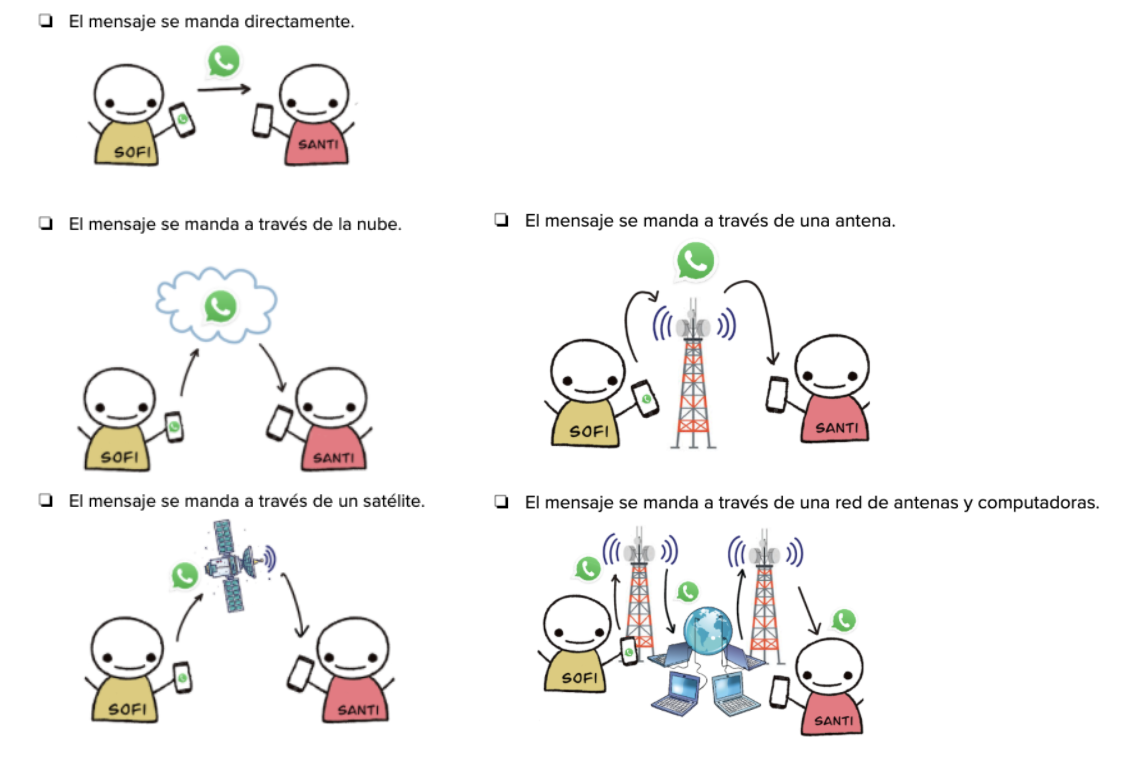
\includegraphics[width=0.90\textwidth]{images/1.png}
    \caption{Posibles opciones de respuesta para la pregunta acerca de la conectividad móvil.}
    \label{fig:cuest1}
\end{figure}

\subsection{Gratuidad de las aplicaciones en Internet}

Por último, intentamos conocer qué piensan acerca de la gratuidad de las aplicaciones en Internet: ¿por qué pueden acceder a las aplicaciones que más utilizan sin pagar? ¿De qué manera ganan dinero Facebook, YouTube, TikTok e Instagram?

La pregunta que les proponemos en la encuesta es: \textit{Muchas de las aplicaciones que conocemos se pueden usar gratuitamente, como por ejemplo Facebook, YouTube, Instagram o TikTok. ¿Por qué creés que permiten su uso sin tener que pagar?}

\section{Primera iteración: encontrando la manera de preguntar}

Al encarar la construcción del cuestionario, nuestro objetivo principal fue encontrar la manera más clara de preguntarles sobre aquello que queremos investigar.   

Al diseñar un cuestionario cerrado, los y las participantes deberán responder a solas, por lo que es muy importante que las preguntas puedan ser interpretadas y entendidas de la manera menos ambigua posible, ya que no habrá intervención nuestra al momento de realizar la actividad.

Con este fin, evaluamos que en algunos casos era necesario elaborar un “camino de preguntas”, es decir, una sucesión de preguntas que los llevara a entender la pregunta que queríamos hacer finalmente o bien, que les permitiera entrar en contexto respecto del tema para entender qué era lo que queríamos preguntarles.

\begin{figure}[h]
    \centering
    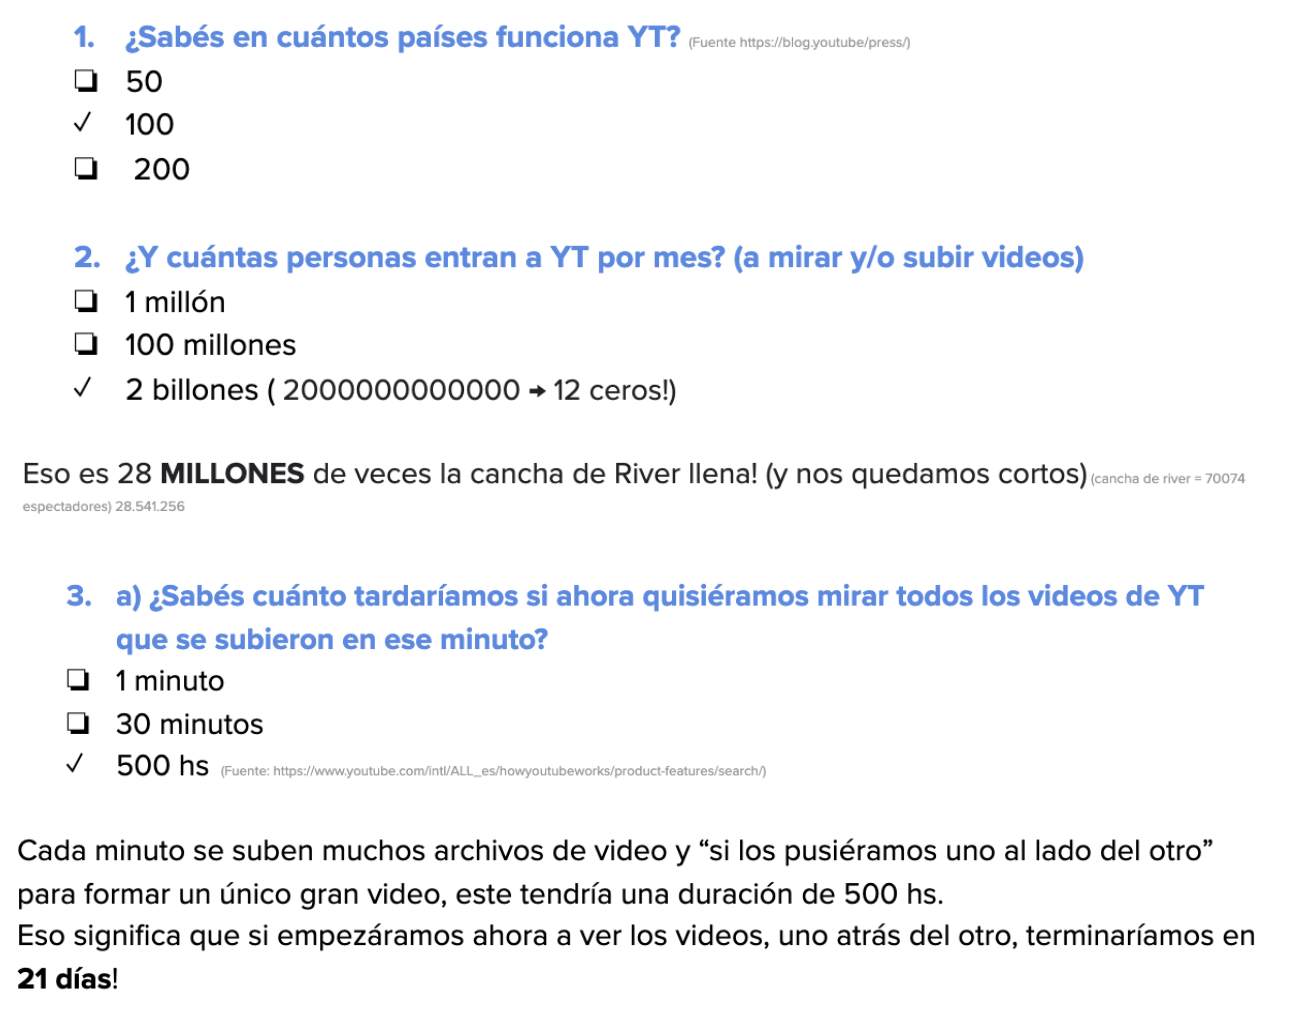
\includegraphics[width=0.75\textwidth]{images/2.png}
    \caption{Primera versión de la pregunta sobre almacenamiento de datos en YouTube, utilizando múltiples preguntas y únicamente texto.}
    \label{fig:cuest2}
\end{figure}

En la versión que se observa en la Fig \ref{fig:cuest2}, intentábamos dar a los niños y niñas una dimensión de la cantidad de datos que se almacenan en plataformas como YouTube. Sin embargo, hay que tener presente el no “guiarlos” en las preguntas, ya que no queremos “enseñarles” durante el cuestionario, o sesgar sus respuestas hacia una interpretación en particular, sino que puedan responder lo más libremente posible.

\section{Segunda iteración: refinando las preguntas}

Realizamos distintas rondas de mejoras y cambios en la encuesta hasta llegar a la versión final. En cada una de estas iteraciones, trabajamos en encontrar cuál era el equilibrio entre dar contexto a una pregunta (realizando múltiples preguntas sobre el mismo tema) y guiar demasiado a una respuesta determinada o limitar la posibilidad de responder independientemente.  

Así por ejemplo, iteramos en la pregunta anterior repensando cómo abordar la noción de los datos almacenados en YouTube y agregando imágenes, como podemos observar en la Fig \ref{fig:cuest3}.

\begin{figure}[h]
    \centering
    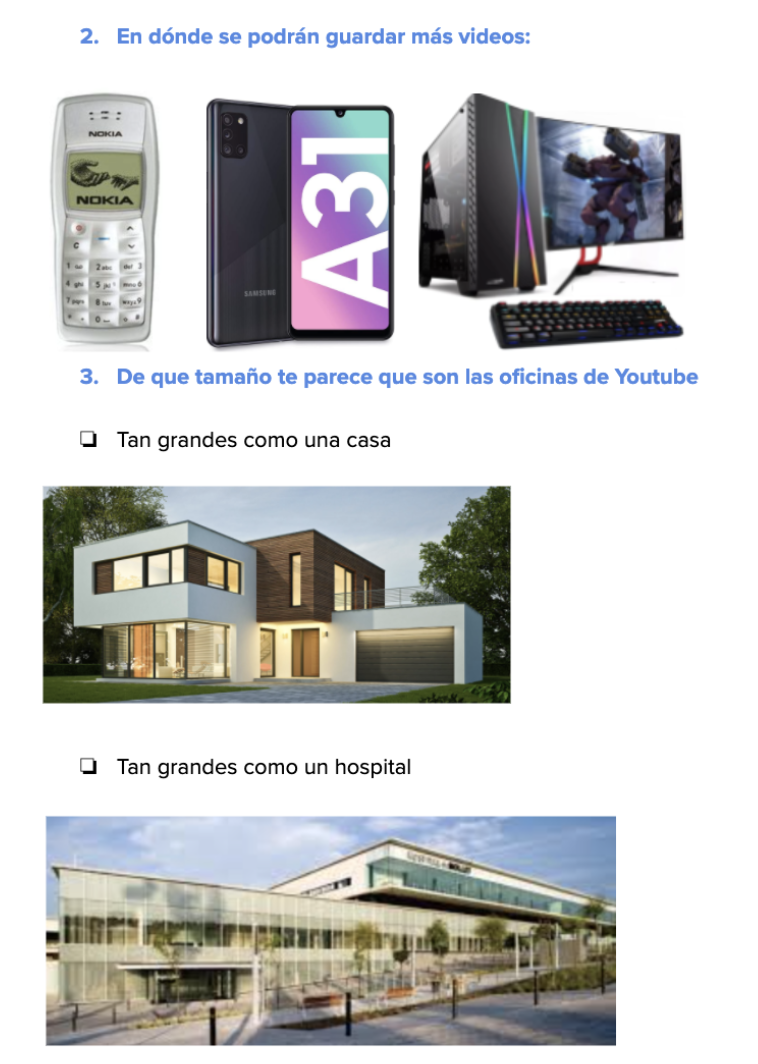
\includegraphics[width=0.5\textwidth]{images/3.png}
    \caption{Segunda versión, utilizando imágenes.}
    \label{fig:cuest3}
\end{figure}

\section{Tercera iteración: llegando a una versión más cerrada}

Ya en una tercera iteración del cuestionario, decidimos encarar la pregunta relacionada al almacenamiento de datos en YouTube de una manera más directa, pero apoyándonos en ilustraciones que nos permitieran ejemplificar las respuestas, como podemos ver en la Fig \ref{fig:cuest4}. Valiéndonos de esta ayuda visual, intentamos que el tema sea más accesible.

\begin{figure}[h]
    \centering
    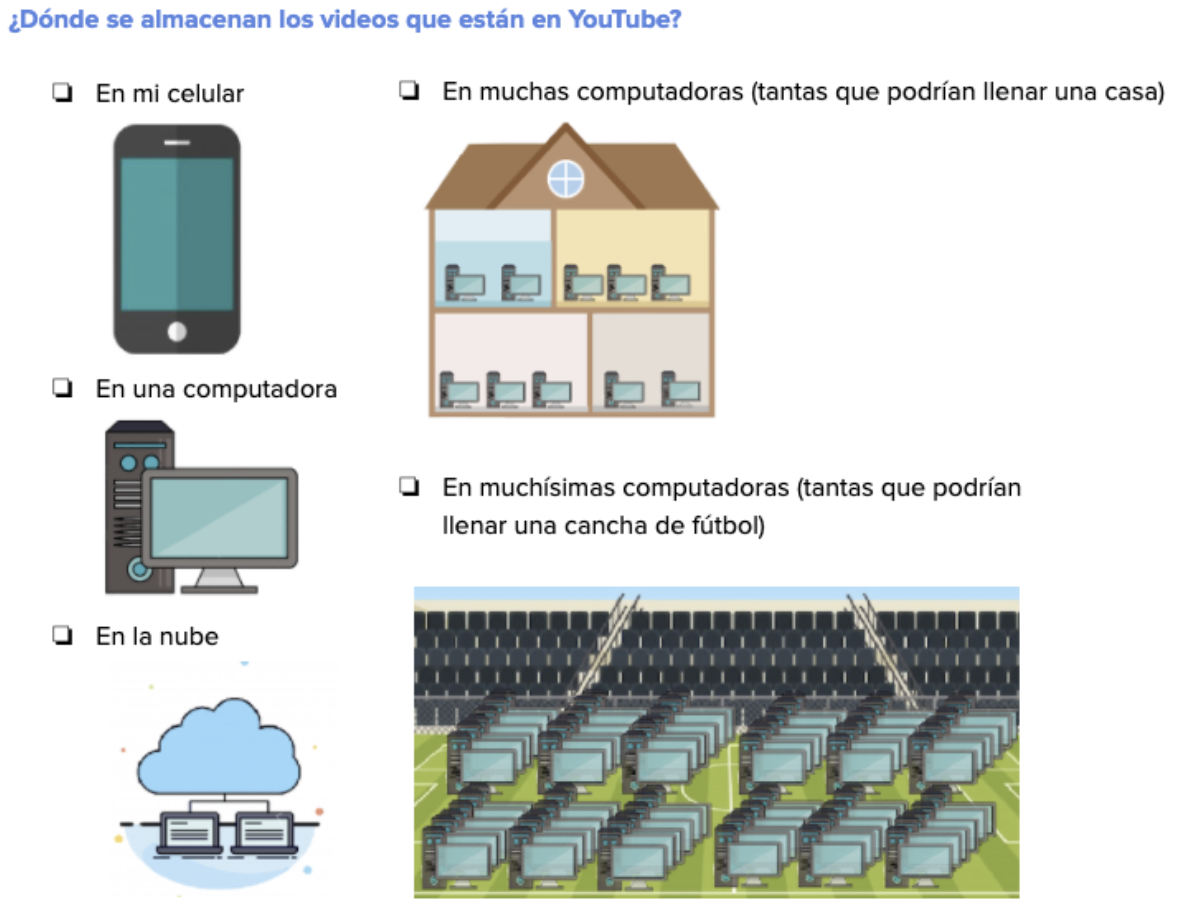
\includegraphics[width=0.8\textwidth]{images/4.png} 
    \caption{Tercera versión, utilizando ilustraciones.}
    \label{fig:cuest4}
\end{figure}

\newpage

\section{Anonimato y datos poblacionales}

Si bien la participación de los chicos y chicas en el cuestionario fue de carácter anónimo, es decir, no quedaron registrados sus datos personales de ninguna manera, agregamos una sección de preguntas poblacionales, destinadas a clasificar posteriormente la información en función de algunas variables demográficas, tales como edad y género. También les solicitamos información relativa al uso de computadoras y celulares (dónde y cuándo los utilizan, cómo aprendieron a hacerlo y cuál es el uso mayoritario que le dan a ambos dispositivos).     

Por último, recolectamos datos relacionados al contexto social de la escuela a la que asisten y a la carga académica de los alumnos en materias relacionadas a la Computación, Informática o Ciencias de la Computación para, de esta manera, tener un panorama más amplio del contexto de los niños y niñas que participan de nuestro estudio.

\section{Pruebas piloto}

Como paso previo a difundir la encuesta decidimos realizar una serie de pruebas piloto. Estas tuvieron como objetivo comprobar si las preguntas que realizamos son bien comprendidas, si las imágenes que las acompañan ayudan a clarificarlas y no generan confusiones, y si los temas son adecuados. Además, les pedimos a los participantes de estas pruebas que nos dieran su opinión respecto del cuestionario: ¿Les pareció fácil? ¿Difícil? ¿Cambiarían algo? ¿Es necesario agregar alguna opción en alguna pregunta?

Realizamos las pruebas pilotos en dos etapas. En la primera etapa entrevistamos a tres niñas y niños de alrededor de 10 años. Comenzamos teniendo una entrevista con el adulto responsable, en la que le explicamos acerca de la actividad, cómo sería realizada y del carácter anónimo de la misma. Además, le pedimos que no ofreciera su ayuda ni interviniera en ningún momento, de manera de no condicionar sus respuestas. A continuación, tuvimos una breve presentación con los chicos y chicas, en la que les explicamos el objetivo del cuestionario y les pedimos que completaran la encuesta.

Cabe destacar que, como realizamos las entrevistas en un contexto remoto, les pedimos a los tres participantes que nos compartieran su pantalla para poder ver cómo completaban la encuesta en tiempo real y, de esta manera, tratar de imitar lo más posible la presencialidad.  Esto nos proveyó de una información muy rica, ya que fuimos capaces de ver sus expresiones al leer las preguntas e identificar qué partes les eran confusas o les presentaban mayor dificultad. 

Como resultado de la primera vuelta de pruebas piloto, pudimos corroborar que las temáticas elegidas les eran conocidas y que las tecnologías indagadas eran utilizadas por ellos en su vida diaria.

También nos expresaron que en algunos casos habían tenido dificultad para entender lo que se les estaba preguntando, siendo lo más señalado la pregunta referida a la conectividad de los celulares.

A partir del \textit{feedback} recibido, decidimos reducir la cantidad de opciones que ofrecíamos como posibles respuestas, ya que nos pareció que el inconveniente radicaba en las diferencias sutiles que había entre ellas. 

\begin{figure}[h]
    \centering
    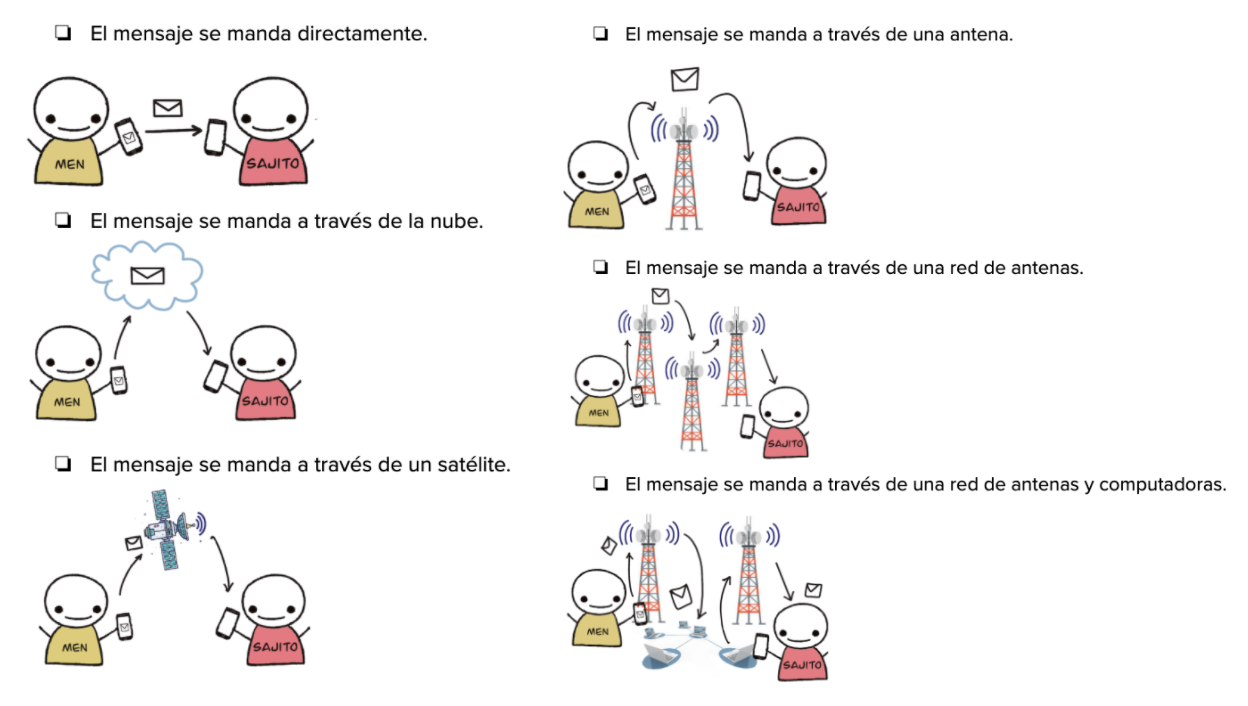
\includegraphics[width=0.8\textwidth]{images/5.png} 
    \caption{Versión inicial.}
    \label{fig:cuest5}
\end{figure}


\begin{figure}[h]
    \centering
    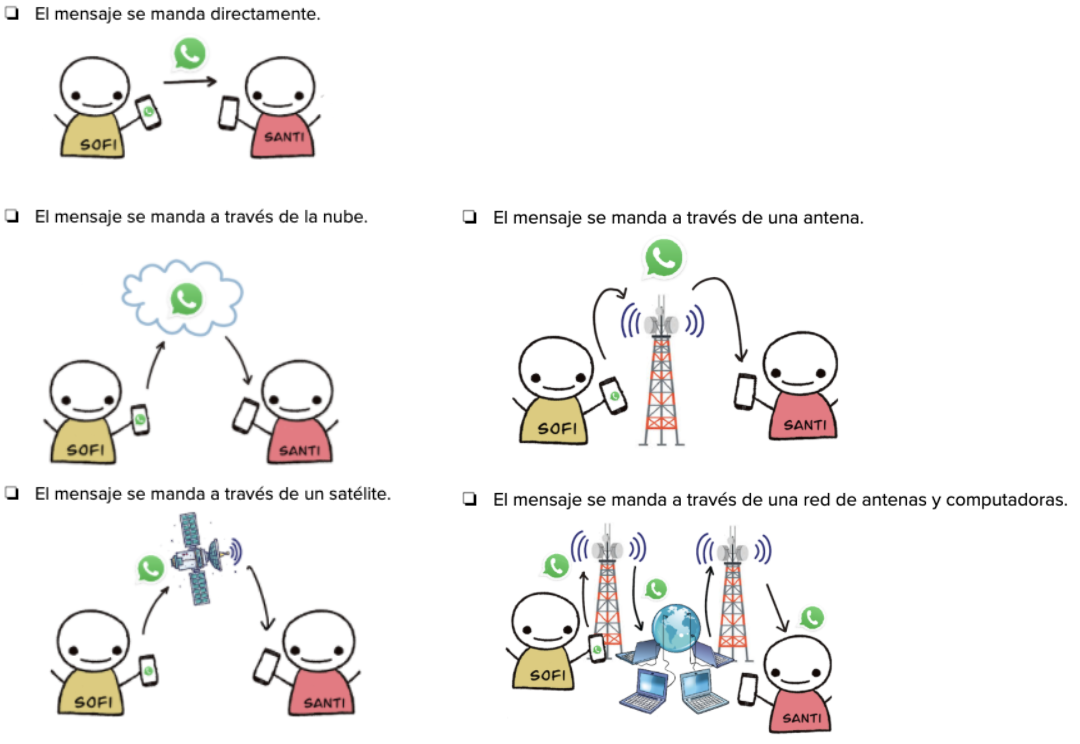
\includegraphics[width=0.7\textwidth]{images/6.png} 
    \caption{Versión final.}
    \label{fig:cuest6}
\end{figure}


En el caso de la Fig \ref{fig:cuest5} podemos ver la primera versión de la pregunta sobre conectividad donde había más opciones para elegir: una antena, múltiples antenas o antenas y computadoras. Pasamos finalmente a una versión más simplificada, como se observa en la Fig \ref{fig:cuest6}, en la que la cantidad de opciones alcanza para evaluar si los niños y niñas tiene una \textit{misconception} al respecto.

Por otro lado, aprovechamos para clarificar además el tipo del mensaje al que se refiere la pregunta (en este caso, cambiando el dibujo genérico de un sobre por el logo de WhatsApp), ya que habíamos notado que no había quedado del todo claro al tipo de mensaje al que la pregunta apuntaba, y eso había generado dudas en algunos casos. 

\newpage

Otra cuestión recurrente en las entrevistas de prueba fue que la pregunta relativa a la gratuidad de las aplicaciones en Internet no les había resultado fácil ya que tenía mucho texto para leer. Para tratar de hacerla un poco más amena, pensamos en agregar ilustraciones que acompañen las opciones. Inicialmente evaluamos utilizar ilustraciones similares a las usadas anteriormente como se observa en la Fig \ref{fig:cuest7}. 

\begin{figure}[h]
    \centering
    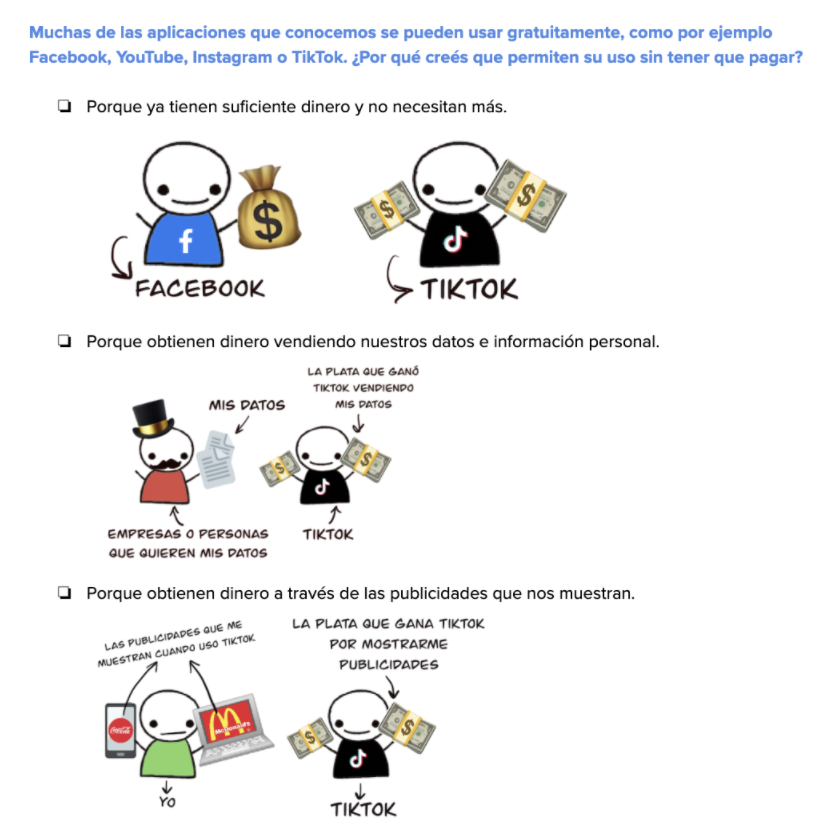
\includegraphics[width=0.7\textwidth]{images/7.png} 
    \caption{Versión inicial.}
    \label{fig:cuest7}
\end{figure}

Si bien esta opción nos parecía más simpática, decidimos ir por otro camino, ya que era posible que los dibujos sesgaran o influenciaran la respuesta. Por este motivo terminamos utilizando imágenes de textos acompañados por emojis, como podemos ver en la Fig \ref{fig:cuest8}, que facilitan la interpretación de las opciones pero que tienen menor impacto visual.

\begin{figure}[h]
    \centering
    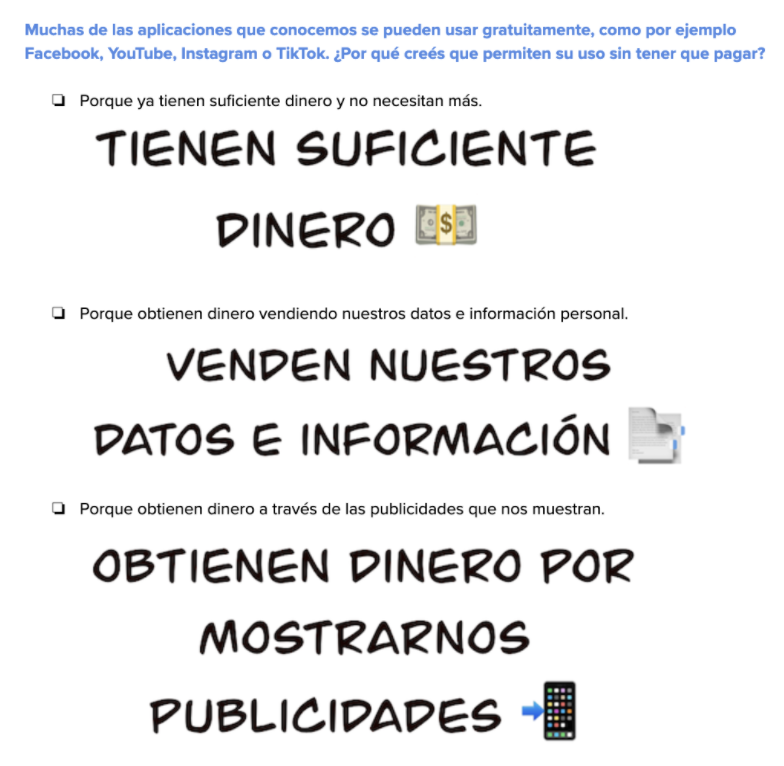
\includegraphics[width=0.6\textwidth]{images/8.png} 
    \caption{Versión final.}
    \label{fig:cuest8}
\end{figure}

Por último, agregamos a todas las preguntas la opción “No sé” ya que nos dimos cuenta en las pruebas piloto que a veces los chicos y chicas respondían cualquiera de las opciones cuando no entendían la pregunta o no conocían sobre el tema. De esta manera, les permitimos tener otra posibilidad de respuesta ante estos casos.

Tras terminar estos cambios, realizamos una segunda etapa de entrevistas y pudimos corroborar que las dificultades planteadas anteriormente se atenuaron, con lo que dimos por concluida la etapa del diseño del cuestionario. La versión final del mismo se encuentra disponible en el \autoref{chap:anexo}. 

\chapter{Análisis de resultados}
\section{Descripción del grupo}

\subsection{Grupo encuestado}

En Abril de 2021 lanzamos una convocatoria en la que le pedimos a docentes de escuelas argentinas que estuvieran dando clases a alumnos de alrededor de 10 años que nos contactaran para colaborar en la actividad.

Logramos coordinar con una docente de una escuela pública de Rosario, Santa Fé para que participara junto con sus alumnos de 4to y 5to grado, siendo en total 144 niños y niñas.

Ese mismo mes y a lo largo de dos semanas, en la medida que la docente tenía clases con estos cursos, fue proponiéndoles que completen la encuesta y de esta forma fuimos recibiendo sus respuestas. 

Las respuestas recibidas en días posteriores no fueron tenidas en cuenta, ya que no teníamos certeza de que las respuestas reflejaran el conocimiento o las concepciones de los chicos (podría pasar que, al contestar por fuera del marco de la clase, no cumplieran la consigna de no buscar información en Internet o preguntar a otras personas).

Cabe destacar que, en el momento en el que se realizó la convocatoria, en Argentina se estaba transicionando de una vuelta a la presencialidad a el dictado de clases de manera online, por lo que muchas escuelas se encontraban organizándose frente a este cambio y no tenían disponibilidad para realizar la actividad con sus alumnos. Por este motivo, no nos fue posible conseguir otras escuelas que pudieran participar.

\subsection{Análisis Poblacional}

A continuación se describe el grupo encuestado según distintas variables poblacionales. 

\begin{figure}[h]
    \centering
    \begin{minipage}{0.50\textwidth}
        \centering
        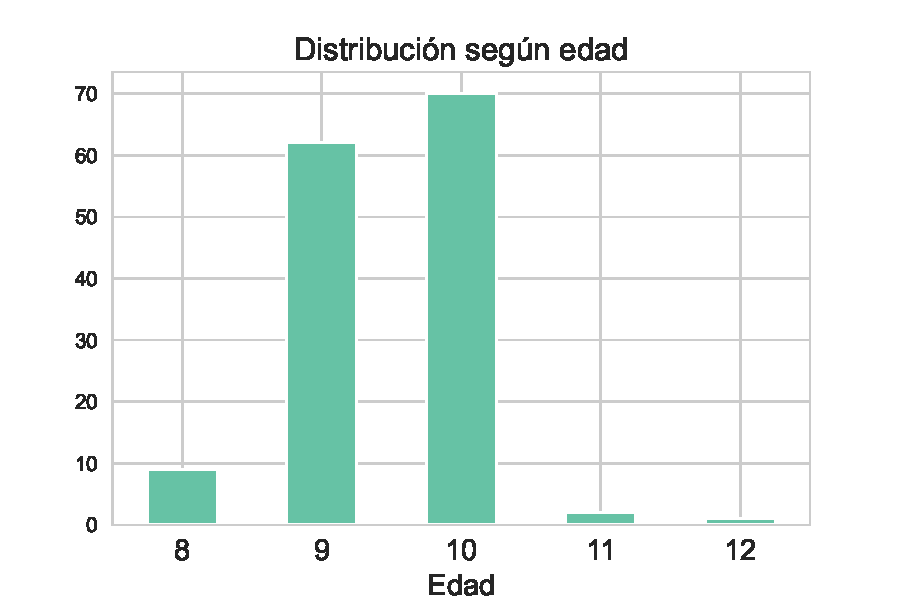
\includegraphics[width=0.9\textwidth]{images_analisis/1.pdf} 
        \caption{Participantes distribuidos por edad.}
        \label{fig:analisis1}
    \end{minipage}\hfill
    \begin{minipage}{0.50\textwidth}
        \centering
        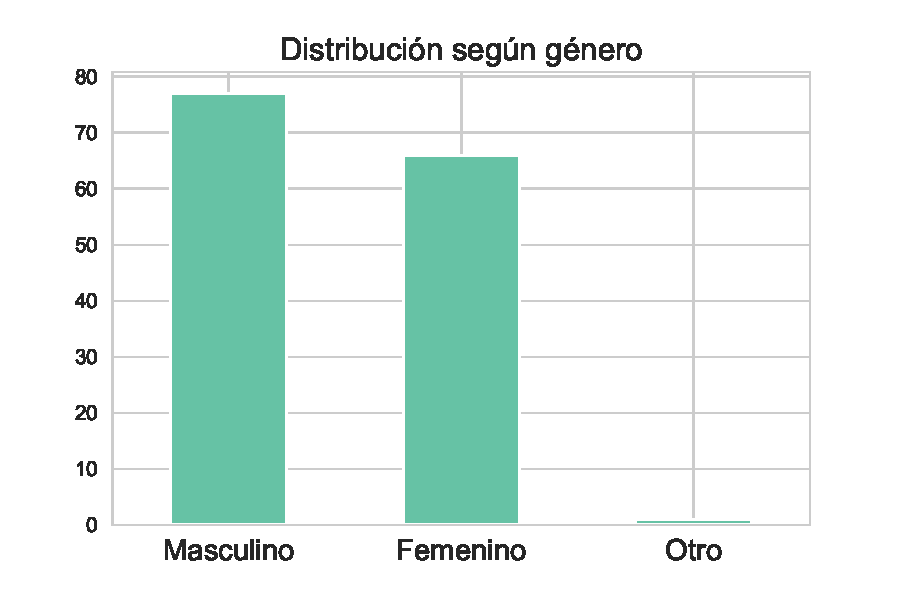
\includegraphics[width=0.9\textwidth]{images_analisis/2.pdf} 
        \caption{Participantes distribuidos por género}
        \label{fig:analisis2}
    \end{minipage}
\end{figure}

Podemos ver en la Fig. \ref{fig:analisis1} que se trata de un grupo bastante homogéneo en cuanto a la edad, en tanto es el objeto de nuestro estudio el grupo comprendido por niños y niñas de alrededor de diez años. En cuanto al género, observamos en la Fig. \ref{fig:analisis2} que tenemos también una distribución muy pareja.

Tras analizar la Fig. \ref{fig:analisis3} nos queda claro que la mayor parte de los participantes utilizan la computadora en su casa. Siendo que tanto este año como el anterior vivimos en un contexto de pandemia, este resultado no resulta sorprendente.

Podemos destacar que la mayoría parecieran contar con una computadora en sus hogares, siendo tan solo uno de ellos quien respondió que no poseía una.

También les preguntamos para qué utilizan más comúnmente la computadora. Les dimos la posibilidad de marcar más de una opción dentro de una serie de respuestas y, al mismo tiempo, dejamos un espacio disponible para poder completar con otras actividades que no estuvieran dentro de las que les habíamos propuesto.

\begin{figure}[h]
    \centering
    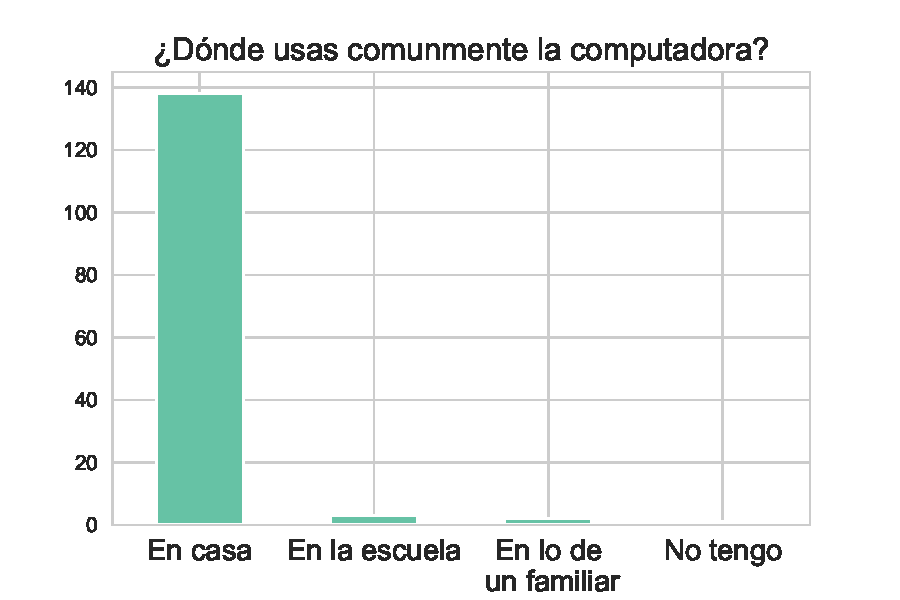
\includegraphics[width=0.5\textwidth]{images_analisis/3.pdf}
    \caption{Lugar en el que los participantes más usan la computadora.}
    \label{fig:analisis3}
\end{figure}

Es posible observar en la Fig. \ref{fig:analisis4} que la mayor parte de los encuestados utiliza la computadora para jugar juegos, siendo las siguientes actividades más usuales mirar videos en YouTube, realizar videollamadas utilizando Skype, Meet o Zoom, y realizar actividades escolares. Nuevamente, esto tiene sentido ya que durante todo el 2020 en Argentina hubo clases de manera virtual.

\begin{figure}[h]
    \centering
    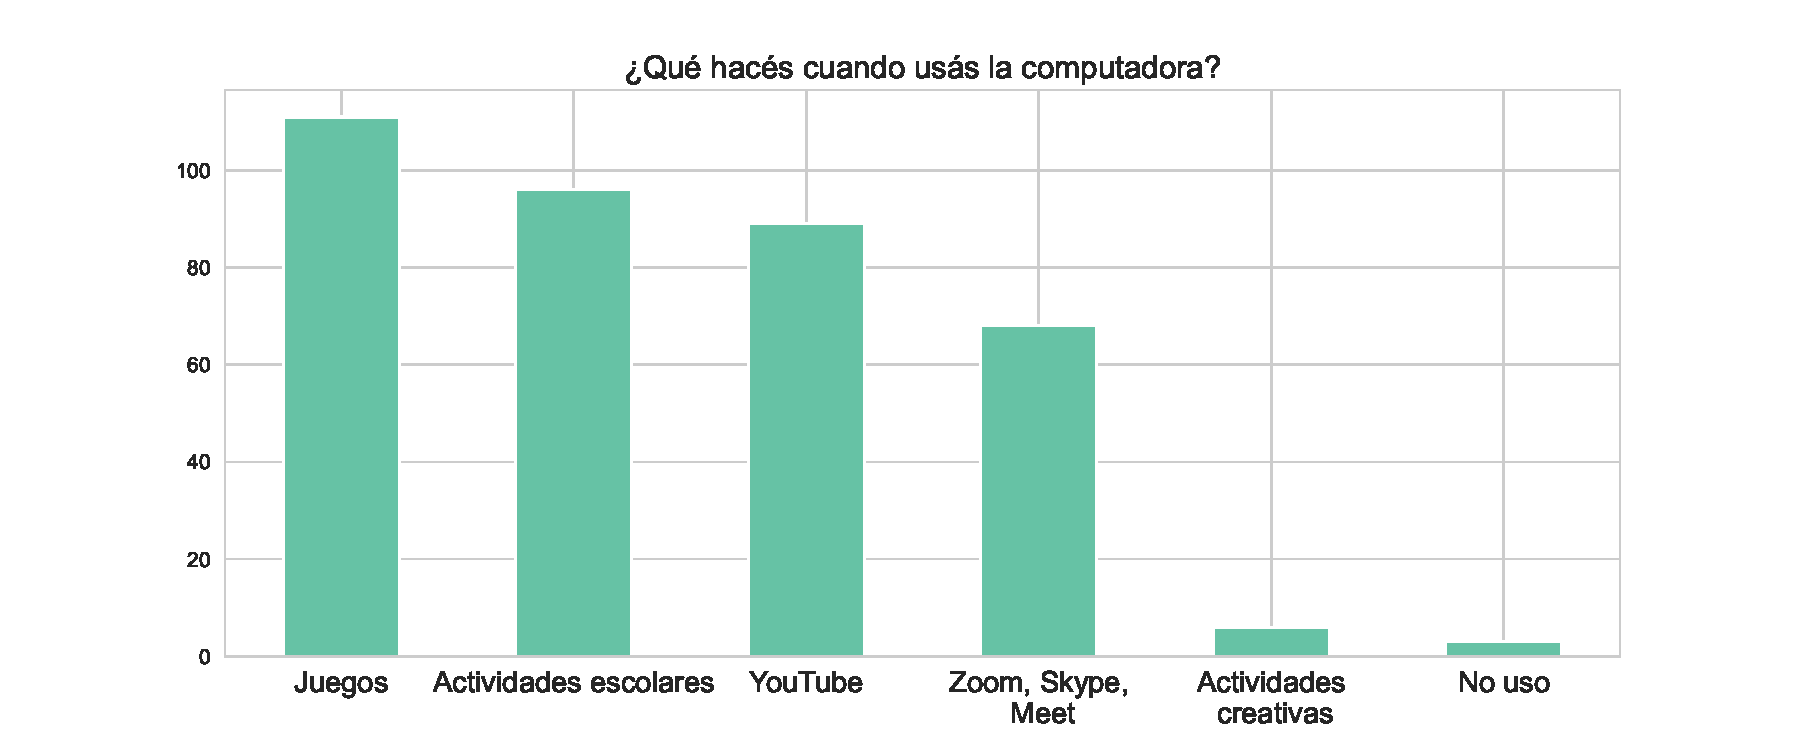
\includegraphics[width=1\textwidth]{images_analisis/4.pdf}
    \caption{Actividades más comunes al utilizar la computadora.}
    \label{fig:analisis4}
\end{figure}

\begin{figure}[h]
    \centering
    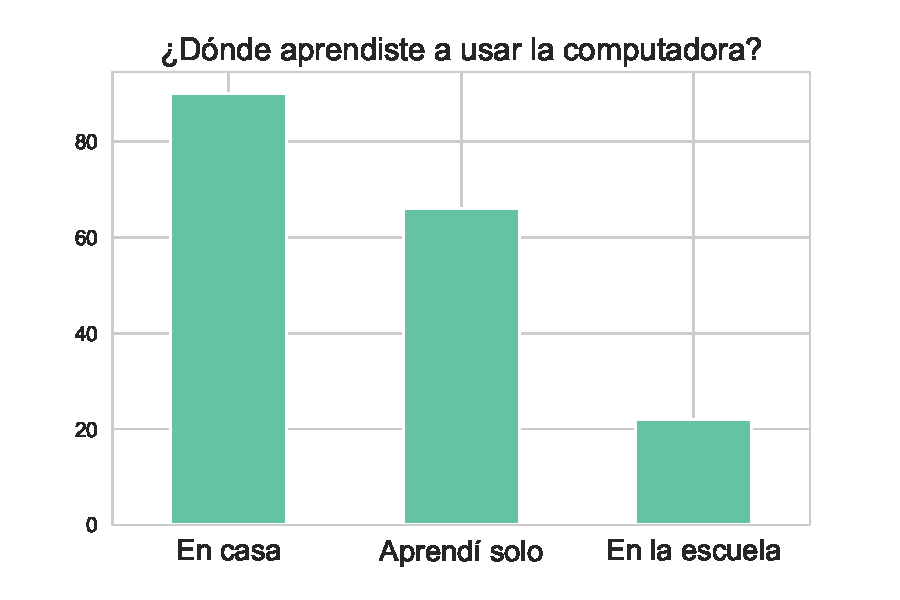
\includegraphics[width=0.50\textwidth]{images_analisis/5.pdf}
    \caption{Lugar o forma en la que aprendieron a utilizar la computadora.}
    \label{fig:analisis5}
\end{figure}

En cuanto a la forma en la que aprendieron a usar la computadora, se puede ver en la Fig. \ref{fig:analisis5} que las opciones más elegidas son ``\textit{Me enseñaron en mi casa (mis padres, hermanos u otro familiar)}'' y ``\textit{Aprendí solo}''.

Podemos ver que la tendencia está claramente más orientada a la formación recibida en el hogar, tanto por la enseñanza directa por parte de la familia o bien tal vez por la observación o la experiencia indirecta, al ver a otros miembros de la familia.

Esta hipótesis es respaldada por otros estudios anteriores, como por ejemplo el de Mertala \cite{mertala}, que explica que el conocimiento de los chicos sobre las distintas tecnologías se basa en el contacto que tuvieron con estas a través de sus padres, hermanos u otras figuras del entorno familiar o escolar.

De esta forma, esta percepción de haber ``aprendido solos'' podría tener raíz en este contacto indirecto.

Al indagar en la forma en que los chicos y chicas utilizan los celulares nos encontramos con que la gran mayoría cuenta con un dispositivo propio, como se puede observar en la Fig. \ref{fig:analisis6}.

\begin{figure}[h]
    \centering
    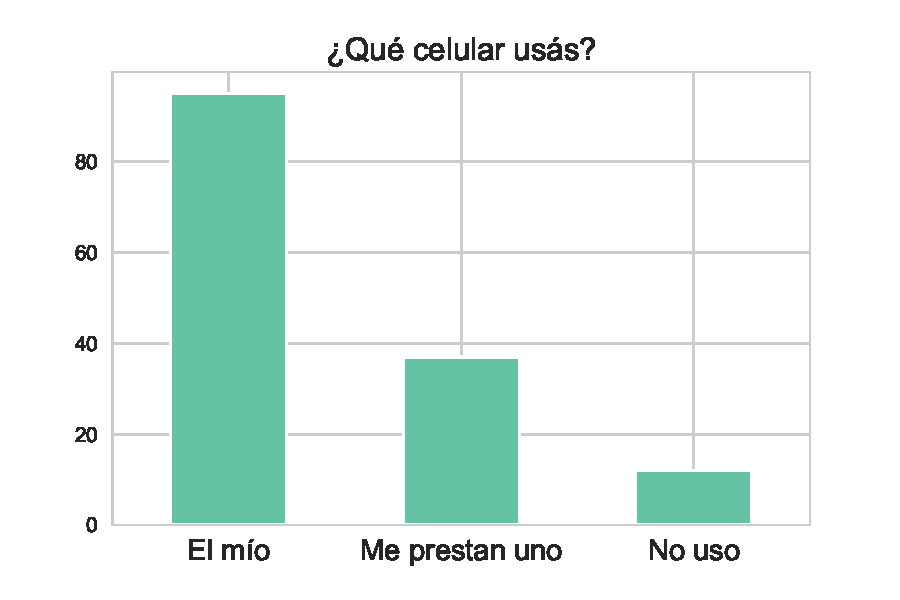
\includegraphics[width=0.6\textwidth]{images_analisis/6.pdf}
    \caption{Tipo de celular que utilizan (propio o prestado).}
    \label{fig:analisis6}
\end{figure}

En la Fig. \ref{fig:analisis7} vemos que la actividad más realizada es nuevamente jugar juegos, pero se suma con mucha importancia también el chat (utilizando aplicaciones de mensajería tales como Whatsapp, Telegram, etc.) y mirar videos en YouTube.

\begin{figure}[h]
    \centering
    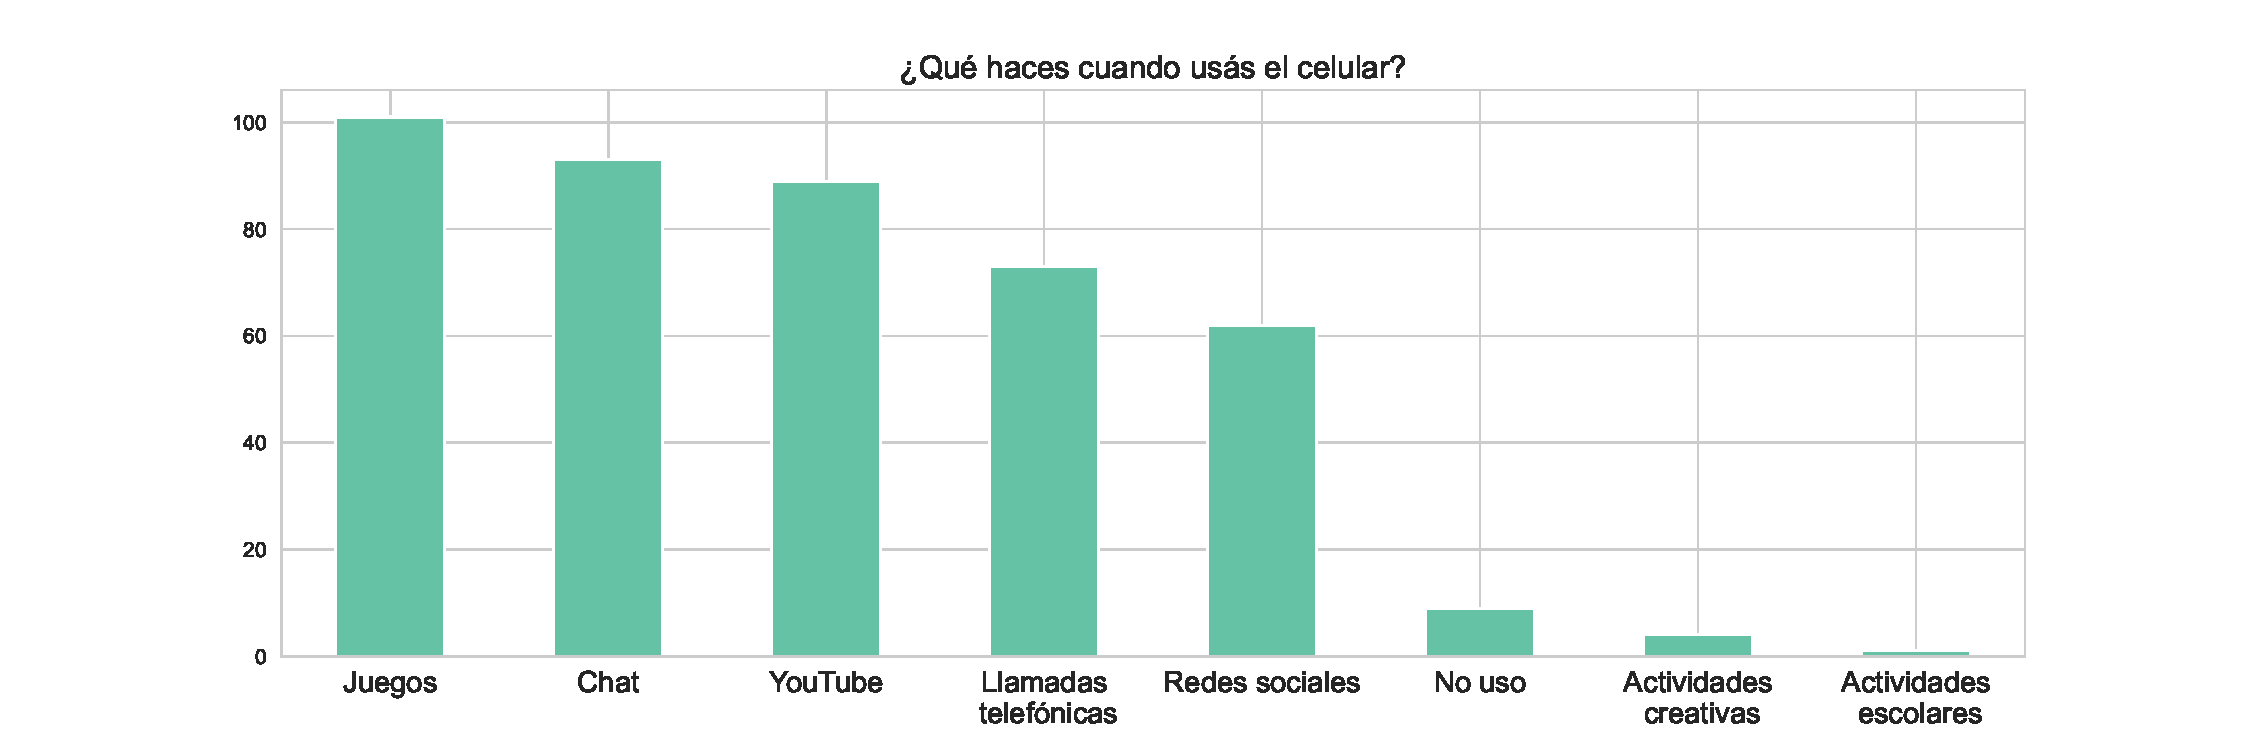
\includegraphics[width=1\textwidth]{images_analisis/7.pdf}
    \caption{Actividades más comunes al utilizar el celular.}
    \label{fig:analisis7}
\end{figure}


Es llamativo que haya aparecido ``\textit{Llamadas telefónicas}'' como una actividad de una importancia considerable, aunque cabe preguntarse si habría que haber pedido que especifiquen si se referían a videollamadas utilizando las aplicaciones anteriormente mencionadas y, en tal caso, la actividad ``\textit{Chat}'' cobraría aún más relevancia.

Dentro de ``\textit{Redes Sociales}'' se incluyen ejemplos como TikTok, Instagram y Facebook, aunque no les pedimos que especifiquen ninguna en particular. Sin embargo, sabemos por la consulta realizada previamente a la confección de la encuesta que realizamos a los referentes pedagógicos de la Fundación Sadosky que trabajan para el Plan Ceibal, que la red social elegida por sobre las otras es en estos momentos TikTok.

Por último, cabe destacar que ``\textit{Actividades creativas}'' no fue una opción propuesta por nosotros en el cuestionario (tanto en esta pregunta como en la relacionada a las actividades realizadas con la computadora), sino que fue agregada por los chicos y chicas al momento de completar la encuesta. Dentro de este grupo, agrupamos respuestas que se referían a la edición de videos y fotos (tal vez para compartir en aplicaciones tales como TikTok o Instagram), escuchar música y escribir historias.

\section{Análisis exploratorio de \textit{misconceptions}}

\subsection{¿Dónde se almacenan los videos de YouTube?}

El primer tema a analizar es el almacenamiento de grandes volúmenes de datos en YouTube. Para esto le preguntamos a los chicos ``\textit{¿Dónde se almacenan los videos que están en YouTube?}'' y les dimos como opciones de respuesta:
\begin{itemize}
    \item En mi celular.
    \item En la nube.
    \item En una computadora.
    \item En muchas computadoras (tantas que podríamos llenar una casa).
    \item En muchísimas computadoras (tantas que podríamos llenar una cancha de fútbol)
    \item No sé.
\end{itemize}

Podemos ver en la Fig. \ref{fig:analisis8} un resultado inicial donde se muestra que la mayoría de ellos respondieron ``\textit{En la nube}''. 

\begin{figure}[h]
    \centering
    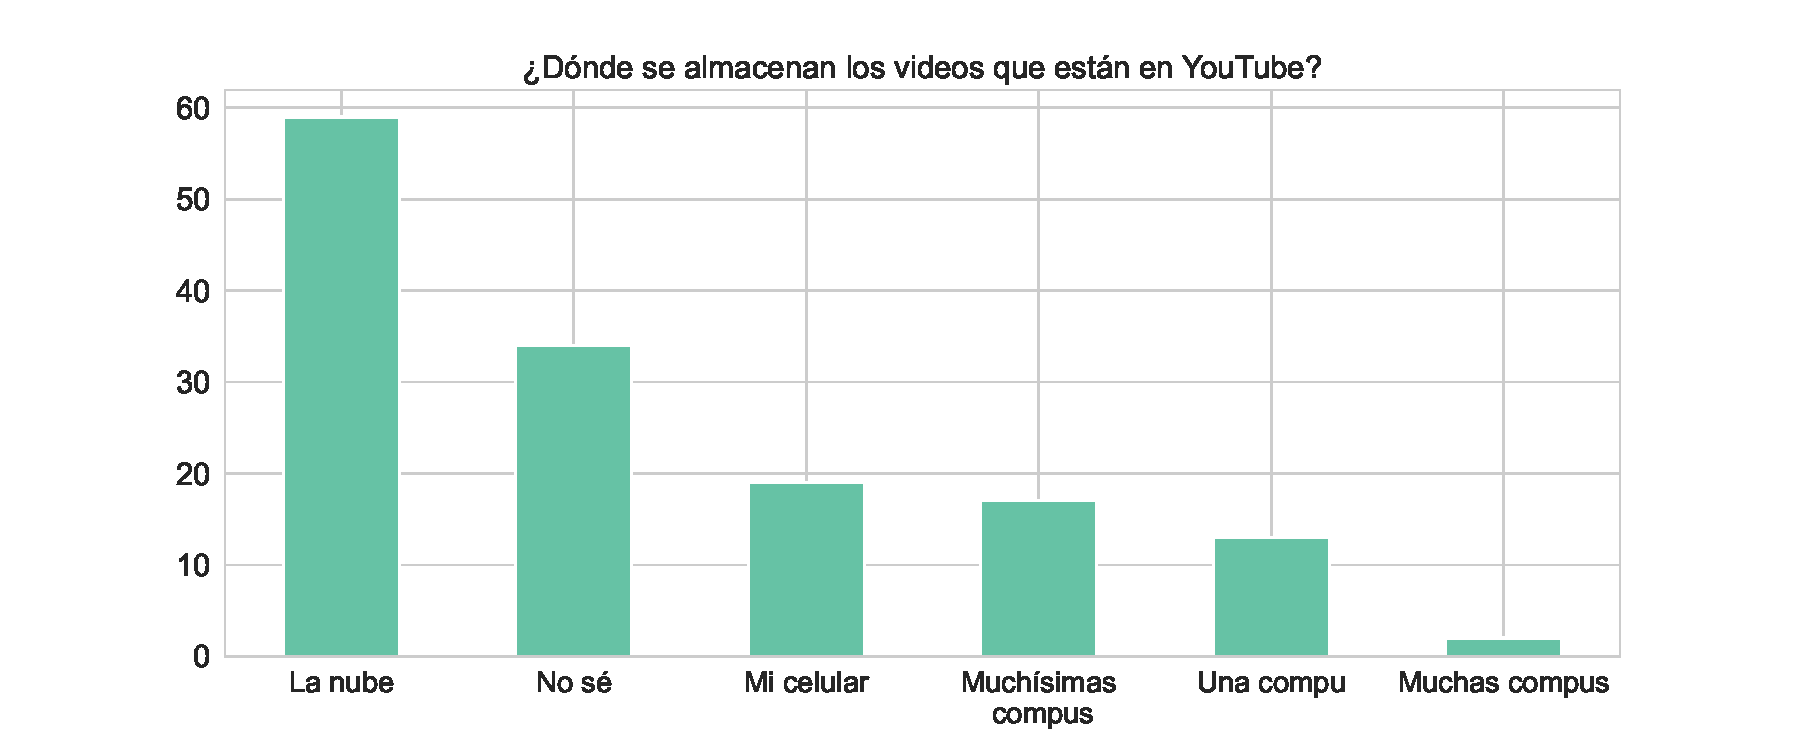
\includegraphics[width=1\textwidth]{images_analisis/8.pdf}
    \caption{Lugar en donde se almacenan los videos que están en YouTube.}
    \label{fig:analisis8}
\end{figure}

Esto es interesante porque el concepto de ``Nube'' es actualmente muy mencionado y por lo tanto está en el léxico de los chicos, a quienes seguramente Google les habrá ofrecido más de una vez ``\textit{más espacio de almacenamiento en la nube}'' (por nombrar un ejemplo). Sin embargo, cabe preguntarse si hay \textit{misconceptions} respecto de este tema puntual: ¿piensan a la nube como algo etéreo? ¿Qué cantidad de información ``entra'' en la nube? ¿Cómo funciona? Este es sin duda un tema interesante para seguir investigando a futuro.

En el siguiente lugar nos encontramos con la respuesta ``\textit{No sé}''. Esto deja en evidencia que este es un tema sobre el cual no se han preguntado mucho, incluso siendo que mirar videos en YouTube es la tercera actividad más elegida (tanto en la computadora como en el celular).

Luego, nos encontramos con una cantidad similar de respuestas con las opciones de ``\textit{En mi celular}'' y en ``\textit{Muchísimas computadoras (tantas que podríamos llenar una cancha de fútbol)}''. En el primer caso, está la \textit{misconception} de que el almacenamiento se da a nivel local, y más aún, que la cantidad de información a almacenar es tal que entraría en un celular. En el segundo caso, nos encontramos con la respuesta que propusimos como la más acertada, en la que queremos transmitir la idea de información distribuida a gran escala.

Por último, están quienes opinaron que la información se guarda en una sola computadora, con la idea de almacenamiento no distribuido, pero tal vez con más capacidad que un celular, y en ``\textit{En muchas computadoras (tantas que podríamos llenar una casa)}'', donde quisimos transmitir una noción de almacenamiento distribuido pero a una escala menor que en la opción de ``Muchísimas computadoras'' (tal vez incluso llevarlos a pensar en que las muchas computadoras podrían encontrarse en una oficina de YouTube o Google, pero todas en un mismo lugar físico).

En la Fig. \ref{fig:analisis9} podemos ver que la cantidad de alumnos con alguna \textit{misconception} en esta pregunta es casi el doble que la de alumnos sin \textit{misconception} (es decir, los niños y niñas que respondieron tanto la respuesta ``correcta'' como ``No sé'').

\begin{figure}[h]
    \centering
    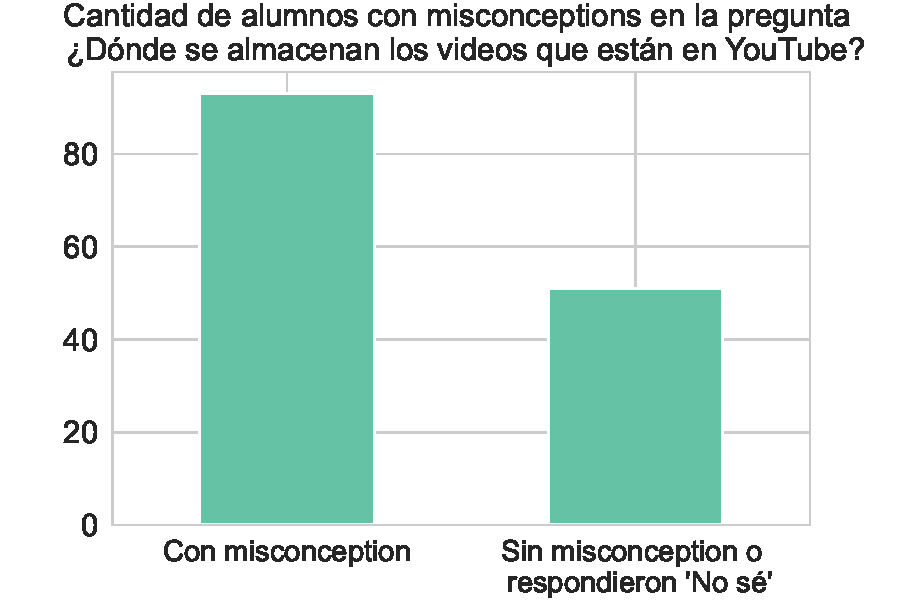
\includegraphics[width=0.6\textwidth]{images_analisis/9.pdf}
    \caption{Alumnos con \textit{misconception} vs sin \textit{misconception} en la pregunta sobre almacenamiento de videos en YouTube.}
    \label{fig:analisis9}
\end{figure}

\newpage

\subsection{¿De qué manera se comparte una foto por WhatsApp?}

La siguiente \textit{misconception} que queremos analizar es cómo es el mecanismo para compartir un archivo por WhatsApp.

En particular, vamos a profundizar en si, al compartir una imagen por este medio, se genera una copia que es la que se envía, o bien se comparte ``por referencia'', es decir, el archivo compartido no le queda en forma de copia a la otra persona, sino que está almacenado en algún servidor o dispositivo de almacenamiento y la persona a la que le fue compartido el archivo puede acceder a él de manera remota.  Más aún: queremos ver si está la noción de que, en este caso, hay un único archivo y que cuando, por ejemplo, éste se modifica, se modifica para todos los que lo ven, y cuando se elimina, se elimina para todos. 

En esta temática, nos pareció que preguntar directamente si una foto se comparte en WhatsApp por copia o referencia iba a generar confusión en los chicos, ya que estos conceptos tal vez no eran conocidos por ellos en estos términos.
De esta forma, pensamos que la mejor estrategia era elaborar un camino de preguntas que de cierto modo pudiera ponerlos en contexto dentro del tema sobre el cual nos interesaba indagar:

\begin{enumerate}
    \item ¿Quién tiene acceso a los archivos que tengo guardados en mi celular?
    \item Cuando comparto por WhatsApp un archivo que tenía guardado, ¿qué sucede? ¿Quién tiene el archivo enviado? ¿De qué manera accede la otra persona al mismo?
    \item ¿Qué pasa si ya no quiero compartir ese archivo? ¿Es posible? ¿Puedo perder la propiedad de un archivo que compartí por WhatsApp?
\end{enumerate}

\newpage

Para esto, la primera pregunta que les hicimos fue ``\textit{¿Quién tiene acceso a las fotos que tengo guardadas en mi celular?}''. En la Fig. \ref{fig:analisis11} podemos ver que la mayoría respondió que solo el dueño o la dueña del celular tiene acceso a las fotos guardadas en el dispositivo. De esta forma, como vemos en la Fig. \ref{fig:analisis10}, es mayor el número de alumnos sin \textit{misconception}.

\begin{figure}[h]
    \centering
    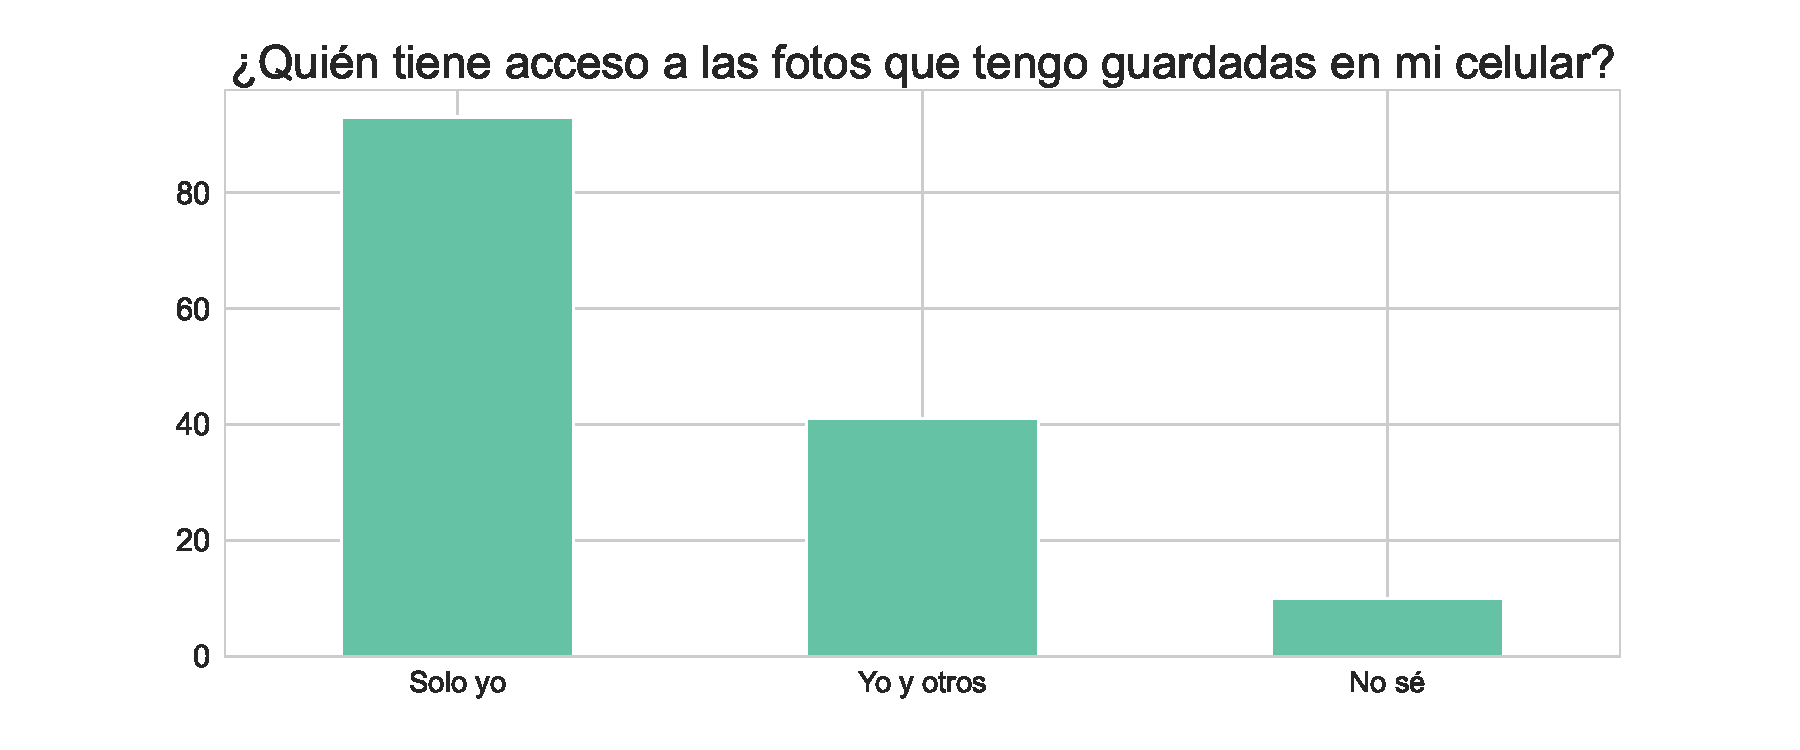
\includegraphics[width=0.8\textwidth]{images_analisis/11.pdf} 
    \caption{¿Quién tiene acceso a las fotos que tengo guardadas en mi celular?}
    \label{fig:analisis11}	
\end{figure}

\begin{figure}[h]
    \centering
    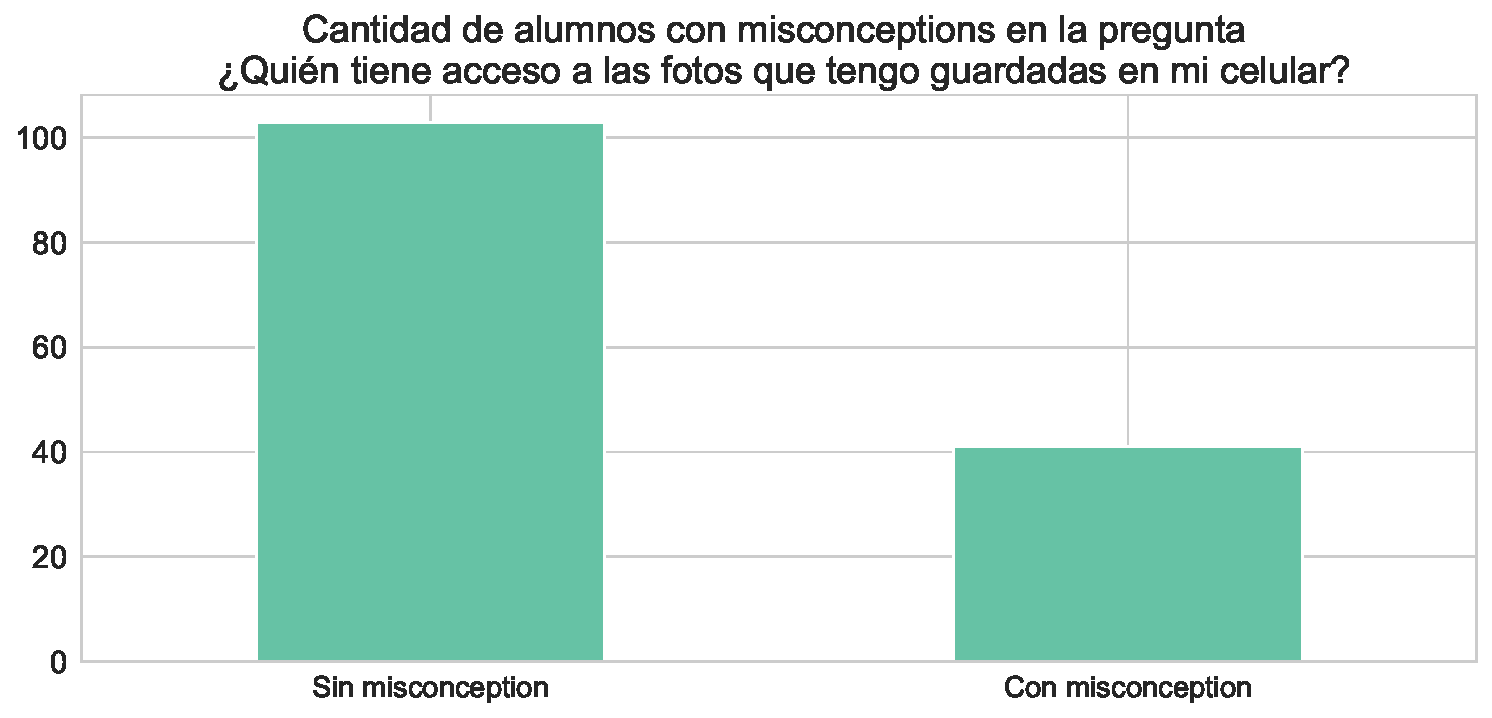
\includegraphics[width=0.8\textwidth]{images_analisis/10.pdf}
    \caption{Alumnos con \textit{misconception} vs sin \textit{misconception} en la pregunta sobre el acceso a fotos en un celular.}
    \label{fig:analisis10}
\end{figure}

Analizando ahora la siguiente pregunta, en la Fig. \ref{fig:analisis12} podemos ver que es bastante similar la cantidad de niños y niñas que opinan, por un lado, que cuando se envía una foto, lo que se manda es una copia y, por el otro, que esa foto ``existe en WhatsApp'' pero que la persona a la que se la enviaron no la tiene como copia en su celular. En esta última opción quisimos dar una idea de referencia.

\begin{figure}[h]
    \centering
    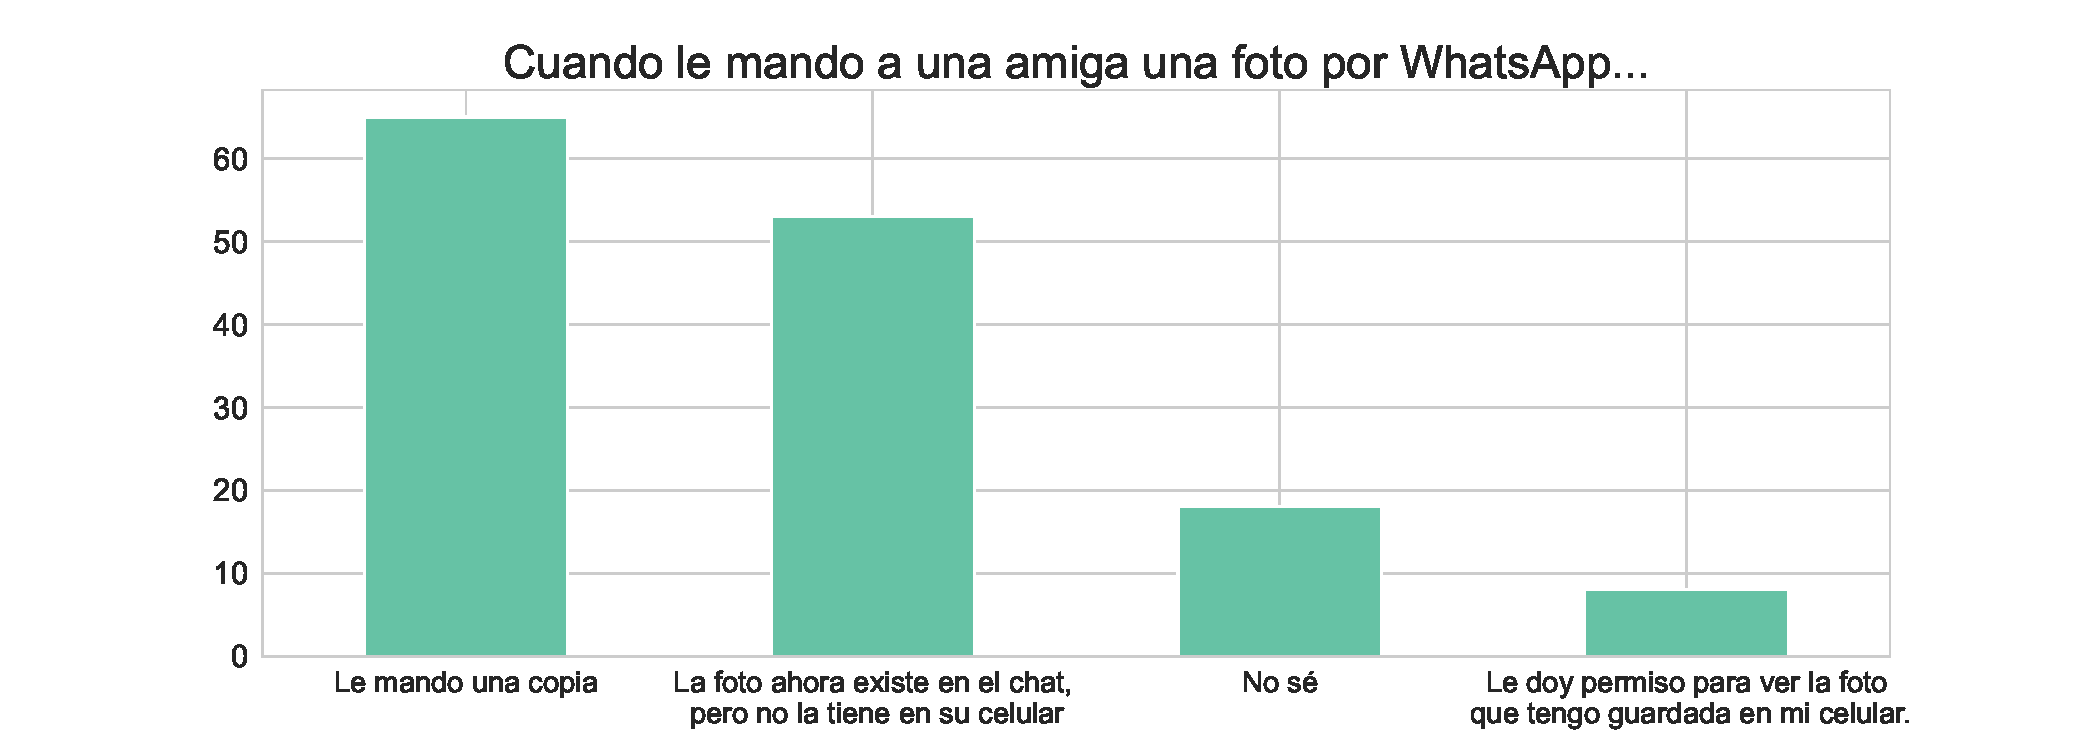
\includegraphics[width=0.9\textwidth]{images_analisis/12.pdf}
    \caption{ ¿Qué pasa cuando le envío a alguien por WhatsApp una foto que tengo en mi celular?}
    \label{fig:analisis12}
\end{figure}

De todas maneras, a pesar de que la respuesta más elegida es la ``correcta'', el número de encuestados y encuestadas con y sin \textit{misconceptions} es parecido. En la Fig. \ref{fig:analisis13} podemos observarlo.

\begin{figure}[h]
    \centering
    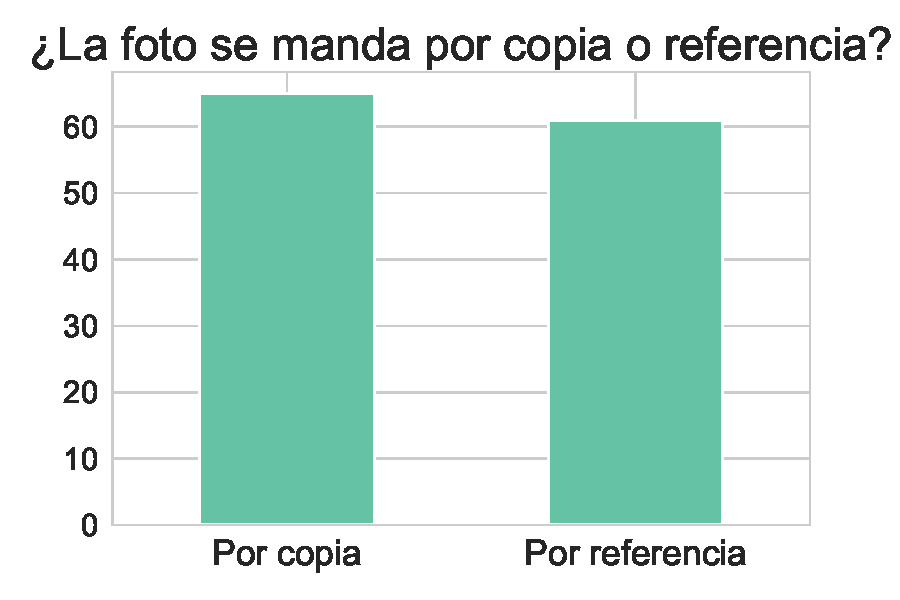
\includegraphics[width=0.4\textwidth]{images_analisis/13.pdf}
    \caption{Niños y niñas que muestran la idea de compartir archivos por copia o por referencia.}
    \label{fig:analisis13}
\end{figure}

\newpage

En la Fig. \ref{fig:analisis15} podemos ver que fueron bastantes los entrevistados que respondieron no saber acerca de este tema. 

\begin{figure}[h]
    \centering
    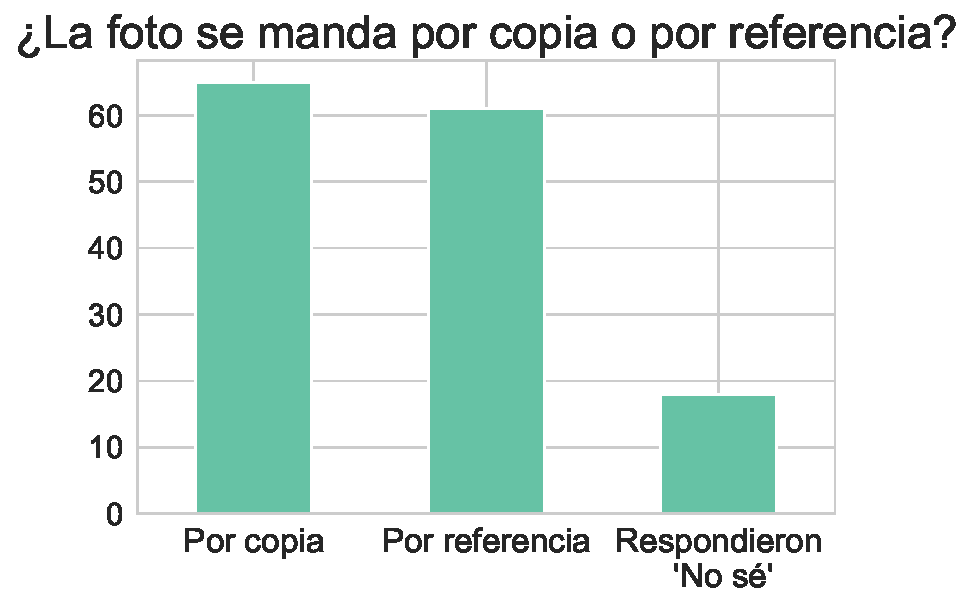
\includegraphics[width=0.4\textwidth]{images_analisis/15.pdf} 
    \caption{Alumnos que respondieron que la foto se manda por copia o referencia, diferenciando los que respondieron "No sé".}
    \label{fig:analisis15}
\end{figure}

\newpage

Sin embargo, considerando que responder “No sé” implica que no se tiene una concepción errónea (ya que justamente, se identifica una falta de conocimiento sobre un tema), podemos considerar a este grupo como dentro de los que no tienen \textit{misconceptions}. De esta forma, la distribución queda como vemos en la Fig. \ref{fig:analisis16}.

\begin{figure}[h]
    \centering
    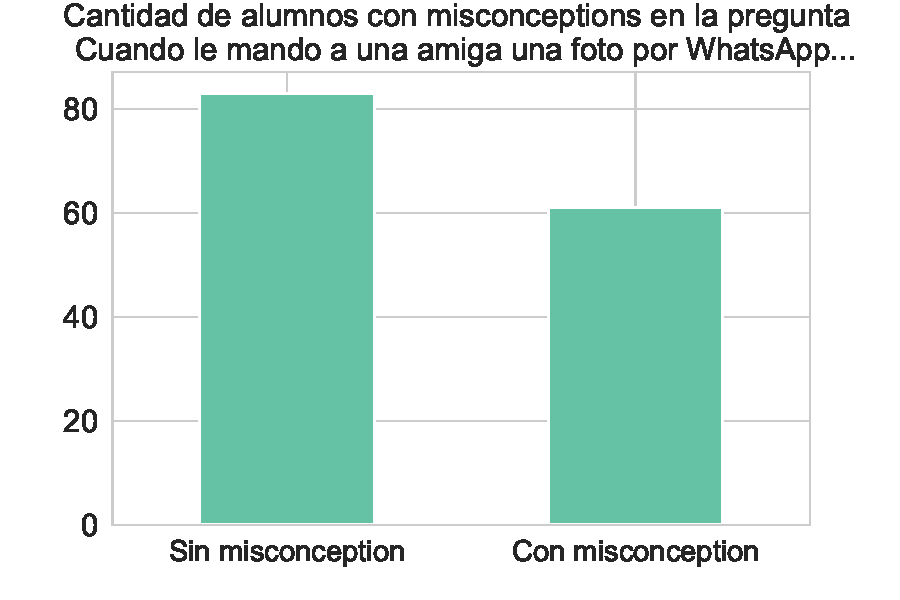
\includegraphics[width=0.5\textwidth]{images_analisis/16.pdf}
    \caption{Cantidad de alumnos con y sin \textit{misconceptions} en la pregunta sobre el envío de una foto por WhatsApp.}
    \label{fig:analisis16}
\end{figure}

Por último, como habíamos mencionado anteriormente en el punto 3, les preguntamos qué pueden hacer si quieren que la persona a la que le compartieron la foto no pueda acceder más a ella. En la Fig. \ref{fig:analisis17} podemos observar las respuestas de los chicos.

\begin{figure}[h]
    \centering
    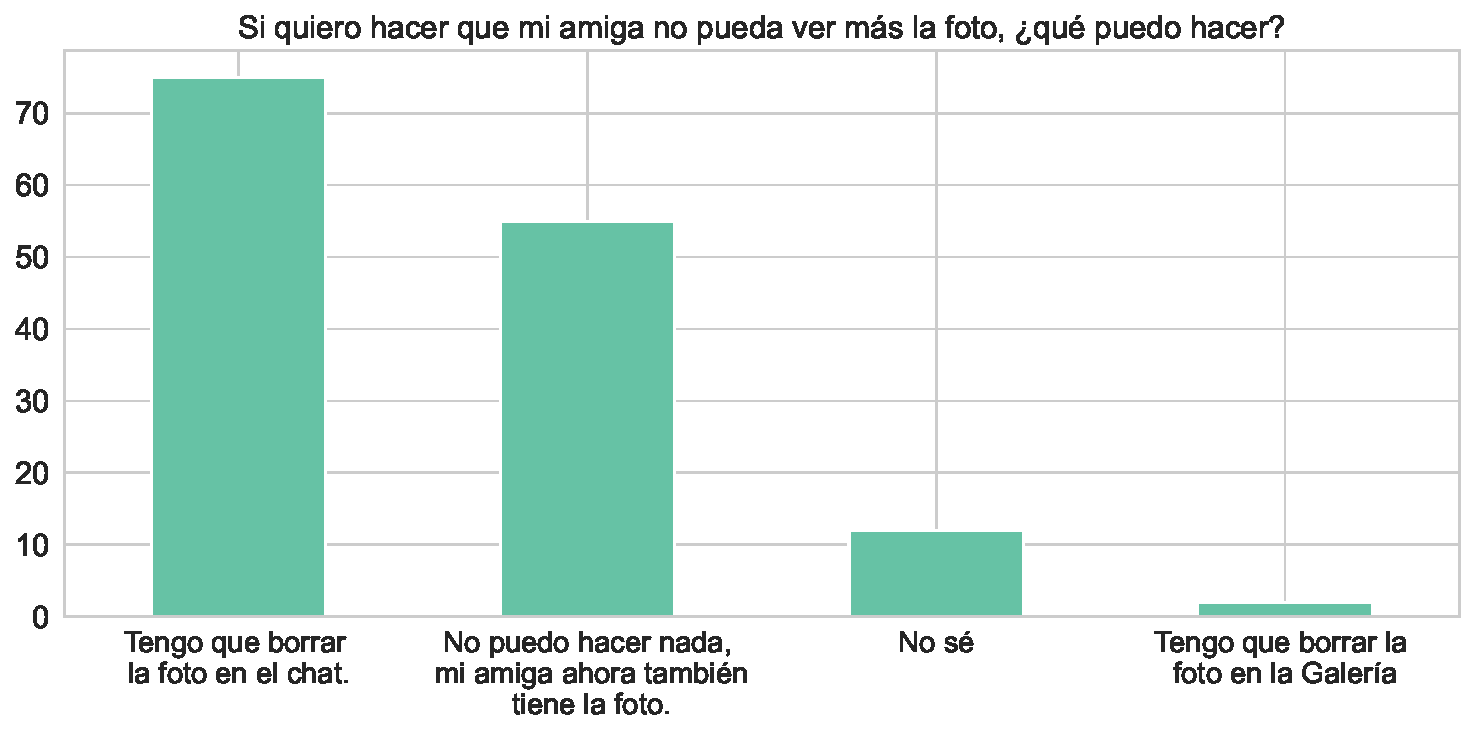
\includegraphics[width=0.95\textwidth]{images_analisis/17.pdf}
    \caption{¿Qué pasa si le compartí a alguien una foto y quiero quitarle el acceso a la misma?}
    \label{fig:analisis17}
\end{figure}

Con esta pregunta, intentamos relacionar los conceptos vistos anteriormente y dilucidar si la idea de copia y referencia estaba clara.

Al analizar los datos, nos encontramos con una sorpresa: si bien en las dos preguntas anteriores, la mayor parte de los niños y niñas encuestadas había contestado correctamente dando a conocer que los archivos se envían como una copia cuando se comparten por WhatsApp, en esta pregunta mostraron tener una \textit{misconception}, tal como se puede ver en la Fig. \ref{fig:analisis18}.

\begin{figure}[h]
    \centering
    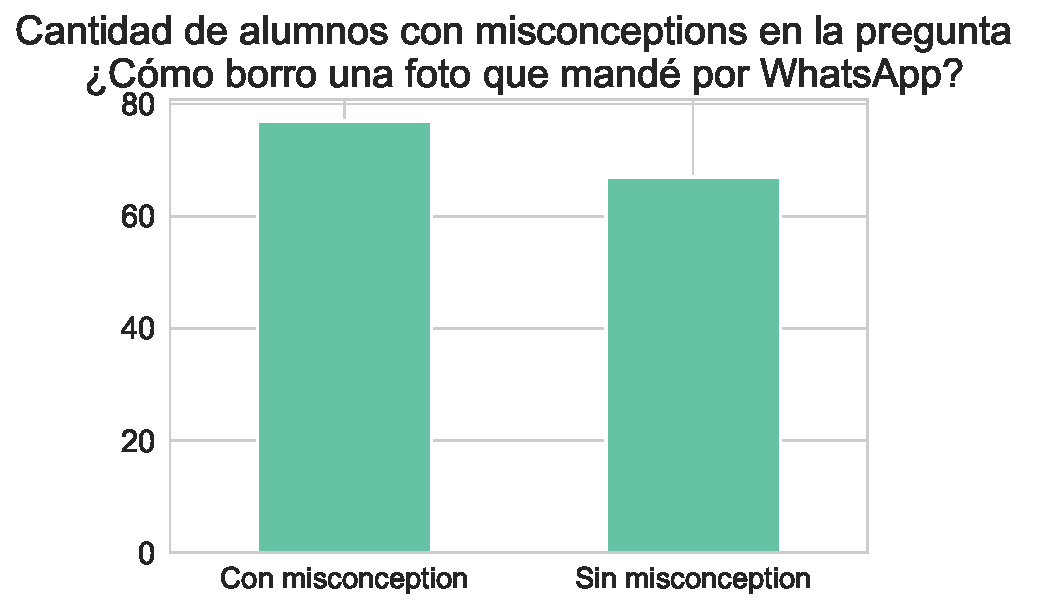
\includegraphics[width=0.5\textwidth]{images_analisis/18.pdf}
    \caption{Cantidad de alumnos con y sin \textit{misconceptions} en la pregunta sobre qué pasa al borrar una foto de un chat.}
    \label{fig:analisis18}
\end{figure}

La opción más elegida fue que \textbf{para dejar de compartir esa foto bastaría con borrarla en el chat de WhatsApp}. Esta respuesta da una idea de que hay una referencia de la foto existente en el servidor de WhatsApp y que al eliminar el mensaje con el archivo en el chat, es suficiente para quitarle el acceso a la otra persona a los datos previamente compartidos.

En contraste, la opción ``No puedo hacer nada, mi amiga ahora también tiene la foto y no tengo manera de sacársela'' intentaba reflejar la idea de que el archivo es compartido mediante una copia, y que una vez que ésta es enviada a la otra persona, se pierde la propiedad sobre la misma y no es posible hacer nada al respecto.
 
\subsection{¿Cómo funciona la red de telefonía móvil?}

El siguiente tema que quisimos explorar fue el funcionamiento de la conectividad móvil. En particular, indagamos sobre cómo viajan los mensajes de WhatsApp cuando no hay WiFi. En la Fig. \ref{fig:analisis19} podemos observar las respuestas obtenidas.

\begin{figure}[h]
    \centering
    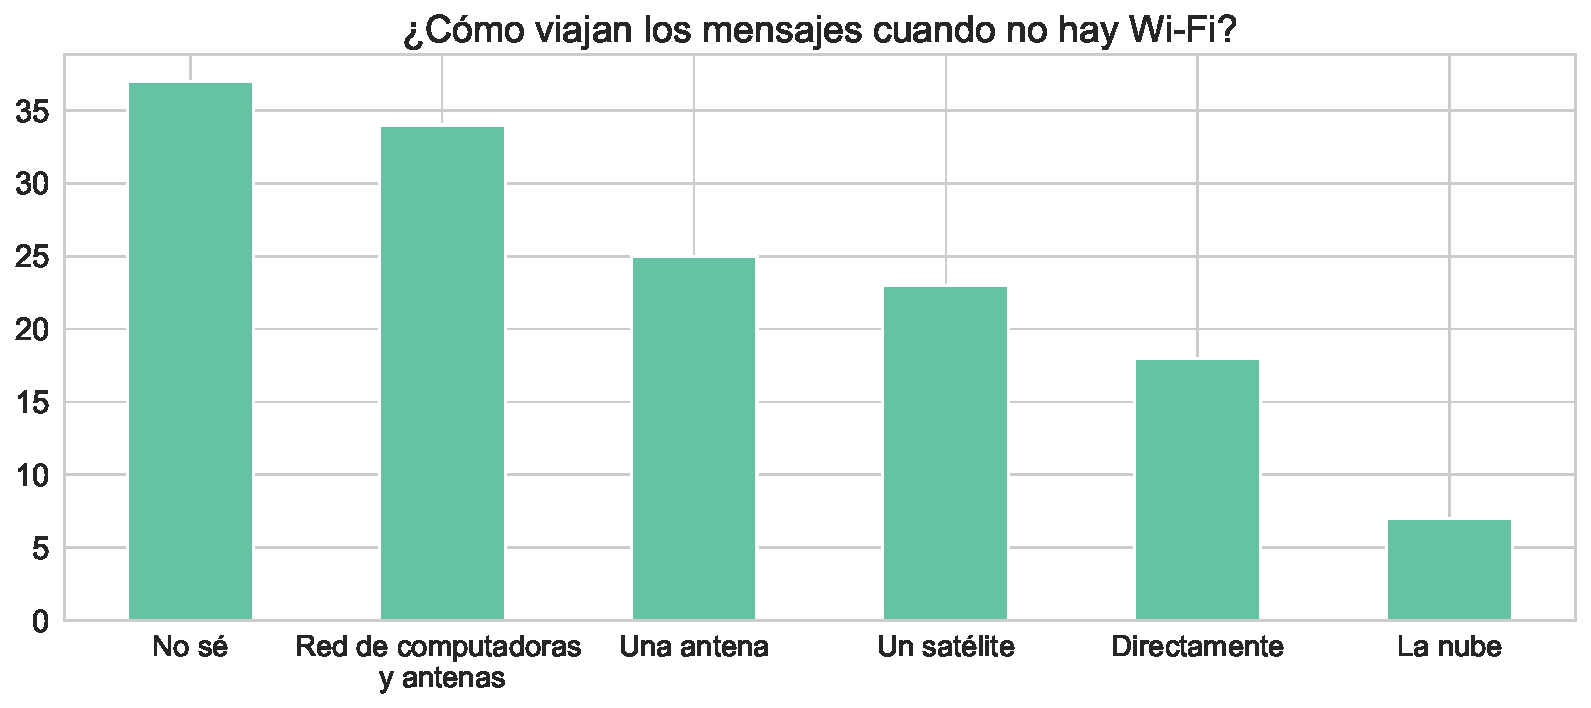
\includegraphics[width=0.9\textwidth]{images_analisis/19.pdf}
    \caption{¿Cómo viajan los mensajes de WhatsApp cuando no hay Wi-Fi?}
    \label{fig:analisis19}
\end{figure}

Es llamativo que en esta pregunta, la opción más elegida fue ``\textit{No sé}''. A pesar de que la gran mayoría de los chicos cuenta con un teléfono celular propio o bien accede a uno que le prestan, vemos que no han llegado a conclusiones respecto a cómo funciona la tecnología de fondo.

De todas formas, una cantidad similar de niños y niñas respondieron a su vez correctamente al elegir la respuesta en la que se proponía que los mensajes viajan a través de una red de antenas y computadoras.
En una proporción semejante aparecen las respuestas en las que se indica que los mensajes viajan a través de una (única) antena, un satélite y ``directamente'' (dando a entender que no existe una infraestructura que intervenga en este proceso).

En la Fig. \ref{fig:analisis20} se muestra un agrupamiento de las respuestas que contienen una \textit{misconception} (en este caso, las que indican que los mensajes viajan a través de la nube, de un satélite, una única antena o directamente) en contraste con la respuesta ``acertada'' (que indicaba que el mensaje viajaba a través de una red de antenas y computadoras) en unión con los que respondieron ``No sé''.

\begin{figure}[h]
    \centering
    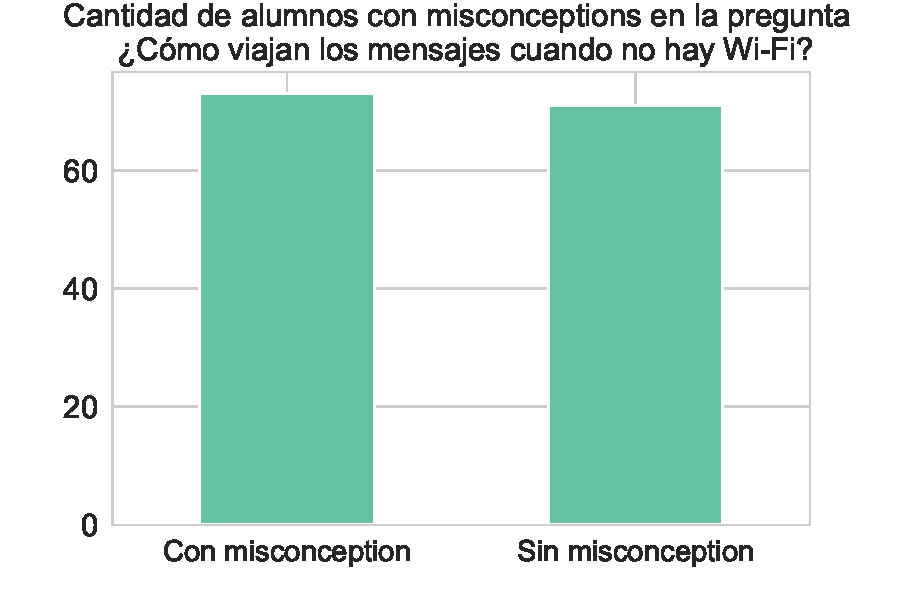
\includegraphics[width=0.6\textwidth]{images_analisis/20.pdf}
    \caption{Cantidad de alumnos con y sin \textit{misconceptions} en la pregunta sobre cómo viajan los mensajes cuando no hay WiFi.}
    \label{fig:analisis20}
\end{figure}

El número de niños y niñas con y sin \textit{misconception} es bastante similar. Veamos ahora si agrupamos las respuestas de otra manera.

\begin{figure}[h]
    \centering
    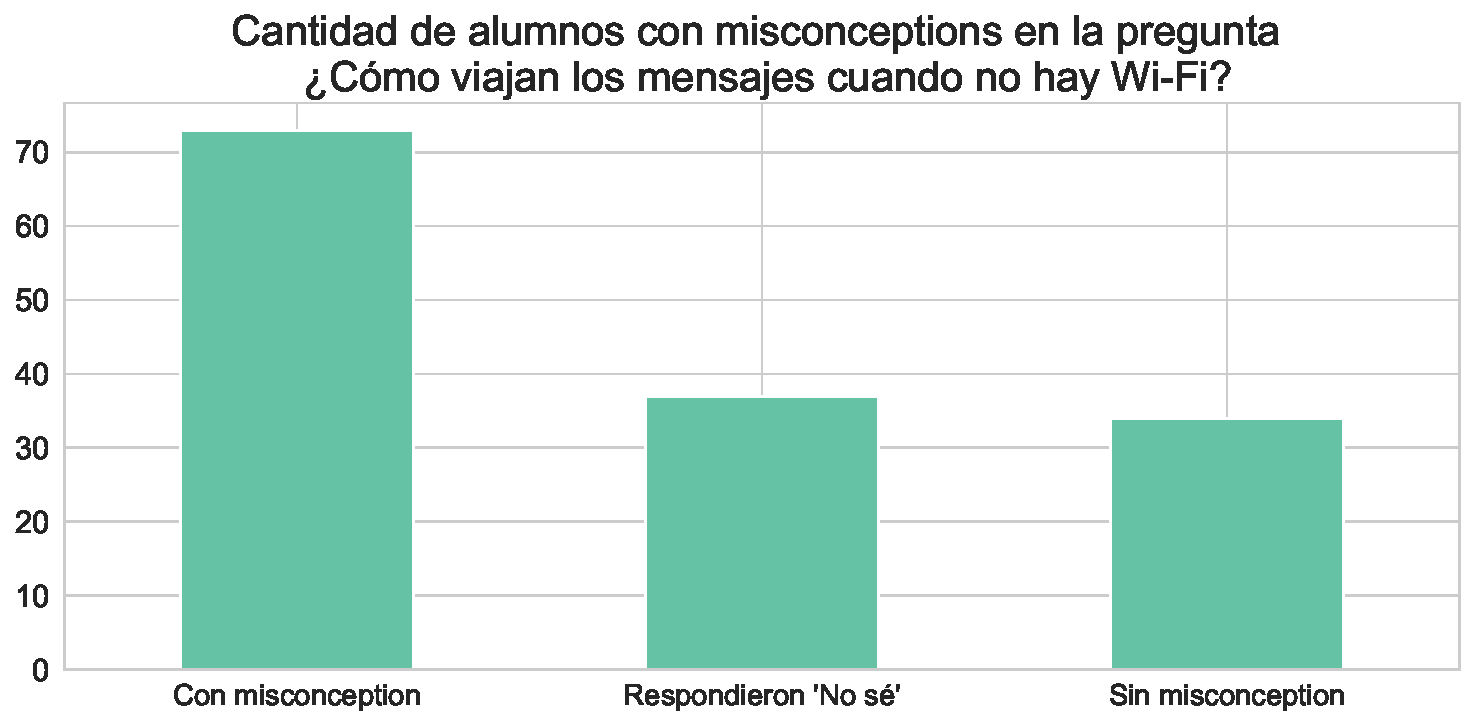
\includegraphics[width=0.7\textwidth]{images_analisis/21.pdf}
    \caption{Alumnos con y sin \textit{misconceptions}, diferenciando a los que respondieron “No sé”.}
    \label{fig:analisis21}
\end{figure}

Si lo analizamos como en la Fig. \ref{fig:analisis21} podemos observar que son más los alumnos que respondieron con \textit{misconception} que los que respondieron correctamente (es decir, sin \textit{misconception}). Más aún: la diferencia es mayor cuando consideramos a los que tienen \textit{misconception} o “no saben”. 

Por último, cabe destacar que la opción de que viajan a través de ``\textit{La nube}'' fue la menos elegida. Y esto es un dato no menor, ya que como habíamos mencionado anteriormente, en la pregunta ``\textit{¿Dónde se almacenan los videos que están en YouTube?}'' la respuesta más elegida fue justamente ``\textit{En la nube}''. Con esta información podemos desentrañar también un poco más cuáles son sus concepciones acerca de ``la nube'': un espacio de almacenamiento ``etéreo'' de datos más que un medio por el cual se envía y recibe información.

\subsection{Gratuidad de las aplicaciones en Internet}


Para conocer las concepciones de los chicos y chicas acerca del por qué de la gratuidad de algunas aplicaciones, les preguntamos ``\textit{¿Por qué hay aplicaciones gratuitas?}'' y, a diferencia de antes, les permitimos a los entrevistados contestar con más de una opción.

\begin{figure}[h]
    \centering
    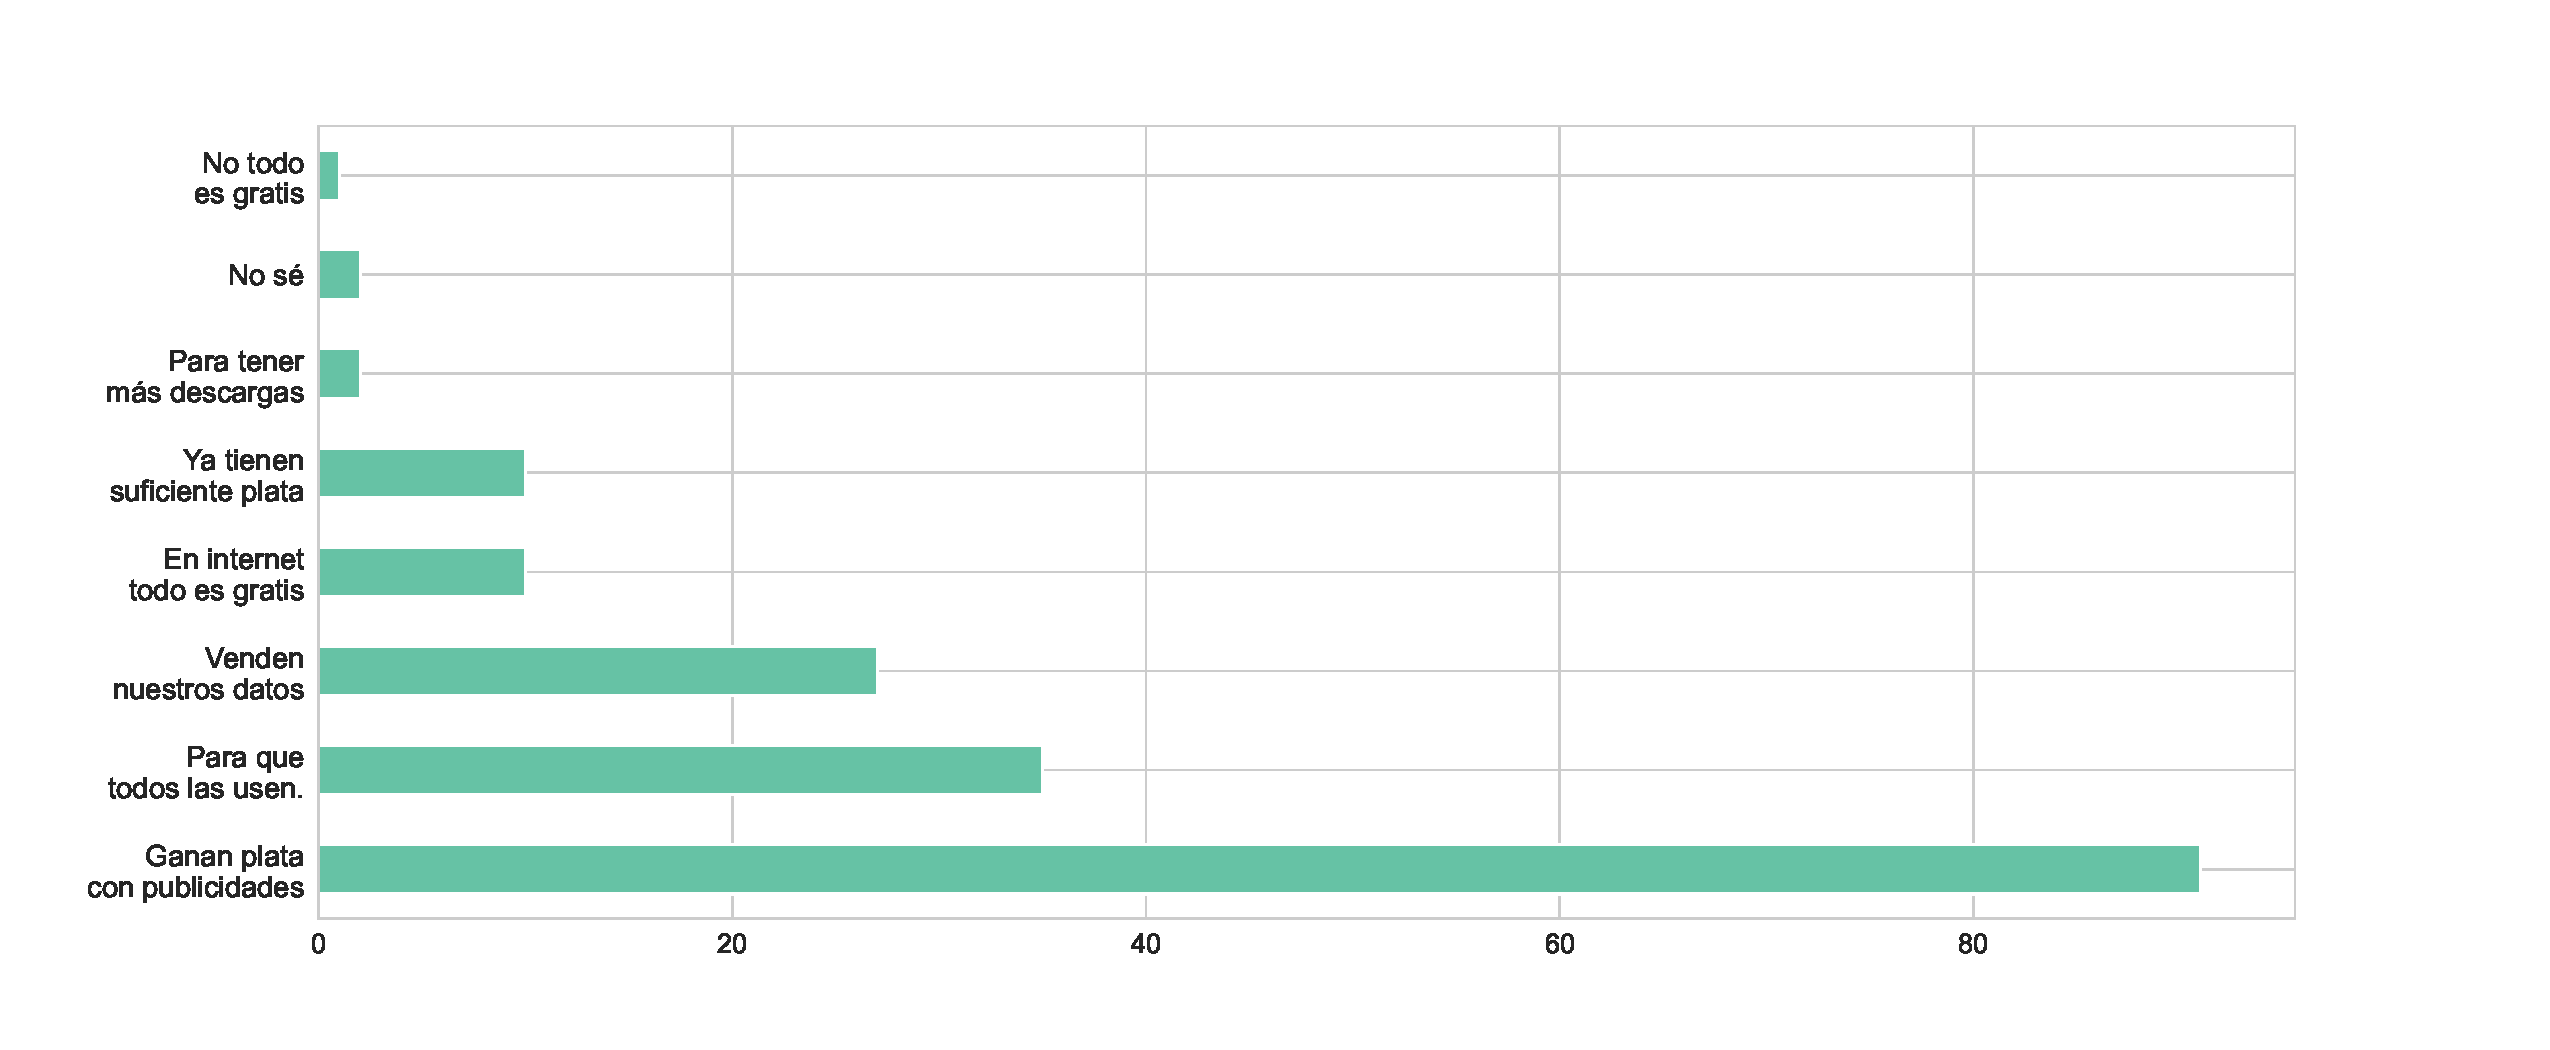
\includegraphics[width=1\textwidth]{images_analisis/22.pdf}
    \caption{Respuestas de la pregunta sobre gratuidad de las aplicaciones, agrupadas por frecuencia de aparición.}
    \label{fig:analisis22}
\end{figure}

En la Fig. \ref{fig:analisis22} mostramos cuáles fueron las opciones más elegidas. La gran mayoría eligió dentro de sus opciones la que propone que la gratuidad de estas es posible gracias al dinero que ganan con las publicidades que nos muestran. Las otras opciones que les habíamos planteado quedaron bastante por detrás en tanto a cantidad de chicos que las eligieron.

Si lo vemos de esta forma, la cantidad de alumnos con y sin \textit{misconception} respecto de este tema es similar, y los que respondieron que no sabían al respecto son realmente muy pocos, como se puede ver en la Fig. \ref{fig:analisis23}.

\begin{figure}[h]
    \centering
    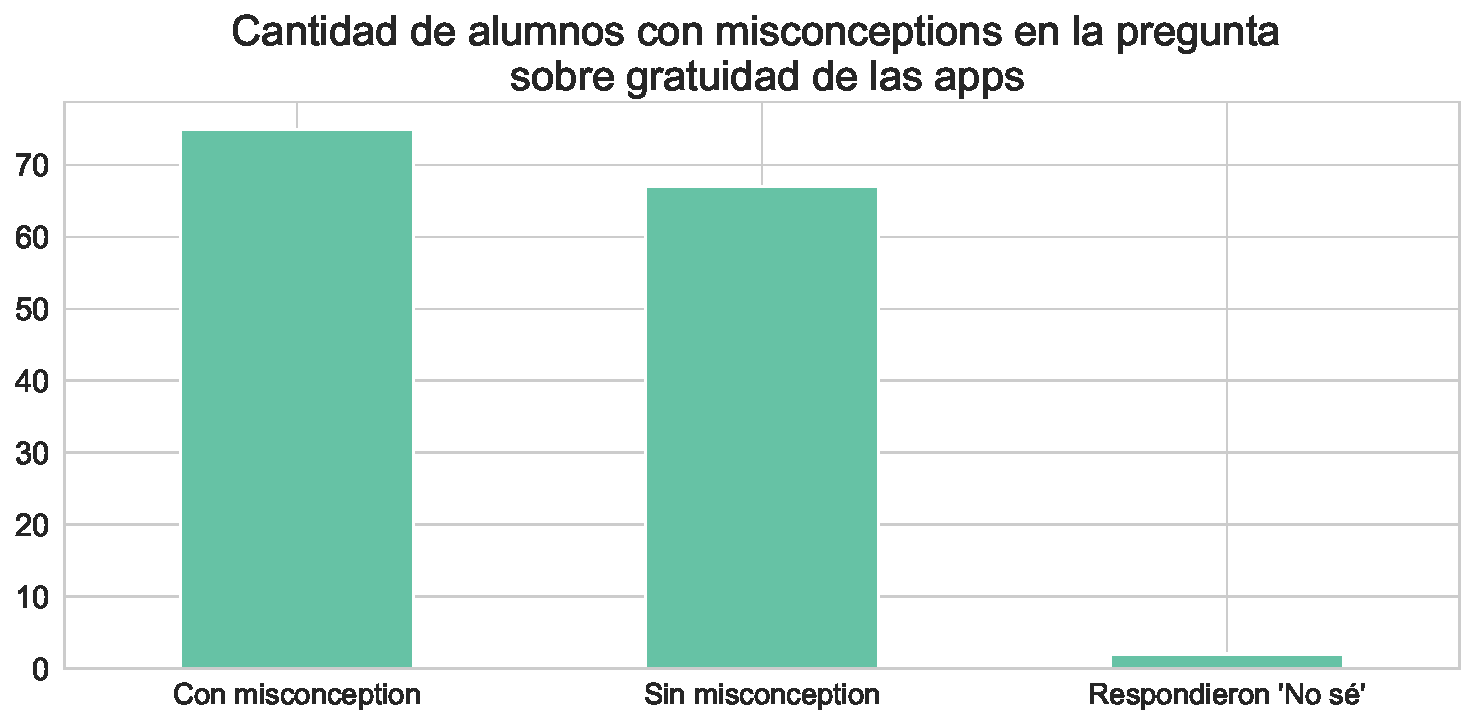
\includegraphics[width=0.75\textwidth]{images_analisis/23.pdf}
    \caption{Cantidad de alumnos con y sin \textit{misconceptions} en la pregunta sobre gratuidad de las aplicaciones en Internet.}
    \label{fig:analisis23}
\end{figure}

\newpage

Sin embargo, dado que en esta pregunta era posible elegir más de una opción, podemos hacer un análisis teniendo en cuenta cuatro grupos: 

\begin{enumerate}
\item Los que respondieron sin \textit{misconception}.
\item Los que respondieron con una \textit{misconception} parcial, es decir, eligieron la respuesta “correcta” junto a otras respuestas con \textit{misconception} (por ejemplo, opinando que las aplicaciones son gratuitas porque ``\textit{ya tienen suficiente dinero y no necesitan más}'' y porque ``\textit{obtienen dinero a través de las publicidades que nos muestran}'').
\item Los que eligieron únicamente respuestas con \textit{misconceptions}.
\item Los que respondieron “No sé”.
\end{enumerate}

\begin{figure}[h]
    \centering
    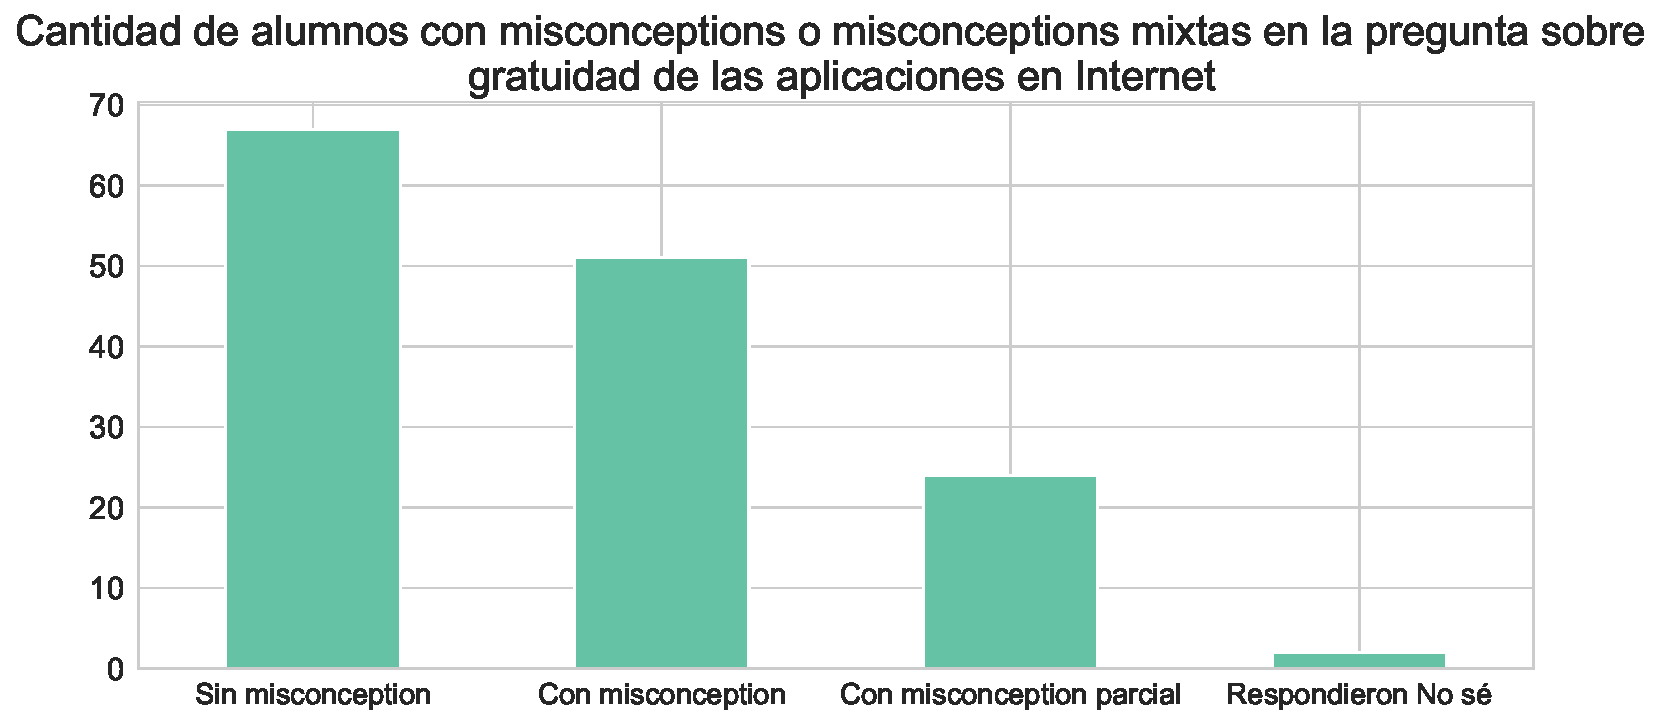
\includegraphics[width=0.75\textwidth]{images_analisis/24.pdf}
    \caption{Cantidad de alumnos con \textit{misconceptions}, sin \textit{misconceptions} y con \textit{misconceptions} parciales en la pregunta sobre gratuidad de las aplicaciones en Internet.}
    \label{fig:analisis24}
\end{figure}


Según esta categorización podemos ver en la Fig. \ref{fig:analisis24} que la cantidad de alumnos sin \textit{misconceptions} es mayor a la cantidad de alumnos con \textit{misconceptions}, o con \textit{misconceptions} parciales.

Es interesante mencionar que en esta pregunta habíamos dejado un casillero libre para completar con otras opciones que se les pudiesen ocurrir y que no estuvieran disponibles. De esta forma, algunos completaron que las aplicaciones son gratis para poder conseguir así ``más descargas en el Play Store''. Según esta respuesta, las aplicaciones ganan más dinero cuantas más descargas consiguen.

La otra respuesta proporcionada por los chicos y chicas fue que ``\textit{No todo es gratis}'' en Internet, dando a entender que también hay aplicaciones que no son gratuitas.

\section{Relación entre las \textit{misconceptions}}

Analicemos ahora si es posible encontrar una relación entre las \textit{misconceptions} que hay en los distintos temas.

Para mayor claridad, nombraremos a las preguntas realizadas para evaluar la presencia o no de \textit{misconceptions} de la siguiente manera:

\begin{table}[h]
\centering
\resizebox{\textwidth}{!}{%
\begin{tabular}{|l|l|}
\hline
¿Dónde se almacenan los videos que están en YouTube? & Pregunta  YouTube     \\ \hline
¿Quién tiene acceso a las fotos que tengo guardadas en mi celular?           & Pregunta Acceso Fotos     \\ \hline
Cuando le mando a una amiga una foto por WhatsApp…   & Pregunta Mandar Fotos \\ \hline
Si quiero hacer que mi amiga no pueda ver más la foto, ¿qué puedo hacer?     & Pregunta Borrar Fotos     \\ \hline
Sofi está en la calle sin WiFi y le quiere mandar un mensaje de WhatsApp.... & Pregunta Mensaje sin WiFi \\ \hline
Muchas de las aplicaciones que conocemos se pueden usar gratuitamente...     & Pregunta Gratuidad Apps   \\ \hline
\end{tabular}%
}
\end{table}

En primer lugar,  revisemos cuántas \textit{misconceptions} tiene cada alumno o alumna en general. En la Fig. \ref{fig:analisis25}, podemos observar que la mayoría de los niños y niñas entrevistados tiene al menos 2 \textit{misconceptions}.

\begin{figure}[h]
    \centering
    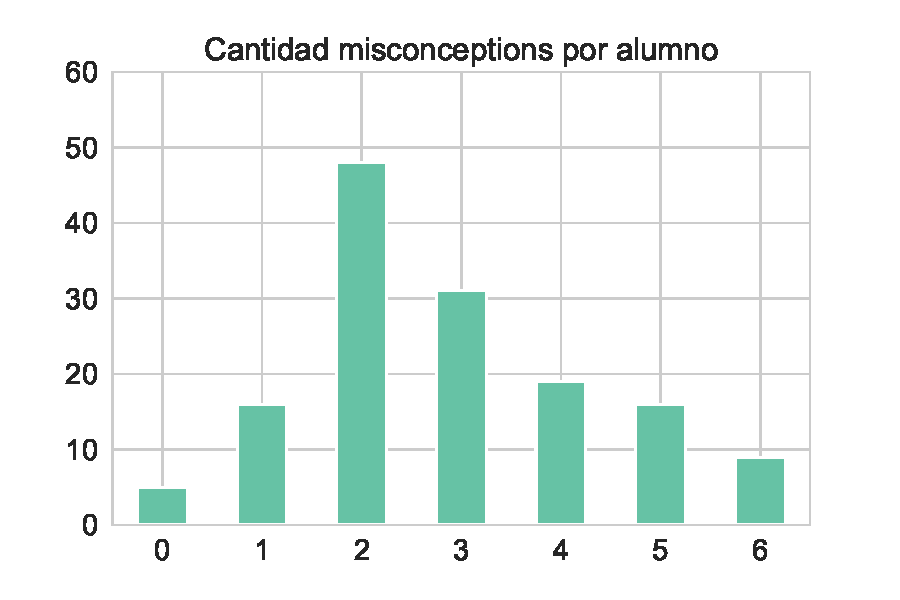
\includegraphics[width=0.55\textwidth]{images_analisis/25.pdf}
    \caption{Cantidad de \textit{misconceptions} por alumno.}
    \label{fig:analisis25}
\end{figure}

Es interesante destacar que tan solo 5 encuestados (es decir, el 3,47\% del total) respondieron a todas las preguntas sin presentar una \textit{misconception}.

Por otro lado, si ordenamos las preguntas en función de cuántos alumnos las respondieron mostrando una \textit{misconception}, podemos ver, como se muestra en la Fig. \ref{fig:analisis26}, que la pregunta ``\textit{¿Dónde se almacenan los videos que están en YouTube?}'' es la que aparece en primer lugar.

\begin{figure}[h]
    \centering
    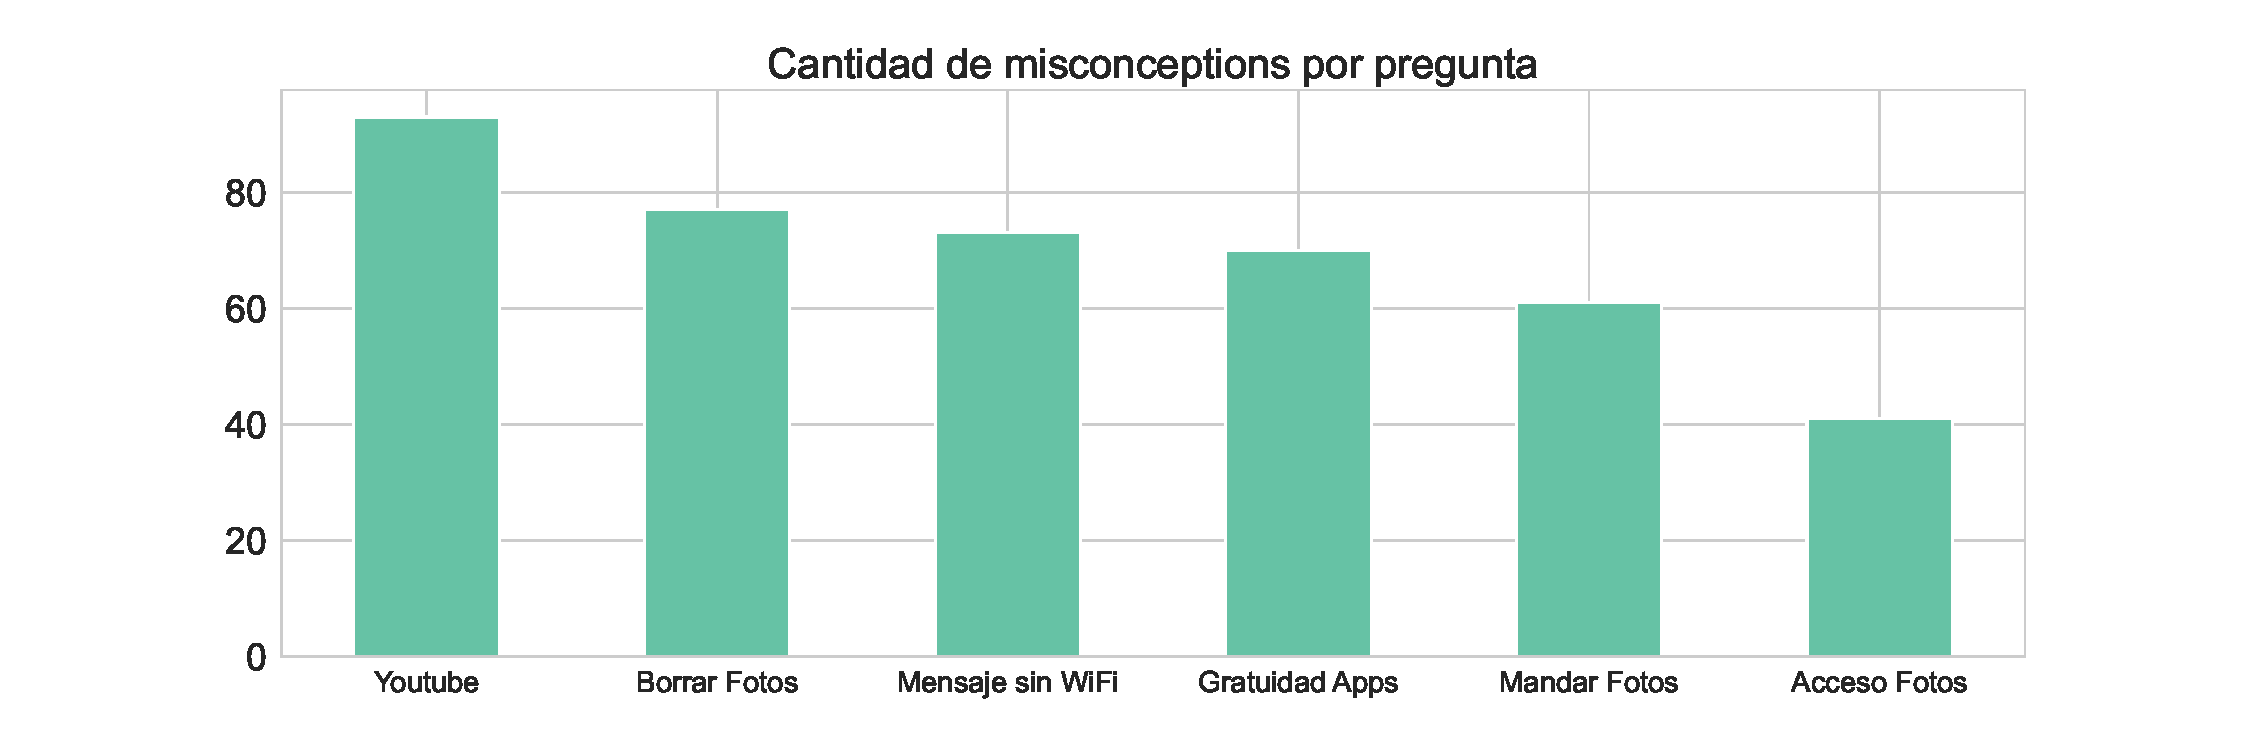
\includegraphics[width=1\textwidth]{images_analisis/26.pdf}
    \caption{\textit{Misconceptions} por pregunta, donde \textit{misconception} parcial no se considera \textit{misconception}.}
    \label{fig:analisis26}  
\end{figure}

\newpage

En segundo lugar, tenemos la pregunta relacionada a si es posible que una persona a la que le compartimos una foto por WhatsApp deje de tener acceso a ésta (``\textit{Si quiero hacer que mi amiga no pueda ver más la foto, ¿qué puedo hacer?}'').

Con casi la misma cantidad de \textit{misconceptions} aparecen la pregunta acerca de cómo viajan los mensajes de WhatsApp cuando no hay WiFi y la pregunta sobre la gratuidad de las aplicaciones en Internet. Sobre esta última cabe destacar que aquí consideramos como \textbf{sin} \textit{misconception} a:

\begin{enumerate}
    \item Los que tenían una \textit{misconception} parcial.
    \item Los que no tenían \textit{misconception}.
    \item Los que respondieron “No sé”.
\end{enumerate}

Si consideramos a los que tenían \textit{misconception} parcial como \textbf{con} \textit{misconception}, entonces como vemos en la Fig. \ref{fig:analisis27}, la distribución cambia y hay más \textit{misconceptions} en esta pregunta que en la de ``\textit{Cómo viajan los mensajes cuando no hay WiFi}''.

\begin{figure}[h]
    \centering
    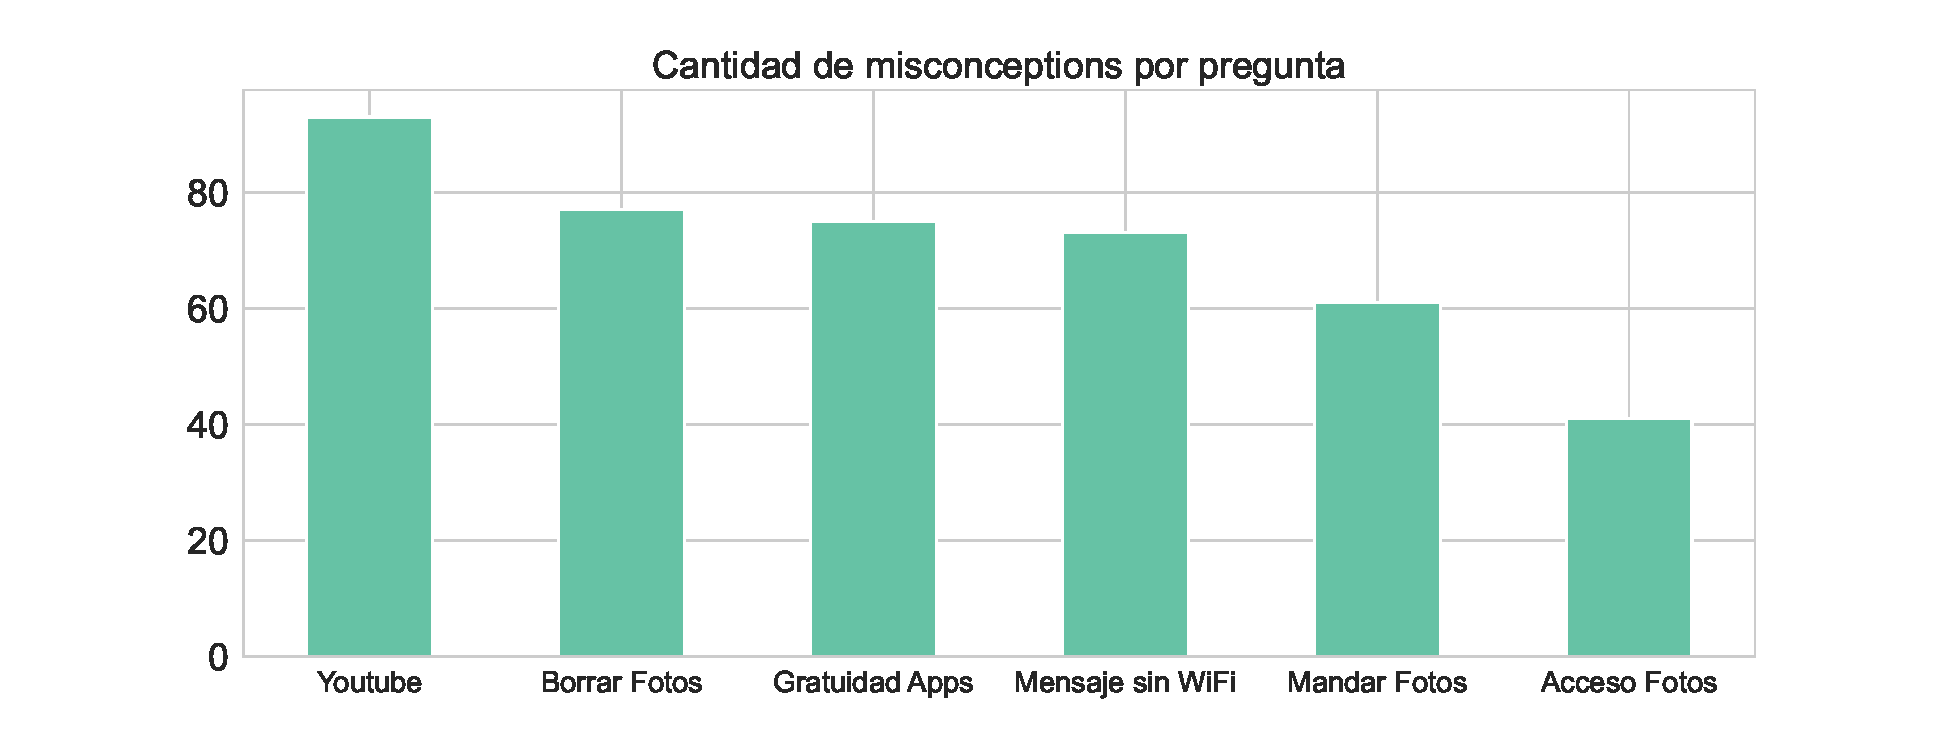
\includegraphics[width=1\textwidth]{images_analisis/27.pdf} 
    \caption{\textit{Misconceptions} por pregunta, donde \textit{misconception} parcial se considera \textit{misconception}.}
    \label{fig:analisis27}
\end{figure}

Por último, analizamos si existe una relación entre las \textit{misconceptions} en las distintas preguntas.

Consideramos para cada pregunta el hecho de si había o no una \textit{misconception} como una variable aleatoria binaria (0 = “no hay \textit{misconception}”, 1 = “hay \textit{misconception}”) y luego medimos la correlación lineal entre ellas usando el método de Pearson. 

Este método devuelve como resultado un valor entre -1 y 1, donde 1 indica una fuerte correlación positiva entre las dos variables (cuando una de las variables es 1 = “hay \textit{misconception}”, la otra también lo es) y -1 muestra una correlación negativa (cuando una de las variables es 1 = “hay \textit{misconception}” la otra es 0 = “no hay \textit{misconception}”). Los valores cercanos a 0 indican que no hay correlación entre las variables.

El \textit{heatmap} que observamos en la Fig. \ref{fig:analisis28} muestra el resultado. 

\begin{figure}[h]
    \centering
    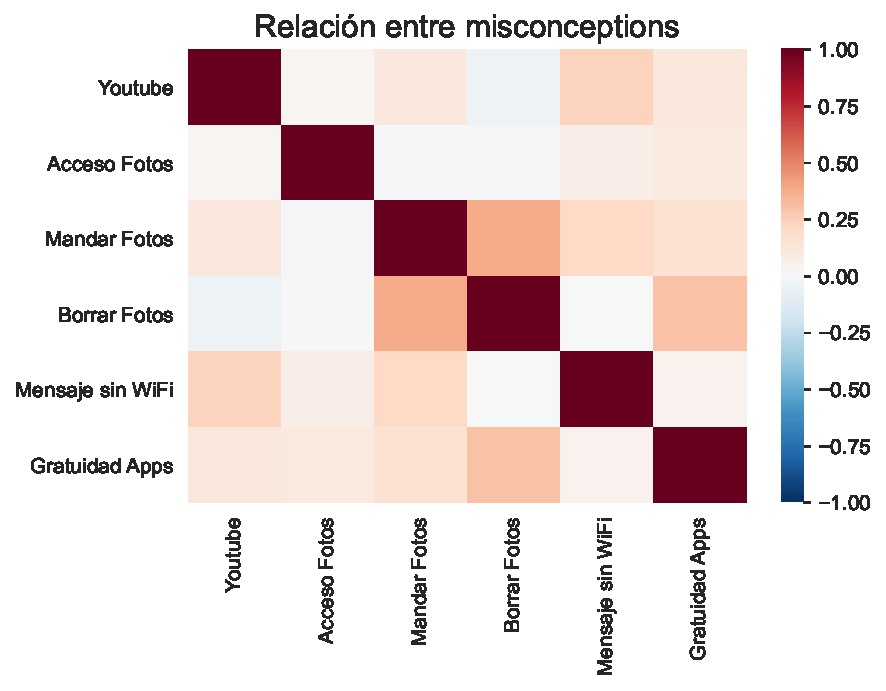
\includegraphics[width=0.7\textwidth]{images_analisis/28.pdf}
    \caption{Relación entre \textit{misconceptions} en las distintas preguntas. }
    \label{fig:analisis28}
\end{figure}

Podemos ver aquí que las preguntas más relacionadas son: ``\textit{Mandar Fotos}'' y ``\textit{Borrar Fotos}''. En ambas buscábamos entender si hay \textit{misconceptions} respecto de si el envío de fotos al utilizar el servicio de mensajería móvil se realiza por copia o referencia, por lo tanto tiene sentido que haya \textit{misconceptions} en ambas preguntas a la vez.

También podemos observar que la pregunta ``\textit{Borrar Fotos}'' se relaciona con ``\textit{Gratuidad Apps}''.

Al mismo tiempo, la pregunta ``\textit{YouTube}'' se encuentra relacionada con ``\textit{Mensajes sin WiFi}''. 

Veamos cómo se relacionan las respuestas de los pares de preguntas, centrándonos en la relación entre las preguntas ``\textit{Mandar Fotos}'' y ``\textit{Borrar Fotos}'' y  ``\textit{YouTube}'' y ``\textit{Mensajes sin WiFi}'' y veamos si este análisis aporta más claridad para entender las relaciones entre las distintas preguntas.

Utilizaremos la siguiente nomenclatura para abreviar las distintas respuestas:

\begin{table}[h]
\centering
\resizebox{\textwidth}{!}{%
\begin{tabular}{|l|l|}
\hline
YouTube - En mi celular                                                               & YouTube - Una compu     \\ \hline
YouTube -  En una computadora                                                         & YouTube - Celular       \\ \hline
YouTube - En la nube                                                                  & YouTube - Nube          \\ \hline
YouTube - En muchas computadoras (tantas que podrían llenar una casa)                 & YouTube - Muchas compus \\ \hline
YouTube - En muchísimas computadoras (tantas que podrían llenar una cancha de fútbol) & YouTube - Muchísimas compus \\ \hline
YouTube - No sé                                                                       & YouTube - No sé         \\ \hline
Mensaje sin WiFI - El mensaje se manda directamente.                                  & Sin WiFi - Directamente \\ \hline
Mensaje sin WiFI - El mensaje se manda a través de la nube.                           & Sin WiFi - Nube         \\ \hline
Mensaje sin WiFI - El mensaje se manda a través de un satélite.                       & Sin WiFi - Satélite     \\ \hline
Mensaje sin WiFI - El mensaje se manda a través de una antena.                        & Sin WiFi - Antena       \\ \hline
Mensaje sin WiFi - El mensaje se manda a través de una red de antenas y computadoras. & Sin WiFi - Red          \\ \hline
Mensaje sin WiFI - No sé                                                              & Sin WiFi - No sé        \\ \hline
Borrar Fotos - Tengo que borrar la foto en el chat.                                   & Borrar - En el chat     \\ \hline
Borrar Fotos - Tengo que borrar la foto en la Galería de fotos de mi celular.         & Borrar - En mi celu     \\ \hline
Borrar Fotos - No puedo hacer nada...                                                 & Borrar - No puedo       \\ \hline
Borrar Fotos - No sé                                                                  & Borrar - No sé          \\ \hline
Mandar Fotos - Le doy permiso para ver la foto que tengo guardada en mi celular.      & Mandar - En mi celu     \\ \hline
Mandar Fotos - Le mando una copia de mi foto                                          & Mandar - copia          \\ \hline
Mandar Fotos - La foto ahora existe en WhatsApp...                                    & Mandar - En WhatsApp    \\ \hline
Mandar Fotos - No sé                                                                  & Mandar - No sé          \\ \hline
\end{tabular}%
}
\end{table}

\newpage

En todos los casos, consideramos como hicimos anteriormente, a cada posible respuesta como una variable aleatoria binaria, donde 0 es “No se eligió dicha respuesta” y 1 es “Se eligió dicha respuesta”. Comprobaremos si hay una correlación lineal entre los pares de preguntas utilizando nuevamente el método de Pearson.

\begin{figure}[h]
    \centering
    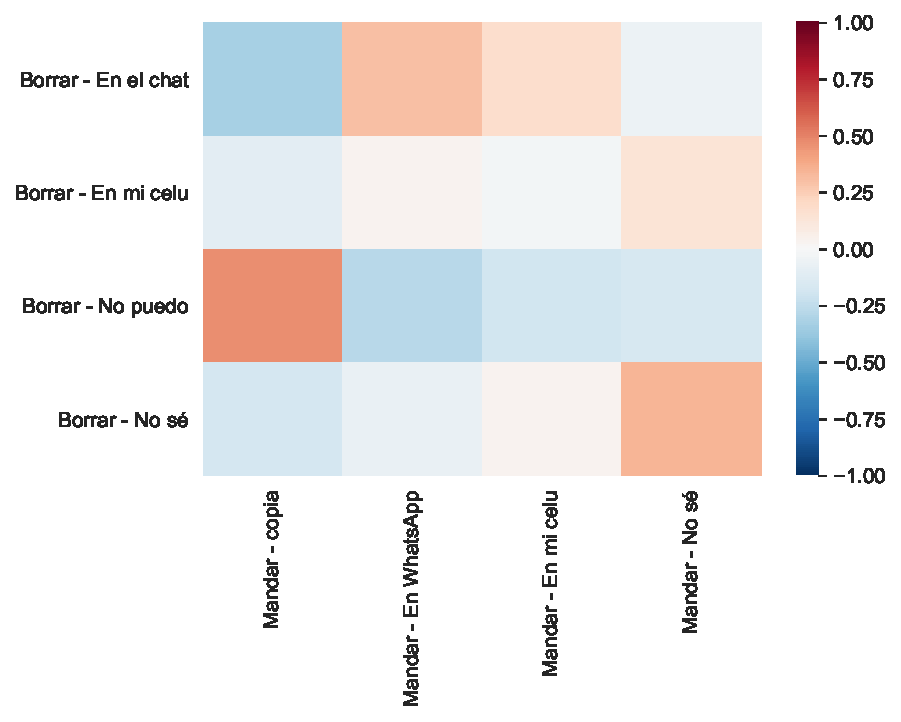
\includegraphics[width=0.7\textwidth]{images_analisis/29.pdf}
    \caption{Relación entre las respuestas a las preguntas “Mandar Fotos” y “Borrar Fotos”.}
    \label{fig:analisis29}
\end{figure}

En la Fig. \ref{fig:analisis29} podemos ver que para las preguntas ``\textit{Mandar Fotos}'' y ``\textit{Borrar Fotos}'' las respuestas que parecieran estar más correlacionadas positivamente (es decir, mayormente los alumnos eligieron estas dos respuestas al responder la encuesta) son:

\begin{itemize}
    \item Borrar- No puedo.
    \item Mandar - copia.
    \item Mandar - No se.
    \item Borrar - No se.
    \item Borrar - En el chat.
    \item Mandar - En WhatsApp.
\end{itemize}

También notamos que hay correlaciones negativas, es decir, mayormente los alumnos no eligieron estas respuestas al mismo tiempo, entre las respuestas:

\begin{itemize}
    \item Borrar - En el chat.
    \item Mandar - copia.
    \item Borrar- No puedo.
    \item Mandar - En WhatsApp.
\end{itemize}

En el caso de las preguntas ``\textit{YouTube}'' y ``\textit{Mensajes sin WiFi}'', es posible observar en la Fig. \ref{fig:analisis30} que las respuestas más correlacionadas positivamente son:

\begin{itemize}
    \item YouTube - Una compu
    \item Sin WiFi - Directamente.
    \item YouTube - Celular.
    \item WiFi - Directamente.
\end{itemize}

\begin{figure}[h]
    \centering
    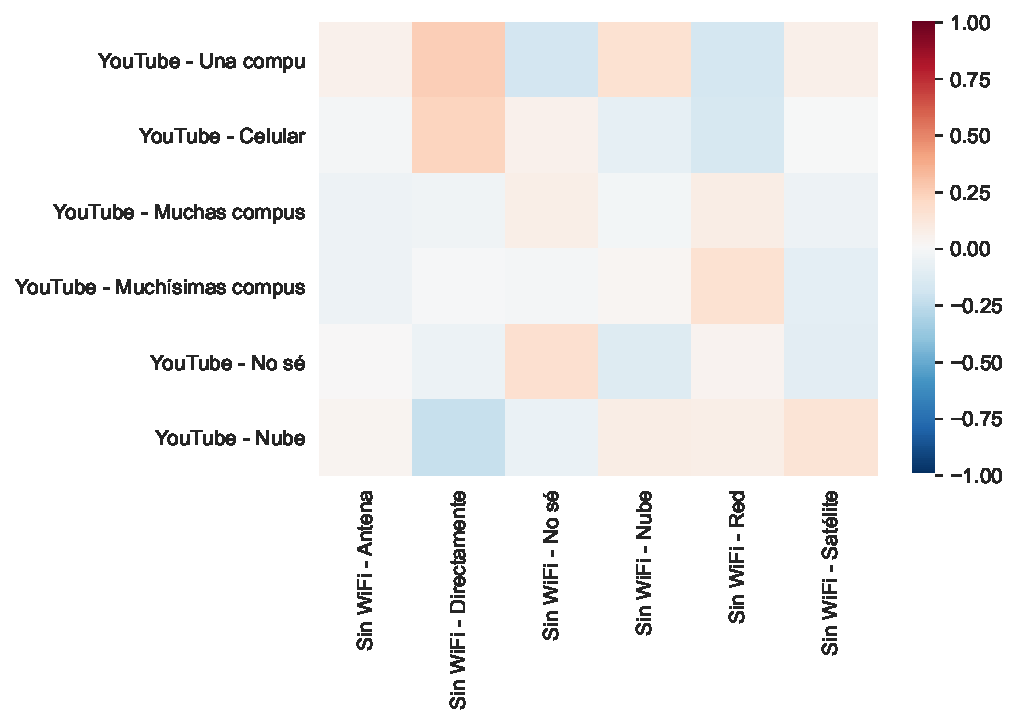
\includegraphics[width=0.65\textwidth]{images_analisis/30.pdf}
    \caption{Relación entre las respuestas a las preguntas ``\textit{YouTube}'' y ``\textit{Mensajes sin WiFi}''.}
    \label{fig:analisis30}
\end{figure}

A su vez, parecería que ``\textit{YouTube - Nube}'' y ``\textit{Sin WiFi - Directamente}'' están correlacionadas negativamente.

Como estamos utilizando variables binarias, decidimos probar para los pares de preguntas que parecían mostrar una mayor correlación con el método de \textit{chi cuadrado}, ya que este es más adecuado para este tipo de variables.

Lo que intentamos es rechazar la hipótesis nula, que en nuestro caso es que dos respuestas dadas son independientes. 

Utilizamos una implementación de \textit{chi cuadrado} de la librería de \textit{Python} \texttt{numpy}, y para ello, en primer lugar realizamos las tablas de correlación de cada par, que muestran cuántos alumnos y alumnas eligieron una, las dos, o ninguna de las respuestas. 

El resultado de la tabla de correlación se puede leer en las tablas expuestas a continuación, que se interpretan de la siguiente manera:

\begin{itemize}
    \item La celda (0,0) en la fila donde se indica “observado'' muestra cuántos alumnos o alumnas no eligieron ninguna de las dos respuestas.
    \item Las celdas (0,1) y (1,0)  en la fila donde se indica “observado'' muestra cuántos alumnos o alumnas eligieron alguna de las dos respuestas.
    \item La celda (1,1), en la fila donde se indica “observado'' muestra cuántos alumnos o alumnas eligieron ambas respuestas.

\end{itemize}

El valor de la fila donde se indica ``esperado'' es el valor que, suponiendo que las respuestas son independientes, deberíamos esperar para esa combinación de respuestas elegidas. Este valor es calculado por el algoritmo \texttt{chi2\_contingency} mencionado anteriormente, pero es interesante presentarlo ya que nos ayudará a interpretar el resultado. Si observo algo que es parecido a lo que esperaba observar (es decir, el ``observado'' es parecido al ``esperado'') entonces no puedo rechazar la hipótesis de que sean variables independientes.

El resultado de realizar el método de chi cuadrado es el p-valor. Un p-valor cercano a 1 no nos permite rechazar la hipótesis nula, es decir, no se puede afirmar que las dos respuestas no sean independientes. Por el contrario, un p-valor cercano a 0 quiere decir que es poco probable observar lo “observado” si las variables son independientes, es decir que podrían estar relacionadas. 

Veamos ahora los resultados para los distintos pares de preguntas comentados previamente.

En la Fig. \ref{fig:analisis32} podemos ver que las respuestas ``\textit{Mandar - copia}'' y ``\textit{Borrar - No puedo}'' parecerían estar altamente correlacionadas, ya que el p-valor obtenido es menor a 0,0001. Este resultado es muy favorable ya que indica que una de las combinaciones de respuestas más frecuentes es de hecho una combinación sin \textit{misconceptions}. Sin embargo, como podemos ver en el campo ``\textit{observado}'', 41 de los chicos (es decir un 28,47\% del total) eligieron estas dos respuestas simultáneamente.

\begin{figure}[h]
    \centering
    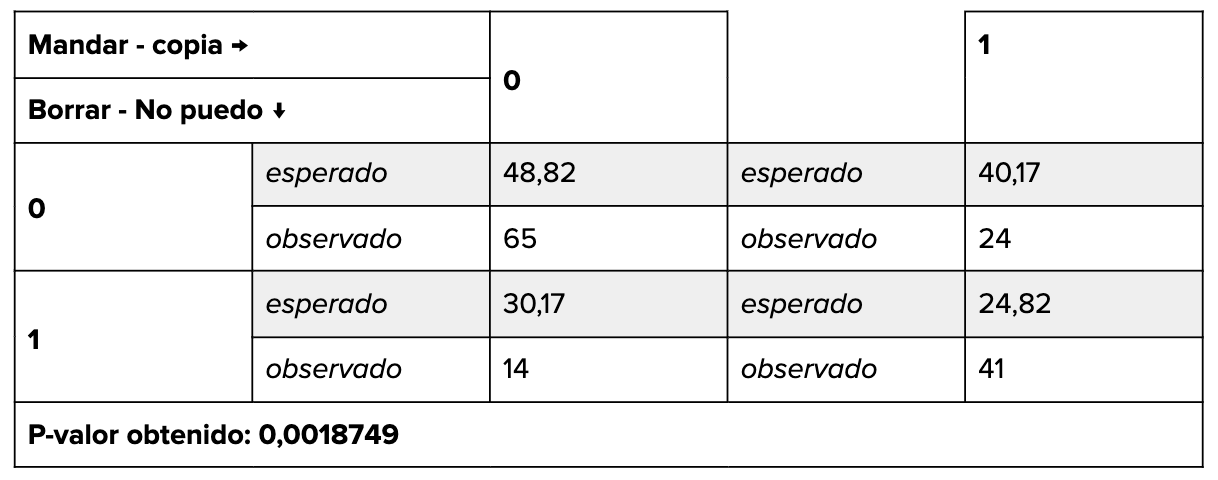
\includegraphics[width=0.65\textwidth]{images_analisis/32.png}
    \caption{Relación entre ``\textit{Mandar - copia}'' y ``\textit{Borrar - No puedo}''}
    \label{fig:analisis32}
\end{figure}

\newpage

Otra observación interesante surge de la Fig. \ref{fig:analisis33}. En esta podemos ver que 38 alumnos (26,38\% del total) eligieron al mismo tiempo las respuestas ``\textit{Mandar - En WhatsApp}'' y ``\textit{Borrar - En el chat}''. El p-valor obtenido al utilizar el método de chi cuadrado corrobora que entre ambas respuestas hay una correlación. Y justamente, estas dos respuestas dan a pensar en la idea de que la información compartida a través de WhatsApp es almacenada de alguna manera ``\textit{remotamente}'' en los servidores del servicio de mensajería, y que no se genera una copia local para la persona a la cual se le compartieron los datos enviados.  

\begin{figure}[h]
    \centering
    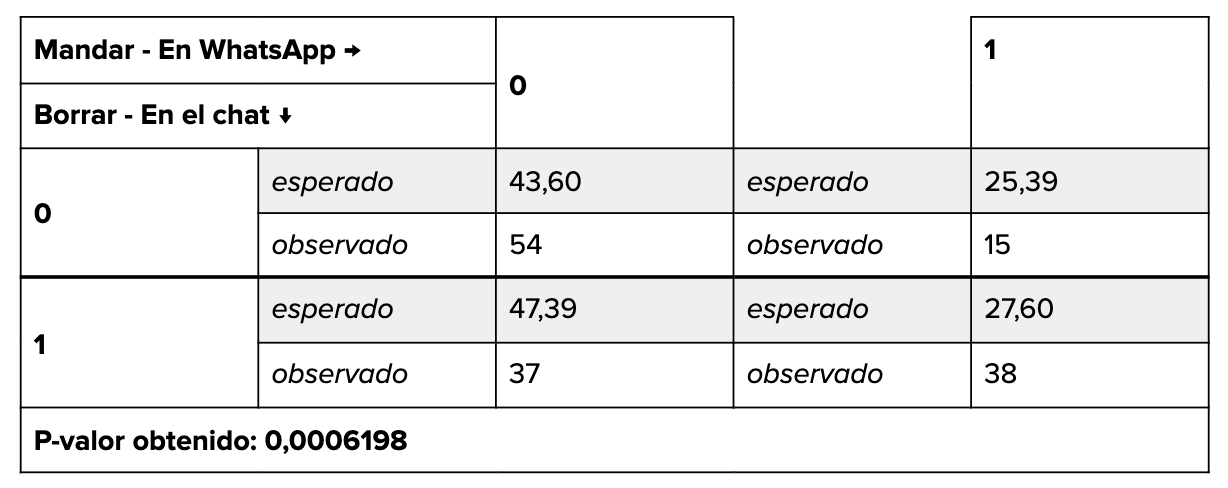
\includegraphics[width=0.65\textwidth]{images_analisis/33.png}
    \caption{Relación entre ``\textit{Mandar - En WhatsApp}'' y ``\textit{Borrar - En el chat}''}
    \label{fig:analisis33}
\end{figure}

En la Fig. \ref{fig:analisis34} observamos que existe correlación entre las respuestas ``\textit{Sin WiFi - Directamente}'' y ``\textit{YouTube - Una compu}''. Esta relación podría interpretarse tal vez como la falta de una noción de la infraestructura subyacente en las tecnologías sobre las que indagamos: por un lado, en la pregunta sobre cómo viajan los mensajes cuando no hay WiFi se responde que los mensajes viajan ``\textit{directamente}'', sin considerar la red sobre la cual se apoya la telefonía móvil. Por otro lado, al responder que los videos en YouTube se almacenan en una única compu queda evidenciado la \textit{misconception} respecto de la cantidad de información de la que hablamos y de la infraestructura necesaria para su almacenamiento.

\begin{figure}[h]
    \centering
    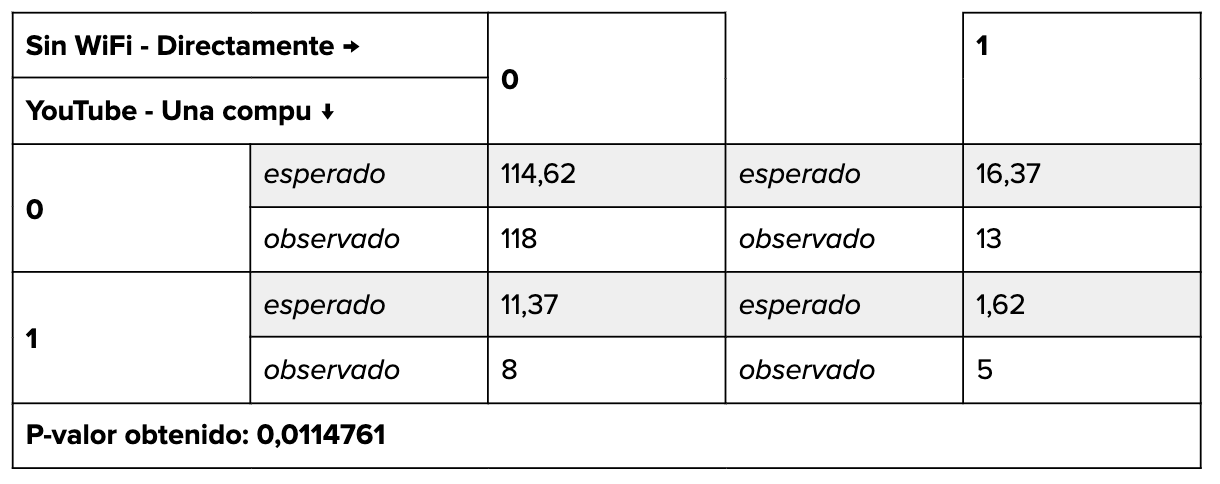
\includegraphics[width=0.65\textwidth]{images_analisis/34.png}
    \caption{Relación entre ``\textit{Sin WiFi - Directamente}'' y ``\textit{YouTube - Una compu}''}
    \label{fig:analisis34}
\end{figure}

\newpage

Una reflexión similar a la anterior podemos hacer con los resultados analizados en la Fig. \ref{fig:analisis35}, en la que vemos que las respuestas ``\textit{Sin WiFi - Directamente}'' y ``\textit{YouTube - Celular}'' se encuentran también relacionadas, pero esta vez, profundizando aún más la \textit{misconception} acerca del volumen de datos que se maneja en YouTube, al responder que los videos se almacenan en ``\textit{un celular}''.

\begin{figure}[h]
    \centering
    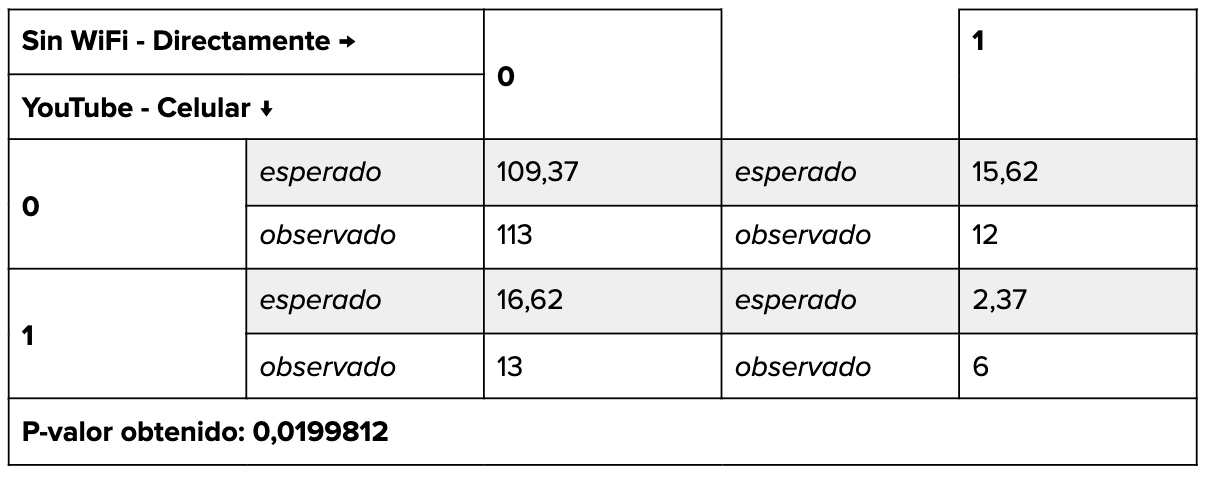
\includegraphics[width=0.65\textwidth]{images_analisis/35.png}
    \caption{Relación entre ``\textit{Sin WiFi - Directamente}'' y ``\textit{YouTube - Celular}''}
    \label{fig:analisis35}
\end{figure}

Adicionalmente, probamos utilizando el método de \textit{clustering aglomerativo}. Con esta técnica se generan \textit{clusters} con los grupos de preguntas más similares, considerando los chicos que respondieron con o sin \textit{misconception}.

El gráfico que se genera se interpreta de la siguiente manera: cada fila representa a un alumno o alumna y cada columna, a una de las preguntas que les propusimos. Cada celda generada se encuentra coloreada en verde oscuro si se respondió con una \textit{misconception} o sin colorear si se respondió sin \textit{misconception}. El algoritmo reordena las filas y columnas de manera de poder visualizar mejor los \textit{clusters} generados, es decir, las preguntas para las cuales se respondió más similarmente. A su vez, produce un dendrograma que muestra los vínculos entre los grupos obtenidos de manera jerárquica. 

En nuestro caso, como se observa en la Fig. \ref{fig:analisis31}, confirmamos que las preguntas más similares son, por un lado, ``\textit{Mandar Fotos}'' y ``\textit{Borrar Fotos}'' y, a su vez, éstas forman un cluster con ``\textit{Gratuidad Apps}''. Por otro lado, la pregunta ``\textit{YouTube}'' y ``\textit{Mensajes sin WiFi}'' forman otro \textit{cluster}.

Es interesante destacar que al utilizar este método visualizamos también cuál es la pregunta que menos se relaciona con las demás. En este caso es ``\textit{Acceso Fotos}''. Un posible motivo por el cuál puede pasar esto es que ésta era una pregunta que, si bien pertenecía al grupo de preguntas sobre el envío de fotos por WhatsApp, su respuesta correcta era bastante accesible al sentido común de los alumnos, y por lo tanto no termina siendo un indicador de si poseen o no \textit{misconceptions} respecto a este tema o a los demás.

\begin{figure}[h]
    \centering
    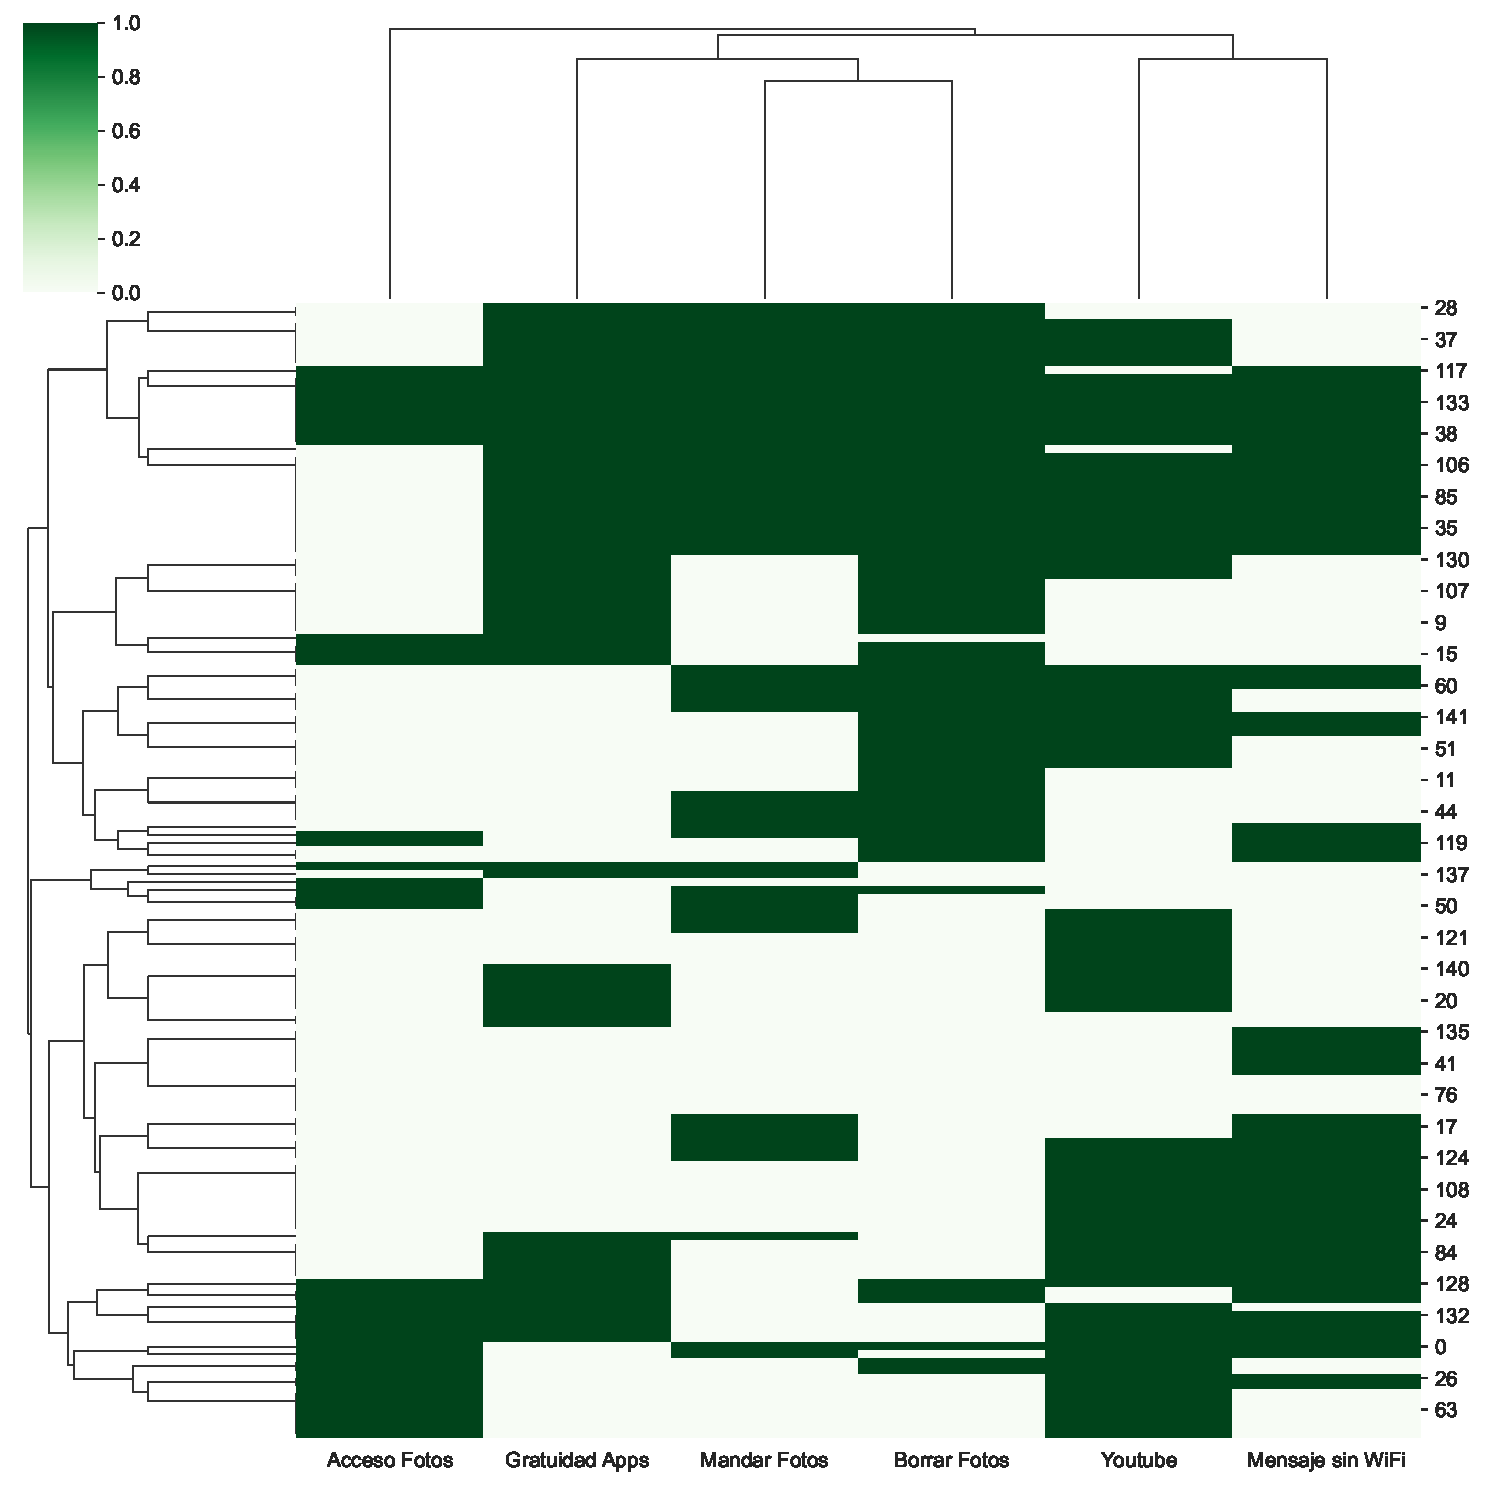
\includegraphics[width=1\textwidth]{images_analisis/31.pdf}
    \caption{\textit{Clustermap} que representa cuáles son las preguntas más relacionadas en función de las respuestas de los alumnos.   }
    \label{fig:analisis31}
\end{figure}
\chapter{Conclusiones y trabajo futuro}
En esta tesis investigamos si niños y niñas de escuelas Argentinas de alrededor de 10 años de edad presentan \textit{misconceptions} en algunos temas de Ciencias de la Computación. En particular, nos centramos en analizar cuáles son sus concepciones respecto a temáticas que les fueran familiares en tanto se encuentran muy presentes en su cotidianidad: dónde se almacenan los videos en YouTube, de qué manera se comparten archivos y cómo viajan los mensajes por WhatsApp y por qué algunas de las aplicaciones que usan diariamente (como TikTok o Instagram, entre otras) son gratis.

Para esto, realizamos una encuesta en la que les planteamos distintas preguntas que les permitieran reflexionar acerca de estos temas. Los chicos y chicas completaron la actividad en un marco de clase online, de manera individual pero con el docente presente. De esta forma, nos aseguramos que sus respuestas fueran lo más “directas” y sin intervención posible, ya que al ser un trabajo en tiempo real, no había posibilidad de hacer preguntas a un adulto o compañero, ni de buscar información en Internet. Una vez que tuvimos sus respuestas, analizamos los datos resultantes para poder entender si había \textit{misconceptions} y cuáles eran estas.

En primer lugar, cabe destacar que gracias a la información poblacional recolectada, pudimos saber que el grupo encuestado estaba ampliamente familiarizado con el conjunto de tecnologías sobre las cuales les preguntamos: son usuarios frecuentes de computadoras y celulares (la mayoría posee computadora en su casa y tiene un celular propio), y utilizan estos dispositivos para variadas actividades, tanto escolares, como recreativas y de socialización. 

A pesar de utilizar YouTube habitualmente, pudimos descubrir que hay \textit{misconceptions} respecto a de qué manera se almacenan los videos en la plataforma: la mayoría de los encuestados piensa que los archivos están guardados en “la nube”. Si bien hubo otras respuestas, pudimos ver que la cantidad de alumnos con alguna \textit{misconception} en este tema fue casi el doble que la de alumnos que respondieron correctamente.

Respecto de la forma en la que se comparten archivos por WhatsApp, observamos que por lo general tienen claro quién tiene acceso a las fotos almacenadas en el propio celular y que al compartir un archivo se envía una copia del mismo. Sin embargo, en el último punto emergió una \textit{misconception}. Cuando les preguntamos si se podía “quitar” el acceso a ese archivo compartido, la mayoría de los encuestados respondió que “bastaba borrar la foto del chat de WhatsApp” para eliminarlo. De esta forma, se hace evidente que la idea de que se ha generado realmente una nueva copia y se ha perdido la propiedad sobre esta no está del todo clara. Este es un punto interesante a trabajar ya que está directamente relacionado con la privacidad de la información compartida y los riesgos que trae la pérdida de la propiedad sobre la misma.

También pudimos ver en nuestros resultados que aún hace falta reforzar los contenidos respecto al funcionamiento de la red de telefonía móvil, ya que la mayoría de los encuestados respondió no saber al respecto, aún siendo que la gran mayoría cuenta con un teléfono celular propio. Un punto llamativo es que, dentro de las opciones que habíamos planteado a la pregunta sobre cómo viajan los mensajes de WhatsApp, habíamos propuesto como una de las opciones “a través de la nube” y esta fue la menos elegida. Esto nos da a entender cuando lo analizamos junto con los resultados de la temática de YouTube comentados anteriormente, que sus concepciones acerca de ``la nube'' tendrían más que ver con un espacio de almacenamiento ``etéreo'' de datos que con un medio por el cual se envía y recibe información. Este punto nos parece interesante para continuar indagando en una siguiente investigación ya que se trata de un término muy presente pero que pareciera tomar distintas interpretaciones, algunas de las cuales podrían tener \textit{misconceptions}.

Sobre la temática referente a la gratuidad de las aplicaciones en Internet pudimos observar que si bien pareciera que muchos de los encuestados tienen concepciones correctas respecto a la pregunta que les planteamos, un gran porcentaje aún conserva una interpretación \textit{naif} o “infantil”. Vale la pena preguntarse aquí si estas \textit{misconceptions} desaparecen y mutan a una visión más adulta sobre cómo funciona el mundo o bien, por el contrario, incluso en los grupos de adultos esta confusión sigue prevaleciendo y falta educar sobre el modelo comercial de las herramientas informáticas de uso cotidiano.

Vale la pena aclarar que las conclusiones mencionadas fueron contrastadas realizando un análisis estadístico que las sustenta.

A futuro y como continuación de este trabajo, sería pertinente ampliar la cantidad de niñas y niños encuestados para poder tener una mejor idea de si los resultados obtenidos son consistentes.

Por otro lado, como mencionamos anteriormente, los alumnos y alumnas encuestados pertenecían a una misma escuela. Consideramos que sería provechoso conseguir la participación de niños y niñas de distintas escuelas de distintos lugares del país para poder analizar los resultados agregando también variables sociales y del contexto educativo de los distintos grupos.

Por último, se podría además variar las edades de los participantes para así entender si hay \textit{misconceptions} que desaparecen o cambian al variar este factor.

\chapter{Anexo: Cuestionario de Investigación}
\label{chap:anexo}
\section{Preguntas poblacionales}
\begin{figure}[H]
    \centering
    
\includegraphics[width=0.8\textwidth]{imagenes_anexo/a.png}
    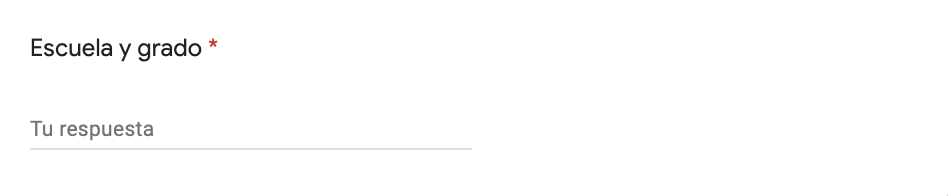
\includegraphics[width=0.8\textwidth]{imagenes_anexo/b.png}
    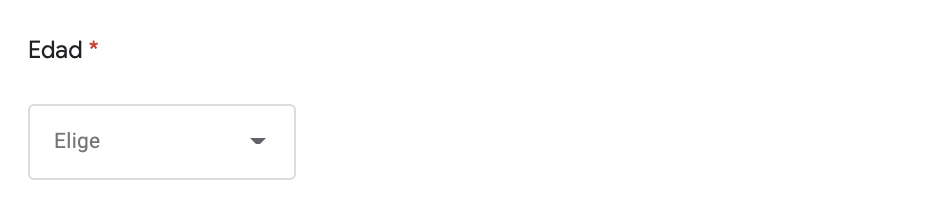
\includegraphics[width=0.8\textwidth]{imagenes_anexo/d.png}
    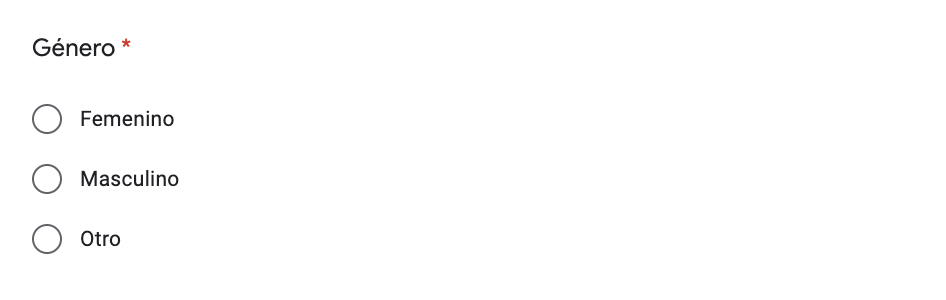
\includegraphics[width=0.8\textwidth]{imagenes_anexo/e.png}
    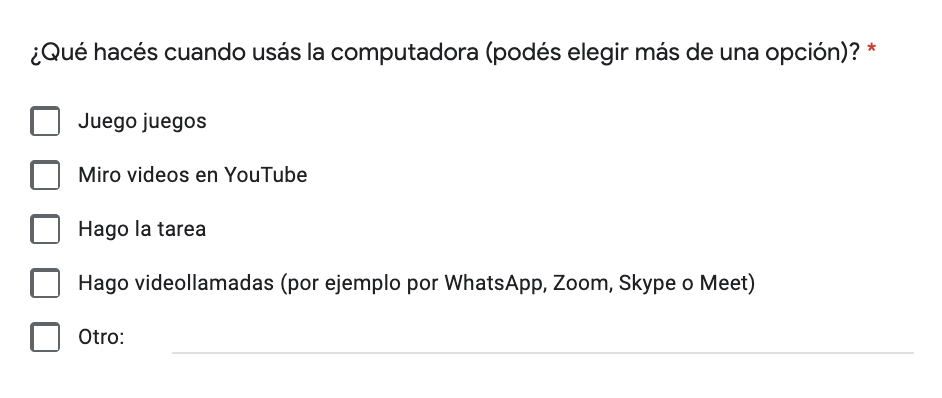
\includegraphics[width=0.8\textwidth]{imagenes_anexo/f.png}
    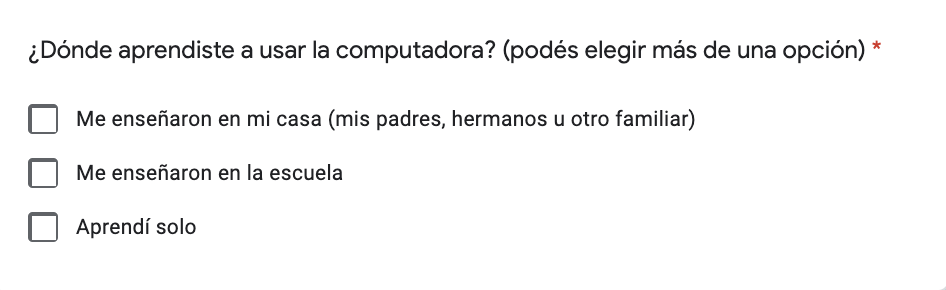
\includegraphics[width=0.8\textwidth]{imagenes_anexo/g.png}
\end{figure}
\begin{figure}[H]
    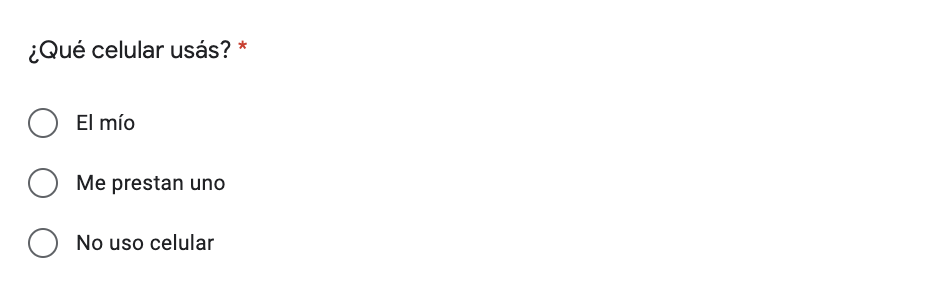
\includegraphics[width=0.8\textwidth]{imagenes_anexo/h.png}
    \includegraphics[width=0.8\textwidth]{imagenes_anexo/i.png}
\end{figure}
\enlargethispage{5\baselineskip}
\section{Preguntas de investigación}
\begin{figure}[H]
    \centering
    \includegraphics[width=0.9\textwidth]{imagenes_anexo/j.png}
    \includegraphics[width=0.9\textwidth]{imagenes_anexo/k.png}
\end{figure}

\begin{figure}[H]
    \includegraphics[width=0.9\textwidth]{imagenes_anexo/l.png}
    \includegraphics[width=0.9\textwidth]{imagenes_anexo/m.png}
    \includegraphics[width=0.9\textwidth]{imagenes_anexo/n.png}
\end{figure}

\begin{figure}[H]    
    \includegraphics[width=0.9\textwidth]{imagenes_anexo/o.png}
\end{figure}

\begin{figure}[H]    
    \includegraphics[width=0.9\textwidth]{imagenes_anexo/p.png}
\end{figure}


\printbibliography %Prints bibliography

%%%% BIBLIOGRAFIA
\backmatter
%\bibliography{tesis}

\end{document}
